\documentclass[11pt,a4paper]{article}

\usepackage[T1]{fontenc}
\usepackage[utf8]{inputenc}
\usepackage{lmodern}
\usepackage{textcomp}
% a true minus sign in text and in math (\textminus alone prints "=" in math mode; set at
% the start of the document, because hyperref redefines it there)
\AtBeginDocument{\DeclareRobustCommand{\textminus}{\ensuremath{-}}}
\usepackage[margin=2.5cm]{geometry}
\usepackage{amsmath,amssymb}
\usepackage{booktabs}
\usepackage{graphicx}
\usepackage{xcolor}
\usepackage[font=small,labelfont=bf]{caption}
\usepackage[authoryear,round]{natbib}
\usepackage{xr-hyper}
\usepackage[colorlinks=true,linkcolor=blue!50!black,citecolor=blue!50!black,urlcolor=blue!50!black]{hyperref}
\usepackage{microtype}
\usepackage{setspace}
% APA 7 citations: the reference list (bib_paper.tex) is generated by analysis/apa_refs.py;
% two authors are joined by "and" in narrative and by "&" in parenthetical citations
\newif\ifapaparen
\DeclareRobustCommand{\apaand}{\ifapaparen\&\else and\fi}
\NewCommandCopy{\natcitep}{\citep}
\RenewDocumentCommand{\citep}{o o m}{{\apaparentrue%
  \IfNoValueTF{#1}{\natcitep{#3}}{\IfNoValueTF{#2}{\natcitep[#1]{#3}}{\natcitep[#1][#2]{#3}}}}}
\setstretch{1.08}
\emergencystretch=2em

% Every quoted result is a macro generated from the study's JSON outputs
% by analysis/make_tables.py; see the Code availability statement.
% Status labels: [pre-specified] and [exploratory] are stated in the text
% where each analysis is introduced (Section 4 lists them).
\newcommand{\sh}{\ensuremath{\sharp}}
\newcommand{\flip}[1]{\textbf{#1}}
% AUTO-GENERATED by analysis/make_tables.py -- do not edit by hand.
\newcommand{\ratingTT}{1.953}
\newcommand{\ratingMsix}{2.477}
\newcommand{\nBelowTT}{4}
\newcommand{\gapClarCFourS}{\textminus{}3.4}
\newcommand{\gapClarCFourSmin}{+6.8}
\newcommand{\gapClarCFourV}{+39.8}
\newcommand{\gapClarCFourHK}{\textminus{}46.6}
\newcommand{\gapBassoonHK}{+55.0}
\newcommand{\gapHornV}{+198.1}
\newcommand{\shareInstrAll}{26}
\newcommand{\shareModelAll}{16}
\newcommand{\shareInterAll}{58}
\newcommand{\shareInstrLRAll}{34}
\newcommand{\shareModelLRAll}{18}
\newcommand{\shareInterLRAll}{48}
\newcommand{\signModelAll}{11/48}
\newcommand{\signModelPctAll}{23}
\newcommand{\signInstrAll}{45/112}
\newcommand{\signInstrPctAll}{40}
\newcommand{\medRangeModelsAll}{34.6}
\newcommand{\medRangeInstrAll}{97.7}
\newcommand{\shareInstrNoV}{55}
\newcommand{\shareModelNoV}{8}
\newcommand{\shareInterNoV}{36}
\newcommand{\shareInstrLRNoV}{56}
\newcommand{\shareModelLRNoV}{11}
\newcommand{\shareInterLRNoV}{33}
\newcommand{\signModelNoV}{6/24}
\newcommand{\signModelPctNoV}{25}
\newcommand{\signInstrNoV}{38/84}
\newcommand{\signInstrPctNoV}{45}
\newcommand{\medRangeModelsNoV}{20.0}
\newcommand{\medRangeInstrNoV}{93.8}
\newcommand{\shareInstrRegAll}{26}
\newcommand{\shareModelRegAll}{36}
\newcommand{\shareInterRegAll}{38}
\newcommand{\shareInstrLRRegAll}{25}
\newcommand{\shareModelLRRegAll}{44}
\newcommand{\shareInterLRRegAll}{31}
\newcommand{\signModelRegAll}{20/54}
\newcommand{\signModelPctRegAll}{37}
\newcommand{\signInstrRegAll}{44/144}
\newcommand{\signInstrPctRegAll}{31}
\newcommand{\medRangeModelsRegAll}{53.8}
\newcommand{\medRangeInstrRegAll}{70.8}
\newcommand{\shareInstrRegNoV}{43}
\newcommand{\shareModelRegNoV}{30}
\newcommand{\shareInterRegNoV}{27}
\newcommand{\shareInstrLRRegNoV}{39}
\newcommand{\shareModelLRRegNoV}{34}
\newcommand{\shareInterLRRegNoV}{28}
\newcommand{\signModelRegNoV}{10/27}
\newcommand{\signModelPctRegNoV}{37}
\newcommand{\signInstrRegNoV}{44/108}
\newcommand{\signInstrPctRegNoV}{41}
\newcommand{\medRangeModelsRegNoV}{18.0}
\newcommand{\medRangeInstrRegNoV}{58.3}
\newcommand{\rangeClarKernels}{86.4}
\newcommand{\rangeHKInstr}{101.6}
\newcommand{\sensKernelMed}{18.0}
\newcommand{\sensKernelMax}{76.0}
\newcommand{\sensRecordingMed}{6.0}
\newcommand{\sensRecordingMax}{31.5}
\newcommand{\sensExtractionMed}{0.4}
\newcommand{\sensExtractionMax}{2.8}
\newcommand{\sensCodecMed}{0.3}
\newcommand{\sensCodecMax}{1.2}
\newcommand{\sensIdealMed}{8.8}
\newcommand{\sensIdealMax}{19.1}
\newcommand{\sensABWideMed}{39.4}
\newcommand{\sensABWideMax}{129.8}
\newcommand{\sensABNarrowMed}{13.9}
\newcommand{\sensABNarrowMax}{41.1}
\newcommand{\sensInstrMed}{93.8}
\newcommand{\sensInstrMax}{101.6}
\newcommand{\sensVassExtractMax}{168.3}
\newcommand{\sensVassExtractMed}{9.3}
\newcommand{\codecWorstVass}{3.6}
\newcommand{\codecWorstStable}{0.9}
\newcommand{\extrVassWorst}{134.1}
\newcommand{\extrHKWorst}{2.8}
\newcommand{\hornVassLoose}{+64.0}
\newcommand{\idealHKFlat}{\textminus{}3.2}
\newcommand{\idealHKBase}{+4.6}
\newcommand{\iowaHKDThree}{\textminus{}22.1}
\newcommand{\philHKDThree}{\textminus{}30.8}
\newcommand{\diffHKDThree}{8.7}
\newcommand{\eoIowaDThree}{0.405}
\newcommand{\eoPhilDThree}{0.487}
\newcommand{\iowaHKCFour}{\textminus{}43.0}
\newcommand{\philHKCFour}{\textminus{}46.6}
\newcommand{\diffHKCFour}{3.6}
\newcommand{\eoIowaCFour}{0.194}
\newcommand{\eoPhilCFour}{0.178}
\newcommand{\iowaHKCFive}{\textminus{}11.7}
\newcommand{\philHKCFive}{\textminus{}43.2}
\newcommand{\diffHKCFive}{31.5}
\newcommand{\eoIowaCFive}{0.347}
\newcommand{\eoPhilCFive}{0.089}
\newcommand{\sethCFiveIowa}{\textminus{}7.4}
\newcommand{\sethCFivePhil}{+15.3}
\newcommand{\mechHKpairShare}{70}
\newcommand{\mechHKpairBeat}{62}
\newcommand{\mechHKpairFlo}{1304}
\newcommand{\mechHKpairFhi}{1242}
\newcommand{\mechSethFundShare}{36}
\newcommand{\mechSethFundBeat}{108}
\newcommand{\mechFundCBW}{1.49}
\newcommand{\mechFundERB}{1.84}
\newcommand{\mechHKTTovMsix}{0.53}
\newcommand{\mechCelloFundShare}{73}
\newcommand{\abStableWide}{7}
\newcommand{\abStableNarrow}{11}
\newcommand{\abNSpectra}{17}
\newcommand{\abUnstableNarrow}{cello C3, cello C4, French horn C4, oboe C4, oboe C5, piano C4}
\newcommand{\cutCelloCFour}{+3.7}
\newcommand{\gapCelloCFourHK}{\textminus{}1.7}
\newcommand{\gapHornHK}{\textminus{}0.6}
\newcommand{\clarHKExtrMax}{1.5}
\newcommand{\clarCutMaxRange}{1.8}
\newcommand{\abUnstableMaxAbs}{11.7}
\newcommand{\abClarPositiveCells}{Philharmonia D3: $a=0.35, b=1$; Iowa D3: $a=0.35, b=1$, $a=0.35, b=1.5$}
\newcommand{\mechFundMean}{315}
\newcommand{\mechFundGpct}{0.17}
\newcommand{\erbSignChanges}{cello C4, oboe C4}
\newcommand{\erbNSignChanges}{2}
\newcommand{\pianoB}{3.17}
\newcommand{\pianoBse}{6.3}
\newcommand{\pianoResid}{0.005}
\newcommand{\pianoTopRatio}{15.52}
\newcommand{\vassExpSignChanges}{3}
\newcommand{\vassExpNSpectra}{17}
\newcommand{\abGridA}{0.15, 0.2, 0.25, 0.3, 0.35}
\newcommand{\abGridB}{1.0, 1.5, 2.0, 2.5, 3.0}
\newcommand{\hkGapRaw}{0.233}
\newcommand{\hkGapZ}{0.120}
\newcommand{\hkGapMean}{0.085}
\newcommand{\dRBRawI}{0.049}
\newcommand{\pRBRawI}{$p<.001$}
\newcommand{\dRBRawH}{0.010}
\newcommand{\pRBRawH}{$p=.004$}
\newcommand{\dRBRawF}{0.147}
\newcommand{\pRBRawF}{$p<.001$}
\newcommand{\RfullBRaw}{0.674}
\newcommand{\dRBSizeI}{0.075}
\newcommand{\pRBSizeI}{$p<.001$}
\newcommand{\dRBSizeH}{0.037}
\newcommand{\pRBSizeH}{$p<.001$}
\newcommand{\dRBSizeF}{0.080}
\newcommand{\pRBSizeF}{$p<.001$}
\newcommand{\RfullBSize}{0.738}
\newcommand{\dRBRegI}{0.085}
\newcommand{\pRBRegI}{$p<.001$}
\newcommand{\dRBRegH}{0.042}
\newcommand{\pRBRegH}{$p<.001$}
\newcommand{\dRBRegF}{0.058}
\newcommand{\pRBRegF}{$p<.001$}
\newcommand{\RfullBReg}{0.749}
\newcommand{\dRBTrI}{0.074}
\newcommand{\pRBTrI}{$p<.001$}
\newcommand{\dRBTrH}{0.043}
\newcommand{\pRBTrH}{$p<.001$}
\newcommand{\dRBTrF}{0.082}
\newcommand{\pRBTrF}{$p<.001$}
\newcommand{\RfullBTr}{0.737}
\newcommand{\rHKBRaw}{0.713}
\newcommand{\rankHKBRaw}{4}
\newcommand{\rHuronBRaw}{0.685}
\newcommand{\rankHuronBRaw}{5}
\newcommand{\rSethBRaw}{0.393}
\newcommand{\rankSethBRaw}{14}
\newcommand{\rVassBRaw}{0.389}
\newcommand{\rankVassBRaw}{15}
\newcommand{\rCorpusBRaw}{0.722}
\newcommand{\rankCorpusBRaw}{3}
\newcommand{\rStolzBRaw}{0.740}
\newcommand{\rankStolzBRaw}{2}
\newcommand{\rCompositeBRaw}{0.801}
\newcommand{\rankCompositeBRaw}{1}
\newcommand{\rHKBSize}{0.761}
\newcommand{\rankHKBSize}{3}
\newcommand{\rHuronBSize}{0.692}
\newcommand{\rankHuronBSize}{5}
\newcommand{\rSethBSize}{0.521}
\newcommand{\rankSethBSize}{12}
\newcommand{\rVassBSize}{0.455}
\newcommand{\rankVassBSize}{14}
\newcommand{\rCorpusBSize}{0.719}
\newcommand{\rankCorpusBSize}{4}
\newcommand{\rStolzBSize}{0.794}
\newcommand{\rankStolzBSize}{2}
\newcommand{\rCompositeBSize}{0.856}
\newcommand{\rankCompositeBSize}{1}
\newcommand{\rHKBReg}{0.771}
\newcommand{\rankHKBReg}{3}
\newcommand{\rHuronBReg}{0.706}
\newcommand{\rankHuronBReg}{5}
\newcommand{\rSethBReg}{0.540}
\newcommand{\rankSethBReg}{11}
\newcommand{\rVassBReg}{0.477}
\newcommand{\rankVassBReg}{14}
\newcommand{\rCorpusBReg}{0.722}
\newcommand{\rankCorpusBReg}{4}
\newcommand{\rStolzBReg}{0.796}
\newcommand{\rankStolzBReg}{2}
\newcommand{\rCompositeBReg}{0.857}
\newcommand{\rankCompositeBReg}{1}
\newcommand{\rHKBTr}{0.751}
\newcommand{\rankHKBTr}{3}
\newcommand{\rHuronBTr}{0.692}
\newcommand{\rankHuronBTr}{5}
\newcommand{\rSethBTr}{0.540}
\newcommand{\rankSethBTr}{12}
\newcommand{\rVassBTr}{0.453}
\newcommand{\rankVassBTr}{14}
\newcommand{\rCorpusBTr}{0.719}
\newcommand{\rankCorpusBTr}{4}
\newcommand{\rStolzBTr}{0.794}
\newcommand{\rankStolzBTr}{2}
\newcommand{\rCompositeBTr}{0.855}
\newcommand{\rankCompositeBTr}{1}
\newcommand{\dRJRawI}{0.005}
\newcommand{\pRJRawI}{$p=.344$}
\newcommand{\dRJRawH}{0.042}
\newcommand{\pRJRawH}{$p=.009$}
\newcommand{\dRJRawF}{0.141}
\newcommand{\pRJRawF}{$p<.001$}
\newcommand{\RfullJRaw}{0.414}
\newcommand{\dRJSizeI}{0.033}
\newcommand{\pRJSizeI}{$p=.013$}
\newcommand{\dRJSizeH}{0.100}
\newcommand{\pRJSizeH}{$p<.001$}
\newcommand{\dRJSizeF}{0.045}
\newcommand{\pRJSizeF}{$p=.004$}
\newcommand{\RfullJSize}{0.500}
\newcommand{\dRJRegI}{0.026}
\newcommand{\pRJRegI}{$p=.025$}
\newcommand{\dRJRegH}{0.108}
\newcommand{\pRJRegH}{$p<.001$}
\newcommand{\dRJRegF}{0.033}
\newcommand{\pRJRegF}{$p=.011$}
\newcommand{\RfullJReg}{0.516}
\newcommand{\dRJTrI}{0.068}
\newcommand{\pRJTrI}{$p<.001$}
\newcommand{\dRJTrH}{0.090}
\newcommand{\pRJTrH}{$p<.001$}
\newcommand{\dRJTrF}{0.031}
\newcommand{\pRJTrF}{$p=.012$}
\newcommand{\RfullJTr}{0.534}
\newcommand{\rHKJRaw}{0.440}
\newcommand{\rankHKJRaw}{8}
\newcommand{\rHuronJRaw}{0.680}
\newcommand{\rankHuronJRaw}{3}
\newcommand{\rSethJRaw}{0.065}
\newcommand{\rankSethJRaw}{13}
\newcommand{\rVassJRaw}{0.042}
\newcommand{\rankVassJRaw}{15}
\newcommand{\rCorpusJRaw}{0.568}
\newcommand{\rankCorpusJRaw}{5}
\newcommand{\rStolzJRaw}{0.723}
\newcommand{\rankStolzJRaw}{1}
\newcommand{\rCompositeJRaw}{0.628}
\newcommand{\rankCompositeJRaw}{4}
\newcommand{\rHKJSize}{0.529}
\newcommand{\rankHKJSize}{8}
\newcommand{\rHuronJSize}{0.682}
\newcommand{\rankHuronJSize}{4}
\newcommand{\rSethJSize}{0.171}
\newcommand{\rankSethJSize}{13}
\newcommand{\rVassJSize}{0.087}
\newcommand{\rankVassJSize}{14}
\newcommand{\rCorpusJSize}{0.568}
\newcommand{\rankCorpusJSize}{6}
\newcommand{\rStolzJSize}{0.783}
\newcommand{\rankStolzJSize}{1}
\newcommand{\rCompositeJSize}{0.694}
\newcommand{\rankCompositeJSize}{3}
\newcommand{\rHKJReg}{0.500}
\newcommand{\rankHKJReg}{9}
\newcommand{\rHuronJReg}{0.676}
\newcommand{\rankHuronJReg}{3}
\newcommand{\rSethJReg}{0.172}
\newcommand{\rankSethJReg}{12}
\newcommand{\rVassJReg}{0.026}
\newcommand{\rankVassJReg}{14}
\newcommand{\rCorpusJReg}{0.537}
\newcommand{\rankCorpusJReg}{7}
\newcommand{\rStolzJReg}{0.765}
\newcommand{\rankStolzJReg}{1}
\newcommand{\rCompositeJReg}{0.674}
\newcommand{\rankCompositeJReg}{4}
\newcommand{\rHKJTr}{0.594}
\newcommand{\rankHKJTr}{6}
\newcommand{\rHuronJTr}{0.682}
\newcommand{\rankHuronJTr}{4}
\newcommand{\rSethJTr}{0.428}
\newcommand{\rankSethJTr}{12}
\newcommand{\rVassJTr}{0.222}
\newcommand{\rankVassJTr}{13}
\newcommand{\rCorpusJTr}{0.568}
\newcommand{\rankCorpusJTr}{7}
\newcommand{\rStolzJTr}{0.783}
\newcommand{\rankStolzJTr}{1}
\newcommand{\rCompositeJTr}{0.716}
\newcommand{\rankCompositeJTr}{3}
\newcommand{\ratioFamIntBRaw}{3.0}
\newcommand{\ratioFamIntJRaw}{26}
\newcommand{\nHarm}{160}
\newcommand{\ntrialsHarm}{7{,}440}
\newcommand{\gapObsHarm}{+0.19}
\newcommand{\gapObsHarmCI}{[+0.04, +0.35]}
\newcommand{\gapHKHarm}{+0.18}
\newcommand{\gapHKHarmCI}{[+0.03, +0.33]}
\newcommand{\gapHKHHarm}{+0.12}
\newcommand{\gapHKHHarmCI}{[\textminus{}0.03, +0.28]}
\newcommand{\gapCompHarm}{+0.16}
\newcommand{\gapCompHarmCI}{[+0.01, +0.31]}
\newcommand{\gapSethHarm}{+0.18}
\newcommand{\gapSethHarmCI}{[+0.03, +0.33]}
\newcommand{\gapHHarm}{+0.10}
\newcommand{\gapHHarmCI}{[\textminus{}0.04, +0.26]}
\newcommand{\dipObsHarm}{+0.38}
\newcommand{\dipObsHarmCI}{[+0.25, +0.51]}
\newcommand{\dipHKHarm}{+0.29}
\newcommand{\dipHKHarmCI}{[+0.17, +0.42]}
\newcommand{\dipHKHHarm}{+0.10}
\newcommand{\dipHKHHarmCI}{[\textminus{}0.02, +0.22]}
\newcommand{\dipCompHarm}{+0.15}
\newcommand{\dipCompHarmCI}{[+0.03, +0.27]}
\newcommand{\dipSethHarm}{+0.34}
\newcommand{\dipSethHarmCI}{[+0.22, +0.47]}
\newcommand{\dipHHarm}{+0.08}
\newcommand{\dipHHarmCI}{[\textminus{}0.03, +0.19]}
\newcommand{\shareHKHarm}{5}
\newcommand{\rfitHKHarm}{0.22}
\newcommand{\shareHKHHarm}{38}
\newcommand{\rfitHKHHarm}{0.37}
\newcommand{\shareCompHarm}{17}
\newcommand{\rfitCompHarm}{0.35}
\newcommand{\shareHHarm}{46}
\newcommand{\rfitHHarm}{0.33}
\newcommand{\rawsdHarm}{1.31}
\newcommand{\nEqfive}{147}
\newcommand{\ntrialsEqfive}{11{,}754}
\newcommand{\gapObsEqfive}{+0.18}
\newcommand{\gapObsEqfiveCI}{[+0.07, +0.30]}
\newcommand{\gapHKEqfive}{+0.19}
\newcommand{\gapHKEqfiveCI}{[+0.07, +0.31]}
\newcommand{\gapHKHEqfive}{+0.04}
\newcommand{\gapHKHEqfiveCI}{[\textminus{}0.08, +0.16]}
\newcommand{\gapCompEqfive}{+0.05}
\newcommand{\gapCompEqfiveCI}{[\textminus{}0.06, +0.16]}
\newcommand{\gapSethEqfive}{+0.16}
\newcommand{\gapSethEqfiveCI}{[+0.05, +0.28]}
\newcommand{\gapHEqfive}{\textminus{}0.04}
\newcommand{\gapHEqfiveCI}{[\textminus{}0.16, +0.07]}
\newcommand{\dipObsEqfive}{+0.27}
\newcommand{\dipObsEqfiveCI}{[+0.14, +0.40]}
\newcommand{\dipHKEqfive}{+0.12}
\newcommand{\dipHKEqfiveCI}{[\textminus{}0.02, +0.24]}
\newcommand{\dipHKHEqfive}{\textminus{}0.09}
\newcommand{\dipHKHEqfiveCI}{[\textminus{}0.21, +0.04]}
\newcommand{\dipCompEqfive}{\textminus{}0.13}
\newcommand{\dipCompEqfiveCI}{[\textminus{}0.26, \textminus{}0.01]}
\newcommand{\dipSethEqfive}{+0.16}
\newcommand{\dipSethEqfiveCI}{[+0.03, +0.29]}
\newcommand{\dipHEqfive}{\textminus{}0.11}
\newcommand{\dipHEqfiveCI}{[\textminus{}0.23, +0.02]}
\newcommand{\shareHKEqfive}{-2}
\newcommand{\rfitHKEqfive}{0.52}
\newcommand{\shareHKHEqfive}{76}
\newcommand{\rfitHKHEqfive}{0.65}
\newcommand{\shareCompEqfive}{73}
\newcommand{\rfitCompEqfive}{0.69}
\newcommand{\shareHEqfive}{123}
\newcommand{\rfitHEqfive}{0.41}
\newcommand{\rawsdEqfive}{1.35}
\newcommand{\nNothree}{151}
\newcommand{\ntrialsNothree}{12{,}000}
\newcommand{\gapObsNothree}{+0.16}
\newcommand{\gapObsNothreeCI}{[+0.06, +0.26]}
\newcommand{\gapHKNothree}{+0.15}
\newcommand{\gapHKNothreeCI}{[+0.05, +0.25]}
\newcommand{\gapHKHNothree}{+0.01}
\newcommand{\gapHKHNothreeCI}{[\textminus{}0.10, +0.12]}
\newcommand{\gapCompNothree}{0.00}
\newcommand{\gapCompNothreeCI}{[\textminus{}0.10, +0.10]}
\newcommand{\gapSethNothree}{+0.13}
\newcommand{\gapSethNothreeCI}{[+0.03, +0.23]}
\newcommand{\gapHNothree}{\textminus{}0.08}
\newcommand{\gapHNothreeCI}{[\textminus{}0.18, +0.03]}
\newcommand{\dipObsNothree}{+0.23}
\newcommand{\dipObsNothreeCI}{[+0.14, +0.33]}
\newcommand{\dipHKNothree}{+0.28}
\newcommand{\dipHKNothreeCI}{[+0.19, +0.38]}
\newcommand{\dipHKHNothree}{+0.23}
\newcommand{\dipHKHNothreeCI}{[+0.14, +0.32]}
\newcommand{\dipCompNothree}{+0.21}
\newcommand{\dipCompNothreeCI}{[+0.12, +0.31]}
\newcommand{\dipSethNothree}{+0.28}
\newcommand{\dipSethNothreeCI}{[+0.18, +0.38]}
\newcommand{\dipHNothree}{+0.16}
\newcommand{\dipHNothreeCI}{[+0.07, +0.25]}
\newcommand{\shareHKNothree}{9}
\newcommand{\rfitHKNothree}{0.59}
\newcommand{\shareHKHNothree}{96}
\newcommand{\rfitHKHNothree}{0.70}
\newcommand{\shareCompNothree}{102}
\newcommand{\rfitCompNothree}{0.66}
\newcommand{\shareHNothree}{147}
\newcommand{\rfitHNothree}{0.33}
\newcommand{\rawsdNothree}{1.34}
\newcommand{\nFlute}{188}
\newcommand{\ntrialsFlute}{7{,}500}
\newcommand{\gapObsFlute}{+0.35}
\newcommand{\gapObsFluteCI}{[+0.22, +0.48]}
\newcommand{\gapHKFlute}{+0.36}
\newcommand{\gapHKFluteCI}{[+0.23, +0.50]}
\newcommand{\gapHKHFlute}{+0.34}
\newcommand{\gapHKHFluteCI}{[+0.20, +0.47]}
\newcommand{\gapCompFlute}{+0.27}
\newcommand{\gapCompFluteCI}{[+0.13, +0.40]}
\newcommand{\gapSethFlute}{+0.39}
\newcommand{\gapSethFluteCI}{[+0.26, +0.53]}
\newcommand{\gapHFlute}{+0.21}
\newcommand{\gapHFluteCI}{[+0.08, +0.35]}
\newcommand{\dipObsFlute}{+0.23}
\newcommand{\dipObsFluteCI}{[+0.11, +0.34]}
\newcommand{\dipHKFlute}{+0.10}
\newcommand{\dipHKFluteCI}{[\textminus{}0.02, +0.22]}
\newcommand{\dipHKHFlute}{+0.03}
\newcommand{\dipHKHFluteCI}{[\textminus{}0.09, +0.15]}
\newcommand{\dipCompFlute}{\textminus{}0.19}
\newcommand{\dipCompFluteCI}{[\textminus{}0.31, \textminus{}0.08]}
\newcommand{\dipSethFlute}{+0.14}
\newcommand{\dipSethFluteCI}{[+0.02, +0.25]}
\newcommand{\dipHFlute}{\textminus{}0.15}
\newcommand{\dipHFluteCI}{[\textminus{}0.27, \textminus{}0.03]}
\newcommand{\shareHKFlute}{-5}
\newcommand{\rfitHKFlute}{0.74}
\newcommand{\shareHKHFlute}{3}
\newcommand{\rfitHKHFlute}{0.75}
\newcommand{\shareCompFlute}{23}
\newcommand{\rfitCompFlute}{0.60}
\newcommand{\shareHFlute}{38}
\newcommand{\rfitHFlute}{0.21}
\newcommand{\rawsdFlute}{1.14}
\newcommand{\nGuitar}{186}
\newcommand{\ntrialsGuitar}{7{,}379}
\newcommand{\gapObsGuitar}{+0.39}
\newcommand{\gapObsGuitarCI}{[+0.25, +0.55]}
\newcommand{\gapHKGuitar}{+0.40}
\newcommand{\gapHKGuitarCI}{[+0.25, +0.55]}
\newcommand{\gapHKHGuitar}{+0.37}
\newcommand{\gapHKHGuitarCI}{[+0.23, +0.52]}
\newcommand{\gapCompGuitar}{+0.33}
\newcommand{\gapCompGuitarCI}{[+0.19, +0.48]}
\newcommand{\gapSethGuitar}{+0.38}
\newcommand{\gapSethGuitarCI}{[+0.24, +0.54]}
\newcommand{\gapHGuitar}{+0.30}
\newcommand{\gapHGuitarCI}{[+0.16, +0.44]}
\newcommand{\dipObsGuitar}{+0.33}
\newcommand{\dipObsGuitarCI}{[+0.20, +0.46]}
\newcommand{\dipHKGuitar}{+0.32}
\newcommand{\dipHKGuitarCI}{[+0.19, +0.45]}
\newcommand{\dipHKHGuitar}{+0.25}
\newcommand{\dipHKHGuitarCI}{[+0.12, +0.39]}
\newcommand{\dipCompGuitar}{+0.14}
\newcommand{\dipCompGuitarCI}{[+0.01, +0.27]}
\newcommand{\dipSethGuitar}{+0.35}
\newcommand{\dipSethGuitarCI}{[+0.22, +0.48]}
\newcommand{\dipHGuitar}{+0.09}
\newcommand{\dipHGuitarCI}{[\textminus{}0.04, +0.21]}
\newcommand{\shareHKGuitar}{-1}
\newcommand{\rfitHKGuitar}{0.86}
\newcommand{\shareHKHGuitar}{6}
\newcommand{\rfitHKHGuitar}{0.88}
\newcommand{\shareCompGuitar}{16}
\newcommand{\rfitCompGuitar}{0.69}
\newcommand{\shareHGuitar}{25}
\newcommand{\rfitHGuitar}{0.26}
\newcommand{\rawsdGuitar}{1.16}
\newcommand{\nPiano}{191}
\newcommand{\ntrialsPiano}{7{,}382}
\newcommand{\gapObsPiano}{+0.33}
\newcommand{\gapObsPianoCI}{[+0.18, +0.48]}
\newcommand{\gapHKPiano}{+0.32}
\newcommand{\gapHKPianoCI}{[+0.18, +0.48]}
\newcommand{\gapHKHPiano}{+0.29}
\newcommand{\gapHKHPianoCI}{[+0.15, +0.45]}
\newcommand{\gapCompPiano}{+0.25}
\newcommand{\gapCompPianoCI}{[+0.11, +0.40]}
\newcommand{\gapSethPiano}{+0.30}
\newcommand{\gapSethPianoCI}{[+0.16, +0.45]}
\newcommand{\gapHPiano}{+0.22}
\newcommand{\gapHPianoCI}{[+0.08, +0.37]}
\newcommand{\dipObsPiano}{+0.39}
\newcommand{\dipObsPianoCI}{[+0.27, +0.51]}
\newcommand{\dipHKPiano}{+0.36}
\newcommand{\dipHKPianoCI}{[+0.24, +0.48]}
\newcommand{\dipHKHPiano}{+0.28}
\newcommand{\dipHKHPianoCI}{[+0.17, +0.41]}
\newcommand{\dipCompPiano}{+0.13}
\newcommand{\dipCompPianoCI}{[+0.01, +0.25]}
\newcommand{\dipSethPiano}{+0.39}
\newcommand{\dipSethPianoCI}{[+0.28, +0.51]}
\newcommand{\dipHPiano}{+0.10}
\newcommand{\dipHPianoCI}{[\textminus{}0.02, +0.22]}
\newcommand{\shareHKPiano}{1}
\newcommand{\rfitHKPiano}{0.88}
\newcommand{\shareHKHPiano}{9}
\newcommand{\rfitHKHPiano}{0.90}
\newcommand{\shareCompPiano}{23}
\newcommand{\rfitCompPiano}{0.70}
\newcommand{\shareHPiano}{33}
\newcommand{\rfitHPiano}{0.27}
\newcommand{\rawsdPiano}{1.16}
\newcommand{\nPure}{151}
\newcommand{\ntrialsPure}{7{,}397}
\newcommand{\gapObsPure}{+0.21}
\newcommand{\gapObsPureCI}{[+0.08, +0.34]}
\newcommand{\gapHKPure}{+0.21}
\newcommand{\gapHKPureCI}{[+0.08, +0.34]}
\newcommand{\gapHKHPure}{+0.18}
\newcommand{\gapHKHPureCI}{[+0.05, +0.31]}
\newcommand{\gapCompPure}{+0.14}
\newcommand{\gapCompPureCI}{[+0.02, +0.26]}
\newcommand{\gapSethPure}{+0.15}
\newcommand{\gapSethPureCI}{[+0.03, +0.27]}
\newcommand{\gapHPure}{+0.15}
\newcommand{\gapHPureCI}{[+0.02, +0.27]}
\newcommand{\dipObsPure}{+0.28}
\newcommand{\dipObsPureCI}{[+0.17, +0.39]}
\newcommand{\dipHKPure}{+0.28}
\newcommand{\dipHKPureCI}{[+0.17, +0.39]}
\newcommand{\dipHKHPure}{+0.20}
\newcommand{\dipHKHPureCI}{[+0.10, +0.32]}
\newcommand{\dipCompPure}{+0.10}
\newcommand{\dipCompPureCI}{[\textminus{}0.01, +0.22]}
\newcommand{\dipSethPure}{+0.29}
\newcommand{\dipSethPureCI}{[+0.18, +0.41]}
\newcommand{\dipHPure}{+0.11}
\newcommand{\dipHPureCI}{[+0.01, +0.23]}
\newcommand{\shareHKPure}{0}
\newcommand{\rfitHKPure}{0.79}
\newcommand{\shareHKHPure}{13}
\newcommand{\rfitHKHPure}{0.82}
\newcommand{\shareCompPure}{32}
\newcommand{\rfitCompPure}{0.74}
\newcommand{\shareHPure}{30}
\newcommand{\rfitHPure}{0.15}
\newcommand{\rawsdPure}{1.23}
\newcommand{\nBonang}{146}
\newcommand{\ntrialsBonang}{7{,}247}
\newcommand{\gapObsBonang}{+0.38}
\newcommand{\gapObsBonangCI}{[+0.22, +0.53]}
\newcommand{\gapHKBonang}{+0.29}
\newcommand{\gapHKBonangCI}{[+0.14, +0.44]}
\newcommand{\gapHKHBonang}{+0.31}
\newcommand{\gapHKHBonangCI}{[+0.16, +0.46]}
\newcommand{\gapCompBonang}{+0.28}
\newcommand{\gapCompBonangCI}{[+0.12, +0.42]}
\newcommand{\gapSethBonang}{+0.35}
\newcommand{\gapSethBonangCI}{[+0.20, +0.50]}
\newcommand{\gapHBonang}{+0.32}
\newcommand{\gapHBonangCI}{[+0.16, +0.47]}
\newcommand{\dipObsBonang}{+0.36}
\newcommand{\dipObsBonangCI}{[+0.23, +0.49]}
\newcommand{\dipHKBonang}{+0.30}
\newcommand{\dipHKBonangCI}{[+0.18, +0.42]}
\newcommand{\dipHKHBonang}{+0.04}
\newcommand{\dipHKHBonangCI}{[\textminus{}0.09, +0.17]}
\newcommand{\dipCompBonang}{+0.13}
\newcommand{\dipCompBonangCI}{[+0.01, +0.25]}
\newcommand{\dipSethBonang}{+0.35}
\newcommand{\dipSethBonangCI}{[+0.22, +0.47]}
\newcommand{\dipHBonang}{+0.04}
\newcommand{\dipHBonangCI}{[\textminus{}0.08, +0.16]}
\newcommand{\shareHKBonang}{24}
\newcommand{\rfitHKBonang}{0.12}
\newcommand{\shareHKHBonang}{19}
\newcommand{\rfitHKHBonang}{0.30}
\newcommand{\shareCompBonang}{27}
\newcommand{\rfitCompBonang}{0.31}
\newcommand{\shareHBonang}{16}
\newcommand{\rfitHBonang}{0.30}
\newcommand{\rawsdBonang}{1.20}
\newcommand{\nStr}{153}
\newcommand{\ntrialsStr}{7{,}443}
\newcommand{\gapObsStr}{\textminus{}0.02}
\newcommand{\gapObsStrCI}{[\textminus{}0.17, +0.11]}
\newcommand{\gapHKStr}{\textminus{}0.02}
\newcommand{\gapHKStrCI}{[\textminus{}0.17, +0.11]}
\newcommand{\gapHKHStr}{\textminus{}0.02}
\newcommand{\gapHKHStrCI}{[\textminus{}0.17, +0.11]}
\newcommand{\gapCompStr}{\textminus{}0.02}
\newcommand{\gapCompStrCI}{[\textminus{}0.16, +0.12]}
\newcommand{\gapSethStr}{\textminus{}0.04}
\newcommand{\gapSethStrCI}{[\textminus{}0.18, +0.10]}
\newcommand{\gapHStr}{\textminus{}0.02}
\newcommand{\gapHStrCI}{[\textminus{}0.17, +0.11]}
\newcommand{\dipObsStr}{\textminus{}0.03}
\newcommand{\dipObsStrCI}{[\textminus{}0.15, +0.09]}
\newcommand{\dipHKStr}{\textminus{}0.03}
\newcommand{\dipHKStrCI}{[\textminus{}0.15, +0.08]}
\newcommand{\dipHKHStr}{\textminus{}0.03}
\newcommand{\dipHKHStrCI}{[\textminus{}0.15, +0.08]}
\newcommand{\dipCompStr}{\textminus{}0.04}
\newcommand{\dipCompStrCI}{[\textminus{}0.15, +0.08]}
\newcommand{\dipSethStr}{\textminus{}0.03}
\newcommand{\dipSethStrCI}{[\textminus{}0.15, +0.08]}
\newcommand{\dipHStr}{\textminus{}0.03}
\newcommand{\dipHStrCI}{[\textminus{}0.15, +0.09]}
\newcommand{\shareHKStr}{-16}
\newcommand{\rfitHKStr}{0.42}
\newcommand{\shareHKHStr}{-4}
\newcommand{\rfitHKHStr}{0.43}
\newcommand{\shareCompStr}{27}
\newcommand{\rfitCompStr}{0.38}
\newcommand{\shareHStr}{-3}
\newcommand{\rfitHStr}{0.00}
\newcommand{\rawsdStr}{1.29}
\newcommand{\nComp}{154}
\newcommand{\ntrialsComp}{7{,}398}
\newcommand{\gapObsComp}{+0.02}
\newcommand{\gapObsCompCI}{[\textminus{}0.12, +0.14]}
\newcommand{\gapHKComp}{\textminus{}0.02}
\newcommand{\gapHKCompCI}{[\textminus{}0.15, +0.10]}
\newcommand{\gapHKHComp}{\textminus{}0.02}
\newcommand{\gapHKHCompCI}{[\textminus{}0.15, +0.11]}
\newcommand{\gapCompComp}{\textminus{}0.04}
\newcommand{\gapCompCompCI}{[\textminus{}0.17, +0.08]}
\newcommand{\gapSethComp}{0.00}
\newcommand{\gapSethCompCI}{[\textminus{}0.13, +0.12]}
\newcommand{\gapHComp}{+0.03}
\newcommand{\gapHCompCI}{[\textminus{}0.11, +0.15]}
\newcommand{\dipObsComp}{+0.03}
\newcommand{\dipObsCompCI}{[\textminus{}0.09, +0.14]}
\newcommand{\dipHKComp}{+0.03}
\newcommand{\dipHKCompCI}{[\textminus{}0.09, +0.14]}
\newcommand{\dipHKHComp}{+0.03}
\newcommand{\dipHKHCompCI}{[\textminus{}0.08, +0.15]}
\newcommand{\dipCompComp}{+0.02}
\newcommand{\dipCompCompCI}{[\textminus{}0.09, +0.13]}
\newcommand{\dipSethComp}{+0.03}
\newcommand{\dipSethCompCI}{[\textminus{}0.08, +0.14]}
\newcommand{\dipHComp}{+0.04}
\newcommand{\dipHCompCI}{[\textminus{}0.07, +0.16]}
\newcommand{\shareHKComp}{218}
\newcommand{\rfitHKComp}{0.39}
\newcommand{\shareHKHComp}{194}
\newcommand{\rfitHKHComp}{0.39}
\newcommand{\shareCompComp}{321}
\newcommand{\rfitCompComp}{0.37}
\newcommand{\shareHComp}{-39}
\newcommand{\rfitHComp}{0.03}
\newcommand{\rawsdComp}{1.20}
\newcommand{\nHarmKr}{40}
\newcommand{\ntrialsHarmKr}{4{,}187}
\newcommand{\gapObsHarmKr}{+0.07}
\newcommand{\gapObsHarmKrCI}{[\textminus{}0.12, +0.25]}
\newcommand{\gapHKHarmKr}{+0.06}
\newcommand{\gapHKHarmKrCI}{[\textminus{}0.12, +0.24]}
\newcommand{\gapHKHHarmKr}{\textminus{}0.03}
\newcommand{\gapHKHHarmKrCI}{[\textminus{}0.20, +0.14]}
\newcommand{\gapCompHarmKr}{+0.03}
\newcommand{\gapCompHarmKrCI}{[\textminus{}0.14, +0.21]}
\newcommand{\gapSethHarmKr}{+0.07}
\newcommand{\gapSethHarmKrCI}{[\textminus{}0.11, +0.25]}
\newcommand{\gapHHarmKr}{\textminus{}0.03}
\newcommand{\gapHHarmKrCI}{[\textminus{}0.20, +0.13]}
\newcommand{\dipObsHarmKr}{+0.25}
\newcommand{\dipObsHarmKrCI}{[+0.10, +0.42]}
\newcommand{\dipHKHarmKr}{+0.19}
\newcommand{\dipHKHarmKrCI}{[+0.05, +0.35]}
\newcommand{\dipHKHHarmKr}{\textminus{}0.04}
\newcommand{\dipHKHHarmKrCI}{[\textminus{}0.17, +0.09]}
\newcommand{\dipCompHarmKr}{+0.07}
\newcommand{\dipCompHarmKrCI}{[\textminus{}0.08, +0.21]}
\newcommand{\dipSethHarmKr}{+0.26}
\newcommand{\dipSethHarmKrCI}{[+0.11, +0.42]}
\newcommand{\dipHHarmKr}{\textminus{}0.04}
\newcommand{\dipHHarmKrCI}{[\textminus{}0.18, +0.09]}
\newcommand{\shareHKHarmKr}{11}
\newcommand{\rfitHKHarmKr}{0.05}
\newcommand{\shareHKHHarmKr}{140}
\newcommand{\rfitHKHHarmKr}{0.14}
\newcommand{\shareCompHarmKr}{49}
\newcommand{\rfitCompHarmKr}{0.10}
\newcommand{\shareHHarmKr}{144}
\newcommand{\rfitHHarmKr}{0.14}
\newcommand{\rawsdHarmKr}{1.00}
\newcommand{\nStrKr}{37}
\newcommand{\ntrialsStrKr}{3{,}961}
\newcommand{\gapObsStrKr}{\textminus{}0.17}
\newcommand{\gapObsStrKrCI}{[\textminus{}0.34, 0.00]}
\newcommand{\gapHKStrKr}{\textminus{}0.17}
\newcommand{\gapHKStrKrCI}{[\textminus{}0.34, 0.00]}
\newcommand{\gapHKHStrKr}{\textminus{}0.18}
\newcommand{\gapHKHStrKrCI}{[\textminus{}0.34, 0.00]}
\newcommand{\gapCompStrKr}{\textminus{}0.17}
\newcommand{\gapCompStrKrCI}{[\textminus{}0.34, 0.00]}
\newcommand{\gapSethStrKr}{\textminus{}0.14}
\newcommand{\gapSethStrKrCI}{[\textminus{}0.30, +0.03]}
\newcommand{\gapHStrKr}{\textminus{}0.18}
\newcommand{\gapHStrKrCI}{[\textminus{}0.34, 0.00]}
\newcommand{\dipObsStrKr}{\textminus{}0.06}
\newcommand{\dipObsStrKrCI}{[\textminus{}0.21, +0.10]}
\newcommand{\dipHKStrKr}{\textminus{}0.06}
\newcommand{\dipHKStrKrCI}{[\textminus{}0.21, +0.10]}
\newcommand{\dipHKHStrKr}{\textminus{}0.06}
\newcommand{\dipHKHStrKrCI}{[\textminus{}0.21, +0.10]}
\newcommand{\dipCompStrKr}{\textminus{}0.06}
\newcommand{\dipCompStrKrCI}{[\textminus{}0.21, +0.10]}
\newcommand{\dipSethStrKr}{\textminus{}0.05}
\newcommand{\dipSethStrKrCI}{[\textminus{}0.21, +0.11]}
\newcommand{\dipHStrKr}{\textminus{}0.06}
\newcommand{\dipHStrKrCI}{[\textminus{}0.21, +0.11]}
\newcommand{\shareHKStrKr}{0}
\newcommand{\rfitHKStrKr}{0.00}
\newcommand{\shareHKHStrKr}{-3}
\newcommand{\rfitHKHStrKr}{0.00}
\newcommand{\shareCompStrKr}{-0}
\newcommand{\rfitCompStrKr}{0.00}
\newcommand{\shareHStrKr}{-3}
\newcommand{\rfitHStrKr}{0.00}
\newcommand{\rawsdStrKr}{1.00}
\newcommand{\nCompKr}{45}
\newcommand{\ntrialsCompKr}{4{,}777}
\newcommand{\gapObsCompKr}{\textminus{}0.21}
\newcommand{\gapObsCompKrCI}{[\textminus{}0.39, \textminus{}0.04]}
\newcommand{\gapHKCompKr}{\textminus{}0.18}
\newcommand{\gapHKCompKrCI}{[\textminus{}0.35, \textminus{}0.02]}
\newcommand{\gapHKHCompKr}{\textminus{}0.14}
\newcommand{\gapHKHCompKrCI}{[\textminus{}0.31, +0.03]}
\newcommand{\gapCompCompKr}{\textminus{}0.16}
\newcommand{\gapCompCompKrCI}{[\textminus{}0.33, 0.00]}
\newcommand{\gapSethCompKr}{\textminus{}0.16}
\newcommand{\gapSethCompKrCI}{[\textminus{}0.33, +0.01]}
\newcommand{\gapHCompKr}{\textminus{}0.19}
\newcommand{\gapHCompKrCI}{[\textminus{}0.37, \textminus{}0.01]}
\newcommand{\dipObsCompKr}{\textminus{}0.01}
\newcommand{\dipObsCompKrCI}{[\textminus{}0.15, +0.15]}
\newcommand{\dipHKCompKr}{0.00}
\newcommand{\dipHKCompKrCI}{[\textminus{}0.15, +0.16]}
\newcommand{\dipHKHCompKr}{+0.04}
\newcommand{\dipHKHCompKrCI}{[\textminus{}0.11, +0.20]}
\newcommand{\dipCompCompKr}{0.00}
\newcommand{\dipCompCompKrCI}{[\textminus{}0.14, +0.16]}
\newcommand{\dipSethCompKr}{\textminus{}0.01}
\newcommand{\dipSethCompKrCI}{[\textminus{}0.16, +0.14]}
\newcommand{\dipHCompKr}{+0.03}
\newcommand{\dipHCompKrCI}{[\textminus{}0.12, +0.18]}
\newcommand{\shareHKCompKr}{16}
\newcommand{\rfitHKCompKr}{0.05}
\newcommand{\shareHKHCompKr}{36}
\newcommand{\rfitHKHCompKr}{0.12}
\newcommand{\shareCompCompKr}{24}
\newcommand{\rfitCompCompKr}{0.05}
\newcommand{\shareHCompKr}{13}
\newcommand{\rfitHCompKr}{0.04}
\newcommand{\rawsdCompKr}{1.00}
\newcommand{\nUSExp}{10}
\newcommand{\nUSListeners}{1{,}627}
\newcommand{\nKRListeners}{122}
\newcommand{\nAllTrials}{95{,}865}
\newcommand{\rawSDmin}{1.00}
\newcommand{\rawSDmax}{1.35}
\newcommand{\nboot}{1{,}000}
\newcommand{\valMinHK}{0.9999}
\newcommand{\valMinH}{0.9996}
\newcommand{\valMinRevHK}{0.9999}
\newcommand{\valMinSeth}{0.95}
\newcommand{\valMaxSeth}{0.99}
\newcommand{\nValExp}{13}
\newcommand{\poolGapInconHarm}{+0.20 [+0.05, +0.36]}
\newcommand{\poolDipInconHarm}{+0.15 [0.00, +0.30]}
\newcommand{\kHarm}{6}
\newcommand{\poolGapObsHarm}{+0.26}
\newcommand{\poolGapObsHarmCI}{[+0.16, +0.36]}
\newcommand{\poolGapObsHarmDLCI}{[+0.18, +0.34]}
\newcommand{\poolGapObsHarmPI}{[+0.03, +0.49]}
\newcommand{\poolGapObsHarmTau}{0.07}
\newcommand{\poolGapObsHarmItwo}{55}
\newcommand{\poolDipObsHarm}{+0.30}
\newcommand{\poolDipObsHarmCI}{[+0.22, +0.37]}
\newcommand{\poolDipObsHarmDLCI}{[+0.24, +0.36]}
\newcommand{\poolDipObsHarmPI}{[+0.17, +0.43]}
\newcommand{\poolDipObsHarmTau}{0.04}
\newcommand{\poolDipObsHarmItwo}{27}
\newcommand{\poolGapHKHarm}{+0.26}
\newcommand{\poolGapHKHarmCI}{[+0.15, +0.37]}
\newcommand{\poolGapHKHarmDLCI}{[+0.17, +0.35]}
\newcommand{\poolGapHKHarmPI}{[\textminus{}0.01, +0.53]}
\newcommand{\poolGapHKHarmTau}{0.08}
\newcommand{\poolGapHKHarmItwo}{62}
\newcommand{\poolDipHKHarm}{+0.25}
\newcommand{\poolDipHKHarmCI}{[+0.13, +0.36]}
\newcommand{\poolDipHKHarmDLCI}{[+0.16, +0.33]}
\newcommand{\poolDipHKHarmPI}{[\textminus{}0.03, +0.52]}
\newcommand{\poolDipHKHarmTau}{0.09}
\newcommand{\poolDipHKHarmItwo}{67}
\newcommand{\poolGapHKHHarm}{+0.19}
\newcommand{\poolGapHKHHarmCI}{[+0.02, +0.36]}
\newcommand{\poolGapHKHHarmDLCI}{[+0.06, +0.32]}
\newcommand{\poolGapHKHHarmPI}{[\textminus{}0.26, +0.64]}
\newcommand{\poolGapHKHHarmTau}{0.15}
\newcommand{\poolGapHKHHarmItwo}{83}
\newcommand{\poolDipHKHHarm}{+0.14}
\newcommand{\poolDipHKHHarmCI}{[\textminus{}0.02, +0.29]}
\newcommand{\poolDipHKHHarmDLCI}{[+0.02, +0.25]}
\newcommand{\poolDipHKHHarmPI}{[\textminus{}0.25, +0.53]}
\newcommand{\poolDipHKHHarmTau}{0.13}
\newcommand{\poolDipHKHHarmItwo}{83}
\newcommand{\poolGapCompHarm}{+0.17}
\newcommand{\poolGapCompHarmCI}{[+0.03, +0.31]}
\newcommand{\poolGapCompHarmDLCI}{[+0.06, +0.28]}
\newcommand{\poolGapCompHarmPI}{[\textminus{}0.20, +0.54]}
\newcommand{\poolGapCompHarmTau}{0.12}
\newcommand{\poolGapCompHarmItwo}{78}
\newcommand{\poolDipCompHarm}{+0.05}
\newcommand{\poolDipCompHarmCI}{[\textminus{}0.13, +0.23]}
\newcommand{\poolDipCompHarmDLCI}{[\textminus{}0.08, +0.19]}
\newcommand{\poolDipCompHarmPI}{[\textminus{}0.43, +0.54]}
\newcommand{\poolDipCompHarmTau}{0.16}
\newcommand{\poolDipCompHarmItwo}{88}
\newcommand{\poolGapSethHarm}{+0.25}
\newcommand{\poolGapSethHarmCI}{[+0.13, +0.38]}
\newcommand{\poolGapSethHarmDLCI}{[+0.16, +0.35]}
\newcommand{\poolGapSethHarmPI}{[\textminus{}0.05, +0.56]}
\newcommand{\poolGapSethHarmTau}{0.10}
\newcommand{\poolGapSethHarmItwo}{69}
\newcommand{\poolDipSethHarm}{+0.28}
\newcommand{\poolDipSethHarmCI}{[+0.17, +0.39]}
\newcommand{\poolDipSethHarmDLCI}{[+0.20, +0.36]}
\newcommand{\poolDipSethHarmPI}{[+0.03, +0.53]}
\newcommand{\poolDipSethHarmTau}{0.08}
\newcommand{\poolDipSethHarmItwo}{63}
\newcommand{\poolGapHHarm}{+0.11}
\newcommand{\poolGapHHarmCI}{[\textminus{}0.05, +0.27]}
\newcommand{\poolGapHHarmDLCI}{[\textminus{}0.01, +0.24]}
\newcommand{\poolGapHHarmPI}{[\textminus{}0.32, +0.55]}
\newcommand{\poolGapHHarmTau}{0.14}
\newcommand{\poolGapHHarmItwo}{82}
\newcommand{\poolDipHHarm}{+0.03}
\newcommand{\poolDipHHarmCI}{[\textminus{}0.10, +0.16]}
\newcommand{\poolDipHHarmDLCI}{[\textminus{}0.07, +0.13]}
\newcommand{\poolDipHHarmPI}{[\textminus{}0.31, +0.37]}
\newcommand{\poolDipHHarmTau}{0.11}
\newcommand{\poolDipHHarmItwo}{79}
\newcommand{\kEight}{8}
\newcommand{\poolGapObsEight}{+0.27}
\newcommand{\poolGapObsEightCI}{[+0.18, +0.35]}
\newcommand{\poolGapObsEightDLCI}{[+0.20, +0.33]}
\newcommand{\poolGapObsEightPI}{[+0.08, +0.45]}
\newcommand{\poolGapObsEightTau}{0.07}
\newcommand{\poolGapObsEightItwo}{51}
\newcommand{\poolDipObsEight}{+0.30}
\newcommand{\poolDipObsEightCI}{[+0.25, +0.35]}
\newcommand{\poolDipObsEightDLCI}{[+0.26, +0.35]}
\newcommand{\poolDipObsEightPI}{[+0.22, +0.38]}
\newcommand{\poolDipObsEightTau}{0.02}
\newcommand{\poolDipObsEightItwo}{12}
\newcommand{\poolGapHKEight}{+0.26}
\newcommand{\poolGapHKEightCI}{[+0.18, +0.33]}
\newcommand{\poolGapHKEightDLCI}{[+0.19, +0.32]}
\newcommand{\poolGapHKEightPI}{[+0.07, +0.44]}
\newcommand{\poolGapHKEightTau}{0.07}
\newcommand{\poolGapHKEightItwo}{50}
\newcommand{\poolDipHKEight}{+0.26}
\newcommand{\poolDipHKEightCI}{[+0.18, +0.34]}
\newcommand{\poolDipHKEightDLCI}{[+0.19, +0.32]}
\newcommand{\poolDipHKEightPI}{[+0.07, +0.44]}
\newcommand{\poolDipHKEightTau}{0.07}
\newcommand{\poolDipHKEightItwo}{57}
\newcommand{\poolGapHKHEight}{+0.20}
\newcommand{\poolGapHKHEightCI}{[+0.08, +0.32]}
\newcommand{\poolGapHKHEightDLCI}{[+0.10, +0.31]}
\newcommand{\poolGapHKHEightPI}{[\textminus{}0.14, +0.55]}
\newcommand{\poolGapHKHEightTau}{0.13}
\newcommand{\poolGapHKHEightItwo}{78}
\newcommand{\poolDipHKHEight}{+0.13}
\newcommand{\poolDipHKHEightCI}{[+0.03, +0.24]}
\newcommand{\poolDipHKHEightDLCI}{[+0.05, +0.22]}
\newcommand{\poolDipHKHEightPI}{[\textminus{}0.16, +0.43]}
\newcommand{\poolDipHKHEightTau}{0.11}
\newcommand{\poolDipHKHEightItwo}{78}
\newcommand{\poolGapCompEight}{+0.18}
\newcommand{\poolGapCompEightCI}{[+0.08, +0.28]}
\newcommand{\poolGapCompEightDLCI}{[+0.09, +0.27]}
\newcommand{\poolGapCompEightPI}{[\textminus{}0.11, +0.46]}
\newcommand{\poolGapCompEightTau}{0.11}
\newcommand{\poolGapCompEightItwo}{72}
\newcommand{\poolDipCompEight}{+0.07}
\newcommand{\poolDipCompEightCI}{[\textminus{}0.05, +0.19]}
\newcommand{\poolDipCompEightDLCI}{[\textminus{}0.03, +0.17]}
\newcommand{\poolDipCompEightPI}{[\textminus{}0.28, +0.42]}
\newcommand{\poolDipCompEightTau}{0.13}
\newcommand{\poolDipCompEightItwo}{83}
\newcommand{\poolGapSethEight}{+0.25}
\newcommand{\poolGapSethEightCI}{[+0.16, +0.34]}
\newcommand{\poolGapSethEightDLCI}{[+0.17, +0.33]}
\newcommand{\poolGapSethEightPI}{[+0.01, +0.49]}
\newcommand{\poolGapSethEightTau}{0.09}
\newcommand{\poolGapSethEightItwo}{65}
\newcommand{\poolDipSethEight}{+0.29}
\newcommand{\poolDipSethEightCI}{[+0.21, +0.36]}
\newcommand{\poolDipSethEightDLCI}{[+0.23, +0.35]}
\newcommand{\poolDipSethEightPI}{[+0.11, +0.46]}
\newcommand{\poolDipSethEightTau}{0.06}
\newcommand{\poolDipSethEightItwo}{52}
\newcommand{\poolGapHEight}{+0.14}
\newcommand{\poolGapHEightCI}{[+0.02, +0.27]}
\newcommand{\poolGapHEightDLCI}{[+0.03, +0.25]}
\newcommand{\poolGapHEightPI}{[\textminus{}0.22, +0.51]}
\newcommand{\poolGapHEightTau}{0.14}
\newcommand{\poolGapHEightItwo}{80}
\newcommand{\poolDipHEight}{+0.04}
\newcommand{\poolDipHEightCI}{[\textminus{}0.05, +0.13]}
\newcommand{\poolDipHEightDLCI}{[\textminus{}0.04, +0.12]}
\newcommand{\poolDipHEightPI}{[\textminus{}0.21, +0.29]}
\newcommand{\poolDipHEightTau}{0.09}
\newcommand{\poolDipHEightItwo}{72}
\newcommand{\kAll}{10}
\newcommand{\poolGapObsAll}{+0.22}
\newcommand{\poolGapObsAllCI}{[+0.11, +0.32]}
\newcommand{\poolGapObsAllDLCI}{[+0.13, +0.30]}
\newcommand{\poolGapObsAllPI}{[\textminus{}0.07, +0.50]}
\newcommand{\poolGapObsAllTau}{0.12}
\newcommand{\poolGapObsAllItwo}{75}
\newcommand{\poolDipObsAll}{+0.24}
\newcommand{\poolDipObsAllCI}{[+0.14, +0.35]}
\newcommand{\poolDipObsAllDLCI}{[+0.16, +0.33]}
\newcommand{\poolDipObsAllPI}{[\textminus{}0.06, +0.55]}
\newcommand{\poolDipObsAllTau}{0.13}
\newcommand{\poolDipObsAllItwo}{81}
\newcommand{\poolGapHKAll}{+0.20}
\newcommand{\poolGapHKAllCI}{[+0.10, +0.31]}
\newcommand{\poolGapHKAllDLCI}{[+0.12, +0.29]}
\newcommand{\poolGapHKAllPI}{[\textminus{}0.10, +0.50]}
\newcommand{\poolGapHKAllTau}{0.12}
\newcommand{\poolGapHKAllItwo}{76}
\newcommand{\poolDipHKAll}{+0.20}
\newcommand{\poolDipHKAllCI}{[+0.10, +0.30]}
\newcommand{\poolDipHKAllDLCI}{[+0.12, +0.29]}
\newcommand{\poolDipHKAllPI}{[\textminus{}0.10, +0.51]}
\newcommand{\poolDipHKAllTau}{0.12}
\newcommand{\poolDipHKAllItwo}{81}
\newcommand{\poolGapHKHAll}{+0.16}
\newcommand{\poolGapHKHAllCI}{[+0.05, +0.27]}
\newcommand{\poolGapHKHAllDLCI}{[+0.06, +0.26]}
\newcommand{\poolGapHKHAllPI}{[\textminus{}0.18, +0.50]}
\newcommand{\poolGapHKHAllTau}{0.14}
\newcommand{\poolGapHKHAllItwo}{80}
\newcommand{\poolDipHKHAll}{+0.11}
\newcommand{\poolDipHKHAllCI}{[+0.01, +0.20]}
\newcommand{\poolDipHKHAllDLCI}{[+0.03, +0.19]}
\newcommand{\poolDipHKHAllPI}{[\textminus{}0.17, +0.38]}
\newcommand{\poolDipHKHAllTau}{0.11}
\newcommand{\poolDipHKHAllItwo}{78}
\newcommand{\poolGapCompAll}{+0.14}
\newcommand{\poolGapCompAllCI}{[+0.04, +0.23]}
\newcommand{\poolGapCompAllDLCI}{[+0.05, +0.22]}
\newcommand{\poolGapCompAllPI}{[\textminus{}0.15, +0.43]}
\newcommand{\poolGapCompAllTau}{0.12}
\newcommand{\poolGapCompAllItwo}{75}
\newcommand{\poolDipCompAll}{+0.05}
\newcommand{\poolDipCompAllCI}{[\textminus{}0.04, +0.15]}
\newcommand{\poolDipCompAllDLCI}{[\textminus{}0.03, +0.14]}
\newcommand{\poolDipCompAllPI}{[\textminus{}0.24, +0.35]}
\newcommand{\poolDipCompAllTau}{0.12}
\newcommand{\poolDipCompAllItwo}{81}
\newcommand{\poolGapSethAll}{+0.20}
\newcommand{\poolGapSethAllCI}{[+0.09, +0.31]}
\newcommand{\poolGapSethAllDLCI}{[+0.11, +0.29]}
\newcommand{\poolGapSethAllPI}{[\textminus{}0.12, +0.51]}
\newcommand{\poolGapSethAllTau}{0.13}
\newcommand{\poolGapSethAllItwo}{79}
\newcommand{\poolDipSethAll}{+0.23}
\newcommand{\poolDipSethAllCI}{[+0.13, +0.33]}
\newcommand{\poolDipSethAllDLCI}{[+0.14, +0.32]}
\newcommand{\poolDipSethAllPI}{[\textminus{}0.09, +0.55]}
\newcommand{\poolDipSethAllTau}{0.13}
\newcommand{\poolDipSethAllItwo}{82}
\newcommand{\poolGapHAll}{+0.11}
\newcommand{\poolGapHAllCI}{[+0.01, +0.22]}
\newcommand{\poolGapHAllDLCI}{[+0.02, +0.20]}
\newcommand{\poolGapHAllPI}{[\textminus{}0.20, +0.43]}
\newcommand{\poolGapHAllTau}{0.13}
\newcommand{\poolGapHAllItwo}{78}
\newcommand{\poolDipHAll}{+0.04}
\newcommand{\poolDipHAllCI}{[\textminus{}0.04, +0.11]}
\newcommand{\poolDipHAllDLCI}{[\textminus{}0.03, +0.10]}
\newcommand{\poolDipHAllPI}{[\textminus{}0.17, +0.24]}
\newcommand{\poolDipHAllTau}{0.08}
\newcommand{\poolDipHAllItwo}{66}
\newcommand{\rawSDharm}{1.24}
\newcommand{\poolGapHKHHarmRaw}{0.24}
\newcommand{\poolGapObsHarmRaw}{0.32}
\newcommand{\poolLeftHK}{100}
\newcommand{\poolLeftHKH}{74}
\newcommand{\poolLeftComp}{65}
\newcommand{\ttoObsHarm}{+0.29}
\newcommand{\ttoObsHarmCI}{[+0.21, +0.36]}
\newcommand{\ttoObsHarmDLCI}{[+0.23, +0.35]}
\newcommand{\ttoHKHarm}{+0.26}
\newcommand{\ttoHKHarmCI}{[+0.13, +0.38]}
\newcommand{\ttoHKHarmDLCI}{[+0.16, +0.35]}
\newcommand{\ttoHKHHarm}{+0.16}
\newcommand{\ttoHKHHarmCI}{[\textminus{}0.01, +0.32]}
\newcommand{\ttoHKHHarmDLCI}{[+0.03, +0.28]}
\newcommand{\ttoCompHarm}{+0.04}
\newcommand{\ttoCompHarmCI}{[\textminus{}0.15, +0.24]}
\newcommand{\ttoCompHarmDLCI}{[\textminus{}0.11, +0.19]}
\newcommand{\ttoObsEight}{+0.29}
\newcommand{\ttoObsEightCI}{[+0.23, +0.35]}
\newcommand{\ttoObsEightDLCI}{[+0.24, +0.34]}
\newcommand{\ttoHKEight}{+0.27}
\newcommand{\ttoHKEightCI}{[+0.18, +0.35]}
\newcommand{\ttoHKEightDLCI}{[+0.20, +0.34]}
\newcommand{\ttoHKHEight}{+0.16}
\newcommand{\ttoHKHEightCI}{[+0.04, +0.27]}
\newcommand{\ttoHKHEightDLCI}{[+0.06, +0.25]}
\newcommand{\ttoCompEight}{+0.06}
\newcommand{\ttoCompEightCI}{[\textminus{}0.07, +0.20]}
\newcommand{\ttoCompEightDLCI}{[\textminus{}0.05, +0.17]}
\newcommand{\ttoObsAll}{+0.23}
\newcommand{\ttoObsAllCI}{[+0.12, +0.34]}
\newcommand{\ttoObsAllDLCI}{[+0.14, +0.32]}
\newcommand{\ttoHKAll}{+0.21}
\newcommand{\ttoHKAllCI}{[+0.11, +0.32]}
\newcommand{\ttoHKAllDLCI}{[+0.12, +0.30]}
\newcommand{\ttoHKHAll}{+0.12}
\newcommand{\ttoHKHAllCI}{[+0.02, +0.22]}
\newcommand{\ttoHKHAllDLCI}{[+0.04, +0.21]}
\newcommand{\ttoCompAll}{+0.05}
\newcommand{\ttoCompAllCI}{[\textminus{}0.05, +0.15]}
\newcommand{\ttoCompAllDLCI}{[\textminus{}0.04, +0.14]}
\newcommand{\ttRankObs}{4}
\newcommand{\nullFirstObs}{minor second}
\newcommand{\nullFirstValObs}{+0.50}
\newcommand{\nullSecondObs}{minor ninth}
\newcommand{\nullSecondValObs}{+0.41}
\newcommand{\nullTTObs}{+0.30}
\newcommand{\nullTTseObs}{0.02}
\newcommand{\ttRankHK}{1}
\newcommand{\nullFirstHK}{tritone}
\newcommand{\nullFirstValHK}{+0.26}
\newcommand{\nullSecondHK}{minor ninth}
\newcommand{\nullSecondValHK}{+0.19}
\newcommand{\nullTTHK}{+0.26}
\newcommand{\nullTTseHK}{0.02}
\newcommand{\ttRankHKH}{2}
\newcommand{\nullFirstHKH}{major second}
\newcommand{\nullFirstValHKH}{+0.19}
\newcommand{\nullSecondHKH}{tritone}
\newcommand{\nullSecondValHKH}{+0.15}
\newcommand{\nullTTHKH}{+0.15}
\newcommand{\nullTTseHKH}{0.02}
\newcommand{\ttRankComp}{5}
\newcommand{\nullFirstComp}{octave}
\newcommand{\nullFirstValComp}{+0.48}
\newcommand{\nullSecondComp}{major second}
\newcommand{\nullSecondValComp}{+0.19}
\newcommand{\nullTTComp}{+0.08}
\newcommand{\nullTTseComp}{0.02}
\newcommand{\profSDHarm}{0.22}
\newcommand{\profRfitHarm}{0.37}
\newcommand{\profSDStr}{0.15}
\newcommand{\profRfitStr}{0.43}
\newcommand{\profSDComp}{0.13}
\newcommand{\profRfitComp}{0.39}
\newcommand{\profSDHarmKr}{0.33}
\newcommand{\profRfitHarmKr}{0.14}
\newcommand{\profSDStrKr}{0.33}
\newcommand{\profRfitStrKr}{0.00}
\newcommand{\betaHKpooled}{\textminus{}1.60}
\newcommand{\betaHpooled}{0.67}
\newcommand{\lambdaStd}{0.41}
\newcommand{\lodoPos}{8}
\newcommand{\lodoExcl}{5}
\newcommand{\lodoN}{10}
\newcommand{\lodoPosHarm}{6}
\newcommand{\lodoExclHarm}{3}
\newcommand{\lodoGapHarm}{+0.15 [0.00, +0.30]}
\newcommand{\lodoGapPure}{+0.17 [+0.04, +0.30]}
\newcommand{\lodoGapGuitar}{+0.35 [+0.21, +0.50]}
\newcommand{\lodoGapStr}{\textminus{}0.02 [\textminus{}0.16, +0.11]}
\newcommand{\cohObsGapHarm}{\textminus{}0.13 [\textminus{}0.37, +0.10]}
\newcommand{\cohObsDipHarm}{\textminus{}0.13 [\textminus{}0.31, +0.07]}
\newcommand{\cohHKHGapHarm}{\textminus{}0.14 [\textminus{}0.39, +0.08]}
\newcommand{\cohHKHDipHarm}{\textminus{}0.14 [\textminus{}0.32, +0.03]}
\newcommand{\cohCompGapHarm}{\textminus{}0.13 [\textminus{}0.36, +0.09]}
\newcommand{\cohObsGapStr}{\textminus{}0.15 [\textminus{}0.36, +0.07]}
\newcommand{\cohObsDipStr}{\textminus{}0.03 [\textminus{}0.22, +0.17]}
\newcommand{\cohHKHGapStr}{\textminus{}0.16 [\textminus{}0.36, +0.07]}
\newcommand{\cohHKHDipStr}{\textminus{}0.02 [\textminus{}0.21, +0.18]}
\newcommand{\cohCompGapStr}{\textminus{}0.16 [\textminus{}0.36, +0.07]}
\newcommand{\cohObsGapComp}{\textminus{}0.23 [\textminus{}0.45, \textminus{}0.02]}
\newcommand{\cohObsDipComp}{\textminus{}0.04 [\textminus{}0.22, +0.17]}
\newcommand{\cohHKHGapComp}{\textminus{}0.12 [\textminus{}0.34, +0.09]}
\newcommand{\cohHKHDipComp}{+0.01 [\textminus{}0.19, +0.20]}
\newcommand{\cohCompGapComp}{\textminus{}0.12 [\textminus{}0.34, +0.09]}
\newcommand{\nthreeObsGap}{\textminus{}0.02 [\textminus{}0.18, +0.13]}
\newcommand{\nthreeObsDip}{\textminus{}0.04 [\textminus{}0.20, +0.11]}
\newcommand{\nthreeHKGap}{+0.02 [+0.01, +0.02]}
\newcommand{\nthreeHKDip}{\textminus{}0.21 [\textminus{}0.25, \textminus{}0.17]}
\newcommand{\nthreeHKHGap}{+0.02 [\textminus{}0.05, +0.08]}
\newcommand{\nthreeHKHDip}{\textminus{}0.36 [\textminus{}0.43, \textminus{}0.28]}
\newcommand{\nthreeCompDip}{\textminus{}0.39 [\textminus{}0.46, \textminus{}0.31]}
\newcommand{\nMusExp}{10}
\newcommand{\nMusExcl}{2}
\newcommand{\nMusExclHKH}{2}
\newcommand{\nMusPos}{8}
\newcommand{\nMusEight}{8}
\newcommand{\musPoolGap}{+0.16 [+0.06, +0.27]}
\newcommand{\musPoolGapDL}{+0.16 [+0.07, +0.26]}
\newcommand{\musPoolStrGap}{\textminus{}0.10 [\textminus{}0.29, +0.10]}
\newcommand{\musPoolGapHKH}{+0.10 [\textminus{}0.03, +0.23]}
\newcommand{\musPoolGapHKHDL}{+0.10 [\textminus{}0.01, +0.21]}
\newcommand{\musPoolStrGapHKH}{\textminus{}0.09 [\textminus{}0.28, +0.10]}
\newcommand{\musPoolDip}{+0.26 [+0.16, +0.36]}
\newcommand{\musPoolDipDL}{+0.26 [+0.17, +0.34]}
\newcommand{\musPoolStrDip}{+0.05 [\textminus{}0.12, +0.21]}
\newcommand{\musPoolDipHKH}{+0.12 [\textminus{}0.01, +0.25]}
\newcommand{\musPoolDipHKHDL}{+0.12 [+0.01, +0.23]}
\newcommand{\musPoolStrDipHKH}{+0.06 [\textminus{}0.11, +0.22]}
\newcommand{\grpMusGap}{+0.36 [+0.24, +0.49]}
\newcommand{\grpMusGapHKH}{+0.27 [+0.09, +0.44]}
\newcommand{\grpMusDip}{+0.45 [+0.35, +0.56]}
\newcommand{\grpMusDipHKH}{+0.20 [+0.03, +0.37]}
\newcommand{\grpNonGap}{+0.18 [+0.11, +0.26]}
\newcommand{\grpNonGapHKH}{+0.15 [+0.05, +0.25]}
\newcommand{\grpNonDip}{+0.18 [+0.14, +0.23]}
\newcommand{\grpNonDipHKH}{+0.09 [+0.01, +0.17]}
\newcommand{\sscPosStr}{6.42}
\newcommand{\sscObsGapStr}{+0.06 [\textminus{}0.07, +0.20]}
\newcommand{\sscObsGapStrDiff}{+0.08 [\textminus{}0.07, +0.25]}
\newcommand{\sscObsDipStr}{+0.19 [+0.07, +0.31]}
\newcommand{\sscObsDipStrDiff}{+0.22 [+0.07, +0.37]}
\newcommand{\sscHKHGapStr}{+0.05 [\textminus{}0.09, +0.19]}
\newcommand{\sscHKHGapStrDiff}{+0.07 [\textminus{}0.08, +0.24]}
\newcommand{\sscHKHDipStr}{+0.11 [\textminus{}0.02, +0.23]}
\newcommand{\sscHKHDipStrDiff}{+0.14 [0.00, +0.29]}
\newcommand{\sscHKDipStr}{+0.11 [\textminus{}0.01, +0.23]}
\newcommand{\sscHKDipStrDiff}{+0.15 [0.00, +0.29]}
\newcommand{\sscPosComp}{5.56}
\newcommand{\sscObsGapComp}{+0.06 [\textminus{}0.06, +0.18]}
\newcommand{\sscObsGapCompDiff}{+0.04 [\textminus{}0.12, +0.21]}
\newcommand{\sscObsDipComp}{+0.07 [\textminus{}0.05, +0.19]}
\newcommand{\sscObsDipCompDiff}{+0.04 [\textminus{}0.14, +0.22]}
\newcommand{\sscHKHGapComp}{+0.04 [\textminus{}0.09, +0.17]}
\newcommand{\sscHKHGapCompDiff}{+0.05 [\textminus{}0.12, +0.23]}
\newcommand{\sscHKHDipComp}{0.00 [\textminus{}0.12, +0.12]}
\newcommand{\sscHKHDipCompDiff}{\textminus{}0.03 [\textminus{}0.21, +0.14]}
\newcommand{\sscHKDipComp}{+0.01 [\textminus{}0.12, +0.13]}
\newcommand{\sscHKDipCompDiff}{\textminus{}0.02 [\textminus{}0.20, +0.15]}
\newcommand{\sscPosHarm}{6.00}
\newcommand{\sscObsGapHarm}{+0.19 [+0.04, +0.35]}
\newcommand{\sscObsDipHarm}{+0.38 [+0.26, +0.50]}
\newcommand{\sscHKHGapHarm}{+0.12 [\textminus{}0.03, +0.28]}
\newcommand{\sscHKHDipHarm}{+0.10 [\textminus{}0.01, +0.22]}
\newcommand{\sscHKDipHarm}{+0.29 [+0.18, +0.41]}
\newcommand{\poolDipHKHHarmAbs}{0.14}
\newcommand{\rollTwoGap}{+0.27 [+0.10, +0.44]}
\newcommand{\rollTwoHKpred}{+0.01 [+0.01, +0.02]}
\newcommand{\rollTwoHKHGap}{+0.20 [+0.04, +0.37]}
\newcommand{\rollSevenGap}{+0.18 [+0.05, +0.32]}
\newcommand{\rollSevenHKpred}{0.00 [\textminus{}0.01, +0.01]}
\newcommand{\rollSevenHKHGap}{+0.13 [0.00, +0.26]}
\newcommand{\rollTwelveGap}{+0.29 [+0.16, +0.43]}
\newcommand{\rollTwelveHKpred}{0.00 [0.00, 0.00]}
\newcommand{\rollTwelveHKHGap}{+0.25 [+0.12, +0.38]}
\newcommand{\nRoll}{295}
\newcommand{\nRollTrials}{14{,}700}
\newcommand{\nTrialsTotal}{110{,}565}
\newcommand{\bpenHKET}{+0.197}
\newcommand{\bpenHKETCI}{[+0.125, +0.268]}
\newcommand{\bshareHKET}{\textminus{}2}
\newcommand{\bresTTHKET}{0.73}
\newcommand{\bresRankHKET}{2}
\newcommand{\bpenHKHET}{+0.080}
\newcommand{\bpenHKHETCI}{[+0.006, +0.150]}
\newcommand{\bshareHKHET}{48}
\newcommand{\bresTTHKHET}{0.35}
\newcommand{\bresRankHKHET}{2}
\newcommand{\bpenHKHFET}{+0.002}
\newcommand{\bpenHKHFETCI}{[\textminus{}0.070, +0.072]}
\newcommand{\bshareHKHFET}{48}
\newcommand{\bresTTHKHFET}{0.35}
\newcommand{\bresRankHKHFET}{2}
\newcommand{\bpenHKFET}{+0.090}
\newcommand{\bpenHKFETCI}{[+0.016, +0.161]}
\newcommand{\bshareHKFET}{44}
\newcommand{\bresTTHKFET}{0.40}
\newcommand{\bresRankHKFET}{2}
\newcommand{\bpenSizeET}{+0.205}
\newcommand{\bpenSizeETCI}{[+0.120, +0.299]}
\newcommand{\bpenHKJI}{+0.198}
\newcommand{\bpenHKJICI}{[+0.125, +0.269]}
\newcommand{\bshareHKJI}{\textminus{}2}
\newcommand{\bresTTHKJI}{0.74}
\newcommand{\bresRankHKJI}{1}
\newcommand{\bpenHKHJI}{+0.009}
\newcommand{\bpenHKHJICI}{[\textminus{}0.056, +0.074]}
\newcommand{\bshareHKHJI}{93}
\newcommand{\bresTTHKHJI}{0.19}
\newcommand{\bresRankHKHJI}{3}
\newcommand{\bpenHKHFJI}{\textminus{}0.058}
\newcommand{\bpenHKHFJICI}{[\textminus{}0.130, +0.009]}
\newcommand{\bshareHKHFJI}{95}
\newcommand{\bresTTHKHFJI}{0.19}
\newcommand{\bresRankHKHFJI}{3}
\newcommand{\bpenHKFJI}{+0.094}
\newcommand{\bpenHKFJICI}{[+0.020, +0.165]}
\newcommand{\bshareHKFJI}{44}
\newcommand{\bresTTHKFJI}{0.41}
\newcommand{\bresRankHKFJI}{2}
\newcommand{\bpenSizeJI}{+0.205}
\newcommand{\bpenSizeJICI}{[+0.120, +0.299]}
\newcommand{\bObsGap}{0.52}
\newcommand{\bNTT}{117}
\newcommand{\jiCentsTT}{582.5}
\newcommand{\harmETTT}{0.943}
\newcommand{\harmJITT}{0.952}
\newcommand{\jiCentsMsix}{813.7}
\newcommand{\harmETMsix}{1.070}
\newcommand{\harmJIMsix}{1.140}
\newcommand{\rEtJiH}{0.941}
\newcommand{\rEtJiI}{0.990}
\newcommand{\jpenSize}{+0.70}
\newcommand{\jpenSizeCI}{[+0.42, +1.00]}
\newcommand{\jpenHK}{+0.66}
\newcommand{\jpenHKCI}{[+0.39, +0.94]}
\newcommand{\jpenHKH}{+0.39}
\newcommand{\jpenHKHCI}{[+0.08, +0.69]}
\newcommand{\jpenHKHF}{+0.34}
\newcommand{\jpenHKHFCI}{[\textminus{}0.01, +0.68]}
\newcommand{\jNTT}{39}
\newcommand{\jRatingSD}{1.10}
\newcommand{\bRatingSD}{0.64}
\newcommand{\dRBjiRawI}{0.038}
\newcommand{\dRBjiRawH}{0.024}
\newcommand{\dRBjiRawF}{0.133}
\newcommand{\RfullBjiRaw}{0.692}
\newcommand{\dRBjiSizeI}{0.069}
\newcommand{\dRBjiSizeH}{0.068}
\newcommand{\dRBjiSizeF}{0.061}
\newcommand{\RfullBjiSize}{0.775}
\newcommand{\dRBjiRegI}{0.080}
\newcommand{\dRBjiRegH}{0.074}
\newcommand{\dRBjiRegF}{0.043}
\newcommand{\RfullBjiReg}{0.786}
\newcommand{\dRBjiTrI}{0.069}
\newcommand{\dRBjiTrH}{0.071}
\newcommand{\dRBjiTrF}{0.064}
\newcommand{\RfullBjiTr}{0.775}
\newcommand{\sigRtwoSeven}{0.533}
\newcommand{\sigGapSeven}{+0.20}
\newcommand{\sigRtwoTen}{0.539}
\newcommand{\sigGapTen}{+0.20}
\newcommand{\sigRtwoFifteen}{0.546}
\newcommand{\sigGapFifteen}{+0.19}
\newcommand{\sigRtwoTwenty}{0.548}
\newcommand{\sigGapTwenty}{+0.19}
\newcommand{\sigRtwoTwentyFive}{0.543}
\newcommand{\sigGapTwentyFive}{+0.20}
\newcommand{\sigRtwoThirty}{0.530}
\newcommand{\sigGapThirty}{+0.22}
\newcommand{\sigRtwoForty}{0.498}
\newcommand{\sigGapForty}{+0.24}
\newcommand{\sigRtwoSixty}{0.463}
\newcommand{\sigGapSixty}{+0.27}
\newcommand{\scrChosenSigma}{20}
\newcommand{\scrHEpredDipSix}{+0.05}
\newcommand{\scrHEresDipSix}{\textminus{}0.08}
\newcommand{\scrHEonlyPredDipSix}{+0.09}
\newcommand{\scrRtwoRA}{0.527}
\newcommand{\scrRtwoPER}{0.517}
\newcommand{\scrRtwoHE}{0.519}
\newcommand{\scrRtwoAll}{0.538}
\newcommand{\scrGapAll}{+0.17}
\newcommand{\scrBetaR}{\textminus{}1.65}
\newcommand{\scrBetaH}{0.66}
\newcommand{\scrGapTwPure}{+0.19}
\newcommand{\scrGapTwFlute}{+0.29}
\newcommand{\scrGapTwGuitar}{+0.36}
\newcommand{\scrGapTwPiano}{+0.27}
\newcommand{\scrGapTwHarm}{+0.12}
\newcommand{\mbRtwoHK}{0.476}
\newcommand{\mbRtwoHKCI}{[0.379, 0.520]}
\newcommand{\mbRtwoHarmHK}{0.569}
\newcommand{\mbRtwoHarmHKCI}{[0.493, 0.594]}
\newcommand{\mbGapHK}{+0.27}
\newcommand{\mbGapHKCI}{[+0.21, +0.32]}
\newcommand{\mbDipHK}{+0.25}
\newcommand{\mbDipHKCI}{[+0.20, +0.30]}
\newcommand{\mbTToHK}{+0.26}
\newcommand{\mbTToHKCI}{[+0.22, +0.31]}
\newcommand{\mbStrSixHK}{\textminus{}0.04}
\newcommand{\mbStrSixHKCI}{[\textminus{}0.15, +0.07]}
\newcommand{\mbStrSscHK}{+0.08}
\newcommand{\mbStrSscHKCI}{[\textminus{}0.06, +0.20]}
\newcommand{\mbStrPredHK}{+0.12}
\newcommand{\mbStrPredHKCI}{[+0.11, +0.13]}
\newcommand{\mbGapEightHK}{+0.25}
\newcommand{\mbGapEightHKCI}{[+0.20, +0.30]}
\newcommand{\mbDipEightHK}{+0.25}
\newcommand{\mbDipEightHKCI}{[+0.21, +0.29]}
\newcommand{\mbRtwoHKH}{0.533}
\newcommand{\mbRtwoHKHCI}{[0.441, 0.573]}
\newcommand{\mbRtwoHarmHKH}{0.626}
\newcommand{\mbRtwoHarmHKHCI}{[0.548, 0.646]}
\newcommand{\mbGapHKH}{+0.20}
\newcommand{\mbGapHKHCI}{[+0.15, +0.26]}
\newcommand{\mbDipHKH}{+0.14}
\newcommand{\mbDipHKHCI}{[+0.09, +0.19]}
\newcommand{\mbTToHKH}{+0.14}
\newcommand{\mbTToHKHCI}{[+0.10, +0.19]}
\newcommand{\mbStrSixHKH}{\textminus{}0.04}
\newcommand{\mbStrSixHKHCI}{[\textminus{}0.15, +0.07]}
\newcommand{\mbStrSscHKH}{+0.08}
\newcommand{\mbStrSscHKHCI}{[\textminus{}0.05, +0.20]}
\newcommand{\mbStrPredHKH}{+0.11}
\newcommand{\mbStrPredHKHCI}{[+0.10, +0.12]}
\newcommand{\mbGapEightHKH}{+0.20}
\newcommand{\mbGapEightHKHCI}{[+0.15, +0.24]}
\newcommand{\mbDipEightHKH}{+0.14}
\newcommand{\mbDipEightHKHCI}{[+0.10, +0.18]}
\newcommand{\mbRtwoHKHtw}{0.548}
\newcommand{\mbRtwoHKHtwCI}{[0.449, 0.590]}
\newcommand{\mbRtwoHarmHKHtw}{0.657}
\newcommand{\mbRtwoHarmHKHtwCI}{[0.578, 0.679]}
\newcommand{\mbGapHKHtw}{+0.19}
\newcommand{\mbGapHKHtwCI}{[+0.13, +0.24]}
\newcommand{\mbDipHKHtw}{+0.14}
\newcommand{\mbDipHKHtwCI}{[+0.10, +0.19]}
\newcommand{\mbTToHKHtw}{+0.15}
\newcommand{\mbTToHKHtwCI}{[+0.11, +0.20]}
\newcommand{\mbStrSixHKHtw}{\textminus{}0.03}
\newcommand{\mbStrSixHKHtwCI}{[\textminus{}0.15, +0.08]}
\newcommand{\mbStrSscHKHtw}{+0.09}
\newcommand{\mbStrSscHKHtwCI}{[\textminus{}0.04, +0.21]}
\newcommand{\mbStrPredHKHtw}{+0.10}
\newcommand{\mbStrPredHKHtwCI}{[+0.10, +0.11]}
\newcommand{\mbGapEightHKHtw}{+0.18}
\newcommand{\mbGapEightHKHtwCI}{[+0.14, +0.23]}
\newcommand{\mbDipEightHKHtw}{+0.14}
\newcommand{\mbDipEightHKHtwCI}{[+0.10, +0.18]}
\newcommand{\mbRtwoRev}{0.501}
\newcommand{\mbRtwoRevCI}{[0.392, 0.547]}
\newcommand{\mbRtwoHarmRev}{0.620}
\newcommand{\mbRtwoHarmRevCI}{[0.538, 0.645]}
\newcommand{\mbGapRev}{+0.25}
\newcommand{\mbGapRevCI}{[+0.20, +0.30]}
\newcommand{\mbDipRev}{+0.15}
\newcommand{\mbDipRevCI}{[+0.10, +0.20]}
\newcommand{\mbTToRev}{+0.19}
\newcommand{\mbTToRevCI}{[+0.15, +0.23]}
\newcommand{\mbStrSixRev}{\textminus{}0.04}
\newcommand{\mbStrSixRevCI}{[\textminus{}0.16, +0.07]}
\newcommand{\mbStrSscRev}{\textminus{}0.01}
\newcommand{\mbStrSscRevCI}{[\textminus{}0.14, +0.12]}
\newcommand{\mbStrPredRev}{+0.20}
\newcommand{\mbStrPredRevCI}{[+0.18, +0.22]}
\newcommand{\mbGapEightRev}{+0.24}
\newcommand{\mbGapEightRevCI}{[+0.19, +0.29]}
\newcommand{\mbDipEightRev}{+0.17}
\newcommand{\mbDipEightRevCI}{[+0.13, +0.20]}
\newcommand{\mbRtwoComp}{0.493}
\newcommand{\mbRtwoCompCI}{[0.409, 0.523]}
\newcommand{\mbRtwoHarmComp}{0.558}
\newcommand{\mbRtwoHarmCompCI}{[0.488, 0.583]}
\newcommand{\mbGapComp}{+0.18}
\newcommand{\mbGapCompCI}{[+0.13, +0.23]}
\newcommand{\mbDipComp}{+0.06}
\newcommand{\mbDipCompCI}{[+0.01, +0.11]}
\newcommand{\mbTToComp}{+0.08}
\newcommand{\mbTToCompCI}{[+0.04, +0.13]}
\newcommand{\mbStrSixComp}{\textminus{}0.04}
\newcommand{\mbStrSixCompCI}{[\textminus{}0.16, +0.07]}
\newcommand{\mbStrSscComp}{+0.05}
\newcommand{\mbStrSscCompCI}{[\textminus{}0.08, +0.17]}
\newcommand{\mbStrPredComp}{+0.14}
\newcommand{\mbStrPredCompCI}{[+0.13, +0.16]}
\newcommand{\mbGapEightComp}{+0.18}
\newcommand{\mbGapEightCompCI}{[+0.14, +0.23]}
\newcommand{\mbDipEightComp}{+0.06}
\newcommand{\mbDipEightCompCI}{[+0.02, +0.10]}
\newcommand{\mbRtwoSelf}{0.515}
\newcommand{\mbRtwoSelfCI}{[0.419, 0.556]}
\newcommand{\mbRtwoHarmSelf}{0.640}
\newcommand{\mbRtwoHarmSelfCI}{[0.562, 0.657]}
\newcommand{\mbGapSelf}{+0.20}
\newcommand{\mbGapSelfCI}{[+0.15, +0.26]}
\newcommand{\mbDipSelf}{+0.19}
\newcommand{\mbDipSelfCI}{[+0.14, +0.24]}
\newcommand{\mbTToSelf}{+0.18}
\newcommand{\mbTToSelfCI}{[+0.14, +0.23]}
\newcommand{\mbStrSixSelf}{\textminus{}0.06}
\newcommand{\mbStrSixSelfCI}{[\textminus{}0.18, +0.05]}
\newcommand{\mbStrSscSelf}{+0.02}
\newcommand{\mbStrSscSelfCI}{[\textminus{}0.11, +0.14]}
\newcommand{\mbStrPredSelf}{+0.17}
\newcommand{\mbStrPredSelfCI}{[+0.16, +0.19]}
\newcommand{\mbGapEightSelf}{+0.20}
\newcommand{\mbGapEightSelfCI}{[+0.15, +0.24]}
\newcommand{\mbDipEightSelf}{+0.17}
\newcommand{\mbDipEightSelfCI}{[+0.13, +0.21]}
\newcommand{\mbRtwoTwSelf}{0.534}
\newcommand{\mbRtwoTwSelfCI}{[0.436, 0.579]}
\newcommand{\mbRtwoHarmTwSelf}{0.644}
\newcommand{\mbRtwoHarmTwSelfCI}{[0.563, 0.667]}
\newcommand{\mbGapTwSelf}{+0.21}
\newcommand{\mbGapTwSelfCI}{[+0.15, +0.26]}
\newcommand{\mbDipTwSelf}{+0.14}
\newcommand{\mbDipTwSelfCI}{[+0.10, +0.19]}
\newcommand{\mbTToTwSelf}{+0.16}
\newcommand{\mbTToTwSelfCI}{[+0.11, +0.20]}
\newcommand{\mbStrSixTwSelf}{\textminus{}0.02}
\newcommand{\mbStrSixTwSelfCI}{[\textminus{}0.14, +0.08]}
\newcommand{\mbStrSscTwSelf}{+0.10}
\newcommand{\mbStrSscTwSelfCI}{[\textminus{}0.03, +0.23]}
\newcommand{\mbStrPredTwSelf}{+0.09}
\newcommand{\mbStrPredTwSelfCI}{[+0.06, +0.12]}
\newcommand{\mbGapEightTwSelf}{+0.20}
\newcommand{\mbGapEightTwSelfCI}{[+0.15, +0.25]}
\newcommand{\mbDipEightTwSelf}{+0.15}
\newcommand{\mbDipEightTwSelfCI}{[+0.10, +0.19]}
\newcommand{\mdRtwoTwVsHKH}{+0.015 [+0.005, +0.023]}
\newcommand{\mdRtwoHarmTwVsHKH}{+0.032 [+0.019, +0.041]}
\newcommand{\mdGapTwVsHKH}{\textminus{}0.01 [\textminus{}0.02, \textminus{}0.01]}
\newcommand{\mdDipTwVsHKH}{+0.01 [0.00, +0.01]}
\newcommand{\mdTToTwVsHKH}{+0.01 [0.00, +0.02]}
\newcommand{\mdStrSixTwVsHKH}{+0.01 [0.00, +0.01]}
\newcommand{\mdStrSscTwVsHKH}{+0.01 [0.00, +0.01]}
\newcommand{\mdStrPredTwVsHKH}{\textminus{}0.01 [\textminus{}0.01, 0.00]}
\newcommand{\mdGapEightTwVsHKH}{\textminus{}0.01 [\textminus{}0.02, \textminus{}0.01]}
\newcommand{\mdDipEightTwVsHKH}{+0.01 [0.00, +0.01]}
\newcommand{\mdRtwoTwVsComp}{+0.055 [+0.032, +0.079]}
\newcommand{\mdRtwoHarmTwVsComp}{+0.100 [+0.071, +0.121]}
\newcommand{\mdGapTwVsComp}{+0.01 [0.00, +0.02]}
\newcommand{\mdDipTwVsComp}{+0.08 [+0.07, +0.10]}
\newcommand{\mdTToTwVsComp}{+0.07 [+0.06, +0.09]}
\newcommand{\mdStrSixTwVsComp}{+0.01 [0.00, +0.01]}
\newcommand{\mdStrSscTwVsComp}{+0.04 [+0.03, +0.05]}
\newcommand{\mdStrPredTwVsComp}{\textminus{}0.04 [\textminus{}0.05, \textminus{}0.03]}
\newcommand{\mdGapEightTwVsComp}{0.00 [0.00, +0.01]}
\newcommand{\mdDipEightTwVsComp}{+0.08 [+0.07, +0.09]}
\newcommand{\mdRtwoTwVsRev}{+0.047 [+0.020, +0.072]}
\newcommand{\mdRtwoHarmTwVsRev}{+0.037 [+0.022, +0.048]}
\newcommand{\mdGapTwVsRev}{\textminus{}0.06 [\textminus{}0.07, \textminus{}0.05]}
\newcommand{\mdDipTwVsRev}{\textminus{}0.01 [\textminus{}0.01, 0.00]}
\newcommand{\mdTToTwVsRev}{\textminus{}0.04 [\textminus{}0.05, \textminus{}0.03]}
\newcommand{\mdStrSixTwVsRev}{+0.01 [0.00, +0.02]}
\newcommand{\mdStrSscTwVsRev}{+0.10 [+0.08, +0.11]}
\newcommand{\mdStrPredTwVsRev}{\textminus{}0.10 [\textminus{}0.11, \textminus{}0.08]}
\newcommand{\mdGapEightTwVsRev}{\textminus{}0.05 [\textminus{}0.06, \textminus{}0.05]}
\newcommand{\mdDipEightTwVsRev}{\textminus{}0.02 [\textminus{}0.03, \textminus{}0.01]}
\newcommand{\mdRtwoHKHVsComp}{+0.040 [+0.016, +0.062]}
\newcommand{\mdRtwoHarmHKHVsComp}{+0.068 [+0.043, +0.090]}
\newcommand{\mdGapHKHVsComp}{+0.03 [+0.02, +0.03]}
\newcommand{\mdDipHKHVsComp}{+0.08 [+0.06, +0.09]}
\newcommand{\mdTToHKHVsComp}{+0.07 [+0.05, +0.08]}
\newcommand{\mdStrSixHKHVsComp}{0.00 [0.00, 0.00]}
\newcommand{\mdStrSscHKHVsComp}{+0.03 [+0.02, +0.04]}
\newcommand{\mdStrPredHKHVsComp}{\textminus{}0.03 [\textminus{}0.04, \textminus{}0.02]}
\newcommand{\mdGapEightHKHVsComp}{+0.02 [+0.01, +0.02]}
\newcommand{\mdDipEightHKHVsComp}{+0.07 [+0.06, +0.09]}
\newcommand{\mdRtwoSelfVsHKH}{\textminus{}0.018 [\textminus{}0.037, \textminus{}0.001]}
\newcommand{\mdRtwoHarmSelfVsHKH}{+0.014 [+0.005, +0.022]}
\newcommand{\mdGapSelfVsHKH}{0.00 [\textminus{}0.01, +0.01]}
\newcommand{\mdDipSelfVsHKH}{+0.05 [+0.04, +0.06]}
\newcommand{\mdTToSelfVsHKH}{+0.04 [+0.03, +0.05]}
\newcommand{\mdStrSixSelfVsHKH}{\textminus{}0.02 [\textminus{}0.03, \textminus{}0.01]}
\newcommand{\mdStrSscSelfVsHKH}{\textminus{}0.06 [\textminus{}0.07, \textminus{}0.05]}
\newcommand{\mdStrPredSelfVsHKH}{+0.06 [+0.05, +0.07]}
\newcommand{\mdGapEightSelfVsHKH}{0.00 [0.00, +0.01]}
\newcommand{\mdDipEightSelfVsHKH}{+0.04 [+0.03, +0.04]}
\newcommand{\mdRtwoTwSelfVsTw}{\textminus{}0.014 [\textminus{}0.022, \textminus{}0.008]}
\newcommand{\mdRtwoHarmTwSelfVsTw}{\textminus{}0.013 [\textminus{}0.024, \textminus{}0.002]}
\newcommand{\mdGapTwSelfVsTw}{+0.02 [0.00, +0.03]}
\newcommand{\mdDipTwSelfVsTw}{0.00 [\textminus{}0.01, +0.01]}
\newcommand{\mdTToTwSelfVsTw}{0.00 [0.00, +0.01]}
\newcommand{\mdStrSixTwSelfVsTw}{+0.01 [0.00, +0.02]}
\newcommand{\mdStrSscTwSelfVsTw}{+0.01 [\textminus{}0.01, +0.04]}
\newcommand{\mdStrPredTwSelfVsTw}{\textminus{}0.01 [\textminus{}0.04, +0.01]}
\newcommand{\mdGapEightTwSelfVsTw}{+0.01 [0.00, +0.02]}
\newcommand{\mdDipEightTwSelfVsTw}{0.00 [0.00, +0.01]}
\newcommand{\mbNboot}{500}
\newcommand{\csBJISeven}{+0.01}
\newcommand{\csBJISevenCI}{[\textminus{}0.06, +0.08]}
\newcommand{\csBJISevenRtwo}{0.739}
\newcommand{\csBJITwenty}{+0.06}
\newcommand{\csBJITwentyCI}{[\textminus{}0.02, +0.14]}
\newcommand{\csBJITwentyRtwo}{0.701}
\newcommand{\csBJIDiff}{+0.05 [+0.02, +0.08]}
\newcommand{\csBETSeven}{+0.08}
\newcommand{\csBETSevenCI}{[+0.01, +0.16]}
\newcommand{\csBETSevenRtwo}{0.688}
\newcommand{\csBETTwenty}{+0.05}
\newcommand{\csBETTwentyCI}{[\textminus{}0.03, +0.14]}
\newcommand{\csBETTwentyRtwo}{0.687}
\newcommand{\csBETDiff}{\textminus{}0.03 [\textminus{}0.04, \textminus{}0.01]}
\newcommand{\csJLSeven}{+0.39}
\newcommand{\csJLSevenCI}{[+0.06, +0.69]}
\newcommand{\csJLSevenRtwo}{0.539}
\newcommand{\csJLTwenty}{+0.28}
\newcommand{\csJLTwentyCI}{[\textminus{}0.08, +0.60]}
\newcommand{\csJLTwentyRtwo}{0.548}
\newcommand{\csJLDiff}{\textminus{}0.11 [\textminus{}0.21, \textminus{}0.03]}
\newcommand{\hksjObsGapHarm}{[+0.16, +0.36]}
\newcommand{\hksjObsDipHarm}{[+0.22, +0.37]}
\newcommand{\hksjHKHGapHarm}{[+0.02, +0.36]}
\newcommand{\hksjHKHDipHarm}{[\textminus{}0.02, +0.29]}
\newcommand{\rbBestSigmaOne}{10}
\newcommand{\rbGainOne}{0.008}
\newcommand{\rbRtwoOneSeven}{0.540}
\newcommand{\rbRtwoOneTen}{0.548}
\newcommand{\rbRtwoOneFifteen}{0.548}
\newcommand{\rbRtwoOneTwenty}{0.546}
\newcommand{\rbBestSigmaTwo}{20}
\newcommand{\rbGainTwo}{0.015}
\newcommand{\rbRtwoTwoSeven}{0.533}
\newcommand{\rbRtwoTwoTen}{0.539}
\newcommand{\rbRtwoTwoFifteen}{0.546}
\newcommand{\rbRtwoTwoTwenty}{0.548}
\newcommand{\rbBestSigmaThree}{20}
\newcommand{\rbGainThree}{0.018}
\newcommand{\rbRtwoThreeSeven}{0.502}
\newcommand{\rbRtwoThreeTen}{0.508}
\newcommand{\rbRtwoThreeFifteen}{0.517}
\newcommand{\rbRtwoThreeTwenty}{0.520}
\newcommand{\rbRSixHK}{\textminus{}0.09 [\textminus{}0.13, \textminus{}0.05]}
\newcommand{\rbREightHK}{+0.17 [+0.13, +0.21]}
\newcommand{\rbRSixEightHK}{\textminus{}0.09 [\textminus{}0.13, \textminus{}0.05]}
\newcommand{\rbREightEightHK}{+0.16 [+0.13, +0.20]}
\newcommand{\rbGapHK}{+0.27 [+0.21, +0.32]}
\newcommand{\rbDipHK}{+0.25 [+0.20, +0.30]}
\newcommand{\rbRtwoHK}{0.476}
\newcommand{\rbRSixHKH}{\textminus{}0.05 [\textminus{}0.09, \textminus{}0.01]}
\newcommand{\rbREightHKH}{+0.16 [+0.12, +0.20]}
\newcommand{\rbRSixEightHKH}{\textminus{}0.04 [\textminus{}0.07, 0.00]}
\newcommand{\rbREightEightHKH}{+0.16 [+0.13, +0.20]}
\newcommand{\rbGapHKH}{+0.20 [+0.15, +0.26]}
\newcommand{\rbDipHKH}{+0.14 [+0.09, +0.19]}
\newcommand{\rbRtwoHKH}{0.533}
\newcommand{\rbRSixHKHtw}{\textminus{}0.02 [\textminus{}0.06, +0.02]}
\newcommand{\rbREightHKHtw}{+0.17 [+0.13, +0.21]}
\newcommand{\rbRSixEightHKHtw}{\textminus{}0.01 [\textminus{}0.05, +0.02]}
\newcommand{\rbREightEightHKHtw}{+0.17 [+0.14, +0.21]}
\newcommand{\rbGapHKHtw}{+0.19 [+0.13, +0.24]}
\newcommand{\rbDipHKHtw}{+0.14 [+0.10, +0.19]}
\newcommand{\rbRtwoHKHtw}{0.548}
\newcommand{\rbRSixComp}{+0.03 [\textminus{}0.02, +0.06]}
\newcommand{\rbREightComp}{+0.20 [+0.16, +0.24]}
\newcommand{\rbRSixEightComp}{+0.03 [0.00, +0.07]}
\newcommand{\rbREightEightComp}{+0.21 [+0.18, +0.25]}
\newcommand{\rbGapComp}{+0.18 [+0.12, +0.23]}
\newcommand{\rbDipComp}{+0.06 [+0.01, +0.11]}
\newcommand{\rbRtwoComp}{0.493}
\newcommand{\rbRSixRegHKH}{\textminus{}0.05 [\textminus{}0.09, \textminus{}0.01]}
\newcommand{\rbREightRegHKH}{+0.16 [+0.12, +0.20]}
\newcommand{\rbRSixEightRegHKH}{\textminus{}0.04 [\textminus{}0.07, 0.00]}
\newcommand{\rbREightEightRegHKH}{+0.16 [+0.12, +0.20]}
\newcommand{\rbGapRegHKH}{+0.20 [+0.15, +0.26]}
\newcommand{\rbDipRegHKH}{+0.14 [+0.09, +0.19]}
\newcommand{\rbRtwoRegHKH}{0.533}
\newcommand{\rbRSixRegHKHtw}{\textminus{}0.02 [\textminus{}0.06, +0.02]}
\newcommand{\rbREightRegHKHtw}{+0.17 [+0.13, +0.21]}
\newcommand{\rbRSixEightRegHKHtw}{\textminus{}0.02 [\textminus{}0.05, +0.02]}
\newcommand{\rbREightEightRegHKHtw}{+0.17 [+0.13, +0.20]}
\newcommand{\rbGapRegHKHtw}{+0.19 [+0.13, +0.24]}
\newcommand{\rbDipRegHKHtw}{+0.14 [+0.10, +0.20]}
\newcommand{\rbRtwoRegHKHtw}{0.548}
\newcommand{\rbdGapRegVsHKH}{0.000 [0.000, 0.000]}
\newcommand{\rbdDipRegVsHKH}{+0.001 [+0.001, +0.001]}
\newcommand{\rbdRtwoRegVsHKH}{\textminus{}0.001 [\textminus{}0.001, 0.000]}
\newcommand{\rbdGapRegVsHKHtw}{0.000 [0.000, 0.000]}
\newcommand{\rbdDipRegVsHKHtw}{+0.001 [+0.001, +0.001]}
\newcommand{\rbdRtwoRegVsHKHtw}{\textminus{}0.001 [\textminus{}0.001, 0.000]}
\newcommand{\rpHKHtwHarmMinSec}{+0.01}
\newcommand{\rpHKHtwHarmMajSec}{\textminus{}0.09}
\newcommand{\rpHKHtwHarmMinThird}{+0.12}
\newcommand{\rpHKHtwHarmMajThird}{+0.19}
\newcommand{\rpHKHtwHarmFourth}{+0.11}
\newcommand{\rpHKHtwHarmTritone}{\textminus{}0.02}
\newcommand{\rpHKHtwHarmFifth}{+0.14}
\newcommand{\rpHKHtwHarmMinSixth}{+0.17}
\newcommand{\rpHKHtwHarmMajSixth}{+0.19}
\newcommand{\rpHKHtwHarmMinSev}{+0.02}
\newcommand{\rpHKHtwHarmMajSev}{+0.09}
\newcommand{\rpHKHtwHarmOctave}{+0.04}
\newcommand{\rpHKHtwPureMinSec}{+0.03}
\newcommand{\rpHKHtwPureMajSec}{\textminus{}0.14}
\newcommand{\rpHKHtwPureMinThird}{+0.06}
\newcommand{\rpHKHtwPureMajThird}{+0.21}
\newcommand{\rpHKHtwPureFourth}{+0.13}
\newcommand{\rpHKHtwPureTritone}{\textminus{}0.01}
\newcommand{\rpHKHtwPureFifth}{+0.22}
\newcommand{\rpHKHtwPureMinSixth}{+0.18}
\newcommand{\rpHKHtwPureMajSixth}{+0.23}
\newcommand{\rpHKHtwPureMinSev}{+0.03}
\newcommand{\rpHKHtwPureMajSev}{\textminus{}0.05}
\newcommand{\rpHKHtwPureOctave}{\textminus{}0.25}
\newcommand{\rpHKHarmMinSec}{\textminus{}0.01}
\newcommand{\rpHKHarmMajSec}{\textminus{}0.09}
\newcommand{\rpHKHarmMinThird}{+0.09}
\newcommand{\rpHKHarmMajThird}{+0.19}
\newcommand{\rpHKHarmFourth}{+0.14}
\newcommand{\rpHKHarmTritone}{\textminus{}0.09}
\newcommand{\rpHKHarmFifth}{+0.17}
\newcommand{\rpHKHarmMinSixth}{+0.17}
\newcommand{\rpHKHarmMajSixth}{+0.15}
\newcommand{\rpHKHarmMinSev}{0.00}
\newcommand{\rpHKHarmMajSev}{+0.03}
\newcommand{\rpHKHarmOctave}{+0.25}
\newcommand{\rpHKPureMinSec}{0.00}
\newcommand{\rpHKPureMajSec}{\textminus{}0.13}
\newcommand{\rpHKPureMinThird}{+0.02}
\newcommand{\rpHKPureMajThird}{+0.18}
\newcommand{\rpHKPureFourth}{+0.17}
\newcommand{\rpHKPureTritone}{\textminus{}0.06}
\newcommand{\rpHKPureFifth}{+0.26}
\newcommand{\rpHKPureMinSixth}{+0.15}
\newcommand{\rpHKPureMajSixth}{+0.18}
\newcommand{\rpHKPureMinSev}{\textminus{}0.01}
\newcommand{\rpHKPureMajSev}{\textminus{}0.16}
\newcommand{\rpHKPureOctave}{+0.12}
\newcommand{\ceilUS}{0.93}
\newcommand{\ceilKR}{0.95}
\newcommand{\ceilMin}{0.82}
\newcommand{\ceilMax}{0.97}
\newcommand{\ceilHarmThree}{0.94}
\newcommand{\insBaseHarmThree}{0.38}
\newcommand{\insBaseBonang}{0.30}
\newcommand{\insBaseUS}{0.63}
\newcommand{\insBaseKR}{0.08}
\newcommand{\insBaseKRmin}{0.01}
\newcommand{\insBaseKRmax}{0.12}
\newcommand{\insXHarmThree}{0.73}
\newcommand{\insXBonang}{0.83}
\newcommand{\insXUS}{0.80}
\newcommand{\insXKR}{0.87}
\newcommand{\insXKRmin}{0.79}
\newcommand{\insXKRmax}{0.92}
\newcommand{\insSharpHarmThree}{0.80}
\newcommand{\insSharpBonang}{0.84}
\newcommand{\insSharpUS}{0.82}
\newcommand{\insSharpKR}{0.89}
\newcommand{\insSharpKRmin}{0.87}
\newcommand{\insSharpKRmax}{0.93}
\newcommand{\slopeHarmThree}{\textminus{}0.43}
\newcommand{\slopePure}{\textminus{}0.33}
\newcommand{\slopeBonang}{\textminus{}0.54}
\newcommand{\slopeFlute}{+0.37}
\newcommand{\slopeEqFive}{\textminus{}0.01}
\newcommand{\slopePiano}{0.00}
\newcommand{\slopeGuitar}{+0.03}
\newcommand{\slopeHarmThreeKr}{\textminus{}0.89}
\newcommand{\slopeKrMin}{\textminus{}0.89}
\newcommand{\slopeKrMax}{\textminus{}1.03}
\newcommand{\shBaseRtwoUS}{0.548}
\newcommand{\shBaseRtwoHarm}{0.657}
\newcommand{\shBaseRtwoKR}{\textminus{}0.185}
\newcommand{\shBaseGap}{+0.19}
\newcommand{\shBaseDip}{+0.14}
\newcommand{\shBaseFrac}{59}
\newcommand{\shBaseRtwoHarmThree}{0.26}
\newcommand{\shBaseRtwoFlute}{0.69}
\newcommand{\shBaseRtwoStr}{0.43}
\newcommand{\shBaseRtwoBonang}{0.21}
\newcommand{\shXRtwoUS}{0.625}
\newcommand{\shXRtwoHarm}{0.634}
\newcommand{\shXRtwoKR}{0.109}
\newcommand{\shXGap}{+0.22}
\newcommand{\shXDip}{+0.13}
\newcommand{\shXFrac}{67}
\newcommand{\shXRtwoHarmThree}{0.47}
\newcommand{\shXRtwoFlute}{0.44}
\newcommand{\shXRtwoStr}{0.72}
\newcommand{\shXRtwoBonang}{0.44}
\newcommand{\shCenRtwoUS}{0.630}
\newcommand{\shCenRtwoHarm}{0.636}
\newcommand{\shCenRtwoKR}{0.117}
\newcommand{\shCenGap}{+0.22}
\newcommand{\shCenDip}{+0.13}
\newcommand{\shCenFrac}{68}
\newcommand{\shCenRtwoHarmThree}{0.48}
\newcommand{\shCenRtwoFlute}{0.44}
\newcommand{\shCenRtwoStr}{0.73}
\newcommand{\shCenRtwoBonang}{0.44}
\newcommand{\shSharpRtwoUS}{0.658}
\newcommand{\shSharpRtwoHarm}{0.664}
\newcommand{\shSharpRtwoKR}{0.243}
\newcommand{\shSharpGap}{+0.21}
\newcommand{\shSharpDip}{+0.13}
\newcommand{\shSharpFrac}{71}
\newcommand{\shSharpRtwoHarmThree}{0.57}
\newcommand{\shSharpRtwoFlute}{0.48}
\newcommand{\shSharpRtwoStr}{0.84}
\newcommand{\shSharpRtwoBonang}{0.40}
\newcommand{\shSharpXRtwoUS}{0.637}
\newcommand{\shSharpXRtwoHarm}{0.655}
\newcommand{\shSharpXRtwoKR}{0.253}
\newcommand{\shSharpXGap}{+0.21}
\newcommand{\shSharpXDip}{+0.13}
\newcommand{\shSharpXFrac}{69}
\newcommand{\shSharpXRtwoHarmThree}{0.54}
\newcommand{\shSharpXRtwoFlute}{0.46}
\newcommand{\shSharpXRtwoStr}{0.84}
\newcommand{\shSharpXRtwoBonang}{0.27}
\newcommand{\shHKHSharpRtwoUS}{0.633}
\newcommand{\shHKHSharpRtwoHarm}{0.625}
\newcommand{\shHKHSharpRtwoKR}{0.226}
\newcommand{\shHKHSharpGap}{+0.23}
\newcommand{\shHKHSharpDip}{+0.14}
\newcommand{\shHKHSharpFrac}{68}
\newcommand{\shHKHSharpRtwoHarmThree}{0.53}
\newcommand{\shHKHSharpRtwoFlute}{0.46}
\newcommand{\shHKHSharpRtwoStr}{0.83}
\newcommand{\shHKHSharpRtwoBonang}{0.37}
\newcommand{\shRevRtwoUS}{0.501}
\newcommand{\shRevRtwoHarm}{0.620}
\newcommand{\shRevRtwoKR}{\textminus{}0.232}
\newcommand{\shRevGap}{+0.25}
\newcommand{\shRevDip}{+0.15}
\newcommand{\shRevFrac}{54}
\newcommand{\shRevRtwoHarmThree}{0.20}
\newcommand{\shRevRtwoFlute}{0.64}
\newcommand{\shRevRtwoStr}{0.31}
\newcommand{\shRevRtwoBonang}{0.27}
\newcommand{\shRevSharpRtwoUS}{0.617}
\newcommand{\shRevSharpRtwoHarm}{0.634}
\newcommand{\shRevSharpRtwoKR}{0.207}
\newcommand{\shRevSharpGap}{+0.29}
\newcommand{\shRevSharpDip}{+0.15}
\newcommand{\shRevSharpFrac}{66}
\newcommand{\shRevSharpRtwoHarmThree}{0.55}
\newcommand{\shRevSharpRtwoFlute}{0.44}
\newcommand{\shRevSharpRtwoStr}{0.77}
\newcommand{\shRevSharpRtwoBonang}{0.46}
\newcommand{\shCompRtwoUS}{0.493}
\newcommand{\shCompRtwoHarm}{0.558}
\newcommand{\shCompRtwoKR}{\textminus{}0.132}
\newcommand{\shCompGap}{+0.18}
\newcommand{\shCompDip}{+0.06}
\newcommand{\shCompFrac}{53}
\newcommand{\shCompRtwoHarmThree}{0.24}
\newcommand{\shCompRtwoFlute}{0.52}
\newcommand{\shCompRtwoStr}{0.40}
\newcommand{\shCompRtwoBonang}{0.23}
\newcommand{\shCompSharpRtwoUS}{0.571}
\newcommand{\shCompSharpRtwoHarm}{0.549}
\newcommand{\shCompSharpRtwoKR}{0.211}
\newcommand{\shCompSharpGap}{+0.19}
\newcommand{\shCompSharpDip}{+0.04}
\newcommand{\shCompSharpFrac}{61}
\newcommand{\shCompSharpRtwoHarmThree}{0.46}
\newcommand{\shCompSharpRtwoFlute}{0.35}
\newcommand{\shCompSharpRtwoStr}{0.78}
\newcommand{\shCompSharpRtwoBonang}{0.36}
\newcommand{\shBetaR}{\textminus{}1.84}
\newcommand{\shBetaH}{0.68}
\newcommand{\shBetaS}{\textminus{}0.065}
\newcommand{\shbGap}{+0.21 [+0.16, +0.26]}
\newcommand{\shbDip}{+0.13 [+0.09, +0.18]}
\newcommand{\shdRtwoUSVsBase}{+0.109 [+0.031, +0.141]}
\newcommand{\shdRtwoHarmVsBase}{+0.006 [\textminus{}0.030, +0.033]}
\newcommand{\shdRtwoKRVsBase}{+0.428 [+0.312, +0.512]}
\newcommand{\shdGapVsBase}{+0.024 [+0.018, +0.031]}
\newcommand{\shdDipVsBase}{\textminus{}0.009 [\textminus{}0.011, \textminus{}0.006]}
\newcommand{\shdRtwoUSCompVsComp}{+0.078 [+0.016, +0.112]}
\newcommand{\shdRtwoHarmCompVsComp}{\textminus{}0.008 [\textminus{}0.036, +0.014]}
\newcommand{\shdRtwoKRCompVsComp}{+0.343 [+0.221, +0.429]}
\newcommand{\shdGapCompVsComp}{+0.013 [+0.009, +0.018]}
\newcommand{\shdDipCompVsComp}{\textminus{}0.020 [\textminus{}0.026, \textminus{}0.013]}
\newcommand{\shdRtwoUSVsComp}{+0.165 [+0.096, +0.190]}
\newcommand{\shdRtwoHarmVsComp}{+0.106 [+0.060, +0.136]}
\newcommand{\shdRtwoKRVsComp}{+0.375 [+0.245, +0.460]}
\newcommand{\shdGapVsComp}{+0.036 [+0.025, +0.047]}
\newcommand{\shdDipVsComp}{+0.076 [+0.064, +0.090]}
\newcommand{\roBaseRtwo}{0.49}
\newcommand{\roXRtwo}{0.70}
\newcommand{\roSharpRtwo}{0.74}
\newcommand{\roXSharpRtwo}{0.75}
\newcommand{\roXSharpBetaX}{0.33 [0.15, 0.54]}
\newcommand{\roXBetaX}{\textminus{}0.32 [\textminus{}0.40, \textminus{}0.25]}
\newcommand{\roXSharpBetaS}{\textminus{}0.20 [\textminus{}0.27, \textminus{}0.15]}
\newcommand{\roSharpMinusX}{+0.040 [+0.022, +0.053]}
\newcommand{\roSlopeOne}{\textminus{}0.45 [\textminus{}0.60, \textminus{}0.33]}
\newcommand{\roSlopeFour}{\textminus{}0.41 [\textminus{}0.51, \textminus{}0.30]}
\newcommand{\roSlopeSeven}{\textminus{}0.39 [\textminus{}0.48, \textminus{}0.30]}
\newcommand{\roSlopeTen}{\textminus{}0.29 [\textminus{}0.40, \textminus{}0.20]}
\newcommand{\roSlopeThirteen}{\textminus{}0.13 [\textminus{}0.22, \textminus{}0.03]}
\newcommand{\roSlopeDiff}{\textminus{}0.33 [\textminus{}0.49, \textminus{}0.17]}
\newcommand{\rpSHarmMinSec}{\textminus{}0.01}
\newcommand{\rpSHarmMajSec}{\textminus{}0.15}
\newcommand{\rpSHarmMinThird}{+0.05}
\newcommand{\rpSHarmMajThird}{+0.12}
\newcommand{\rpSHarmFourth}{+0.05}
\newcommand{\rpSHarmTritone}{\textminus{}0.06}
\newcommand{\rpSHarmFifth}{+0.10}
\newcommand{\rpSHarmMinSixth}{+0.15}
\newcommand{\rpSHarmMajSixth}{+0.18}
\newcommand{\rpSHarmMinSev}{+0.04}
\newcommand{\rpSHarmMajSev}{+0.15}
\newcommand{\rpSHarmOctave}{+0.08}
\newcommand{\rpSPureMinSec}{+0.07}
\newcommand{\rpSPureMajSec}{\textminus{}0.13}
\newcommand{\rpSPureMinThird}{+0.03}
\newcommand{\rpSPureMajThird}{+0.17}
\newcommand{\rpSPureFourth}{+0.10}
\newcommand{\rpSPureTritone}{\textminus{}0.04}
\newcommand{\rpSPureFifth}{+0.20}
\newcommand{\rpSPureMinSixth}{+0.16}
\newcommand{\rpSPureMajSixth}{+0.22}
\newcommand{\rpSPureMinSev}{+0.02}
\newcommand{\rpSPureMajSev}{\textminus{}0.05}
\newcommand{\rpSPureOctave}{\textminus{}0.25}
\newcommand{\shTolGain}{+0.015}
\newcommand{\shRatioTol}{7}
\newcommand{\gbBaseHarmOther}{+0.14 [+0.12, +0.15]}
\newcommand{\gbBaseHarmTT}{+0.07 [+0.02, +0.11]}
\newcommand{\gbBaseHarmDiff}{+0.07 [+0.03, +0.12]}
\newcommand{\gbBasePure}{+0.04 [+0.01, +0.07]}
\newcommand{\gbBaseBonang}{+0.04 [0.00, +0.07]}
\newcommand{\gbBaseStrPhys}{\textminus{}0.02 [\textminus{}0.06, +0.02]}
\newcommand{\gbBaseStrOwn}{+0.02 [\textminus{}0.01, +0.05]}
\newcommand{\gbBaseCompPhys}{+0.03 [0.00, +0.06]}
\newcommand{\gbBaseCompOwn}{+0.01 [\textminus{}0.02, +0.05]}
\newcommand{\gbBaseHarmMinusPure}{+0.10 [+0.06, +0.13]}
\newcommand{\gbBaseHarmMinusStr}{+0.15 [+0.12, +0.19]}
\newcommand{\gbSharpHarmOther}{+0.14 [+0.12, +0.15]}
\newcommand{\gbSharpHarmTT}{+0.07 [+0.02, +0.11]}
\newcommand{\gbSharpHarmDiff}{+0.07 [+0.02, +0.11]}
\newcommand{\gbSharpPure}{+0.04 [+0.01, +0.07]}
\newcommand{\gbSharpBonang}{+0.04 [0.00, +0.07]}
\newcommand{\gbSharpStrPhys}{\textminus{}0.01 [\textminus{}0.05, +0.02]}
\newcommand{\gbSharpStrOwn}{+0.02 [\textminus{}0.01, +0.05]}
\newcommand{\gbSharpCompPhys}{+0.03 [0.00, +0.06]}
\newcommand{\gbSharpCompOwn}{+0.01 [\textminus{}0.02, +0.05]}
\newcommand{\gbSharpHarmMinusPure}{+0.09 [+0.06, +0.13]}
\newcommand{\gbSharpHarmMinusStr}{+0.15 [+0.12, +0.19]}
\newcommand{\gbdGapBonus}{+0.07 [+0.01, +0.13]}
\newcommand{\gbdGapBase}{+0.15 [+0.11, +0.18]}
\newcommand{\gbdQLow}{\textminus{}0.13 [\textminus{}0.15, \textminus{}0.11]}
\newcommand{\gbdQHigh}{+0.02 [0.00, +0.03]}
\newcommand{\gbdQStep}{+0.14 [+0.12, +0.17]}
\newcommand{\gbdQSixLow}{0.00 [\textminus{}0.03, +0.02]}
\newcommand{\gbdTTvsMM}{+0.03 [\textminus{}0.02, +0.07]}
\newcommand{\gbdMMvsRest}{\textminus{}0.12 [\textminus{}0.15, \textminus{}0.08]}
\newcommand{\gbdBMajSec}{+0.05 [+0.01, +0.09]}
\newcommand{\gbdBMinSev}{+0.04 [0.00, +0.07]}
\newcommand{\gbdQTritone}{\textminus{}0.13 [\textminus{}0.16, \textminus{}0.10]}
\newcommand{\gbdQMinSixth}{+0.01 [\textminus{}0.01, +0.04]}
\newcommand{\gbdQTwelve}{+0.04}
\newcommand{\gbdQThirteen}{0.00}
\newcommand{\gbdQFourteen}{\textminus{}0.04}
\newcommand{\gbdDipMajSec}{+0.17}
\newcommand{\gbdDipTritone}{+0.13}
\newcommand{\gbdDipMinSev}{+0.13}
\newcommand{\gbpMinSec}{+0.13}
\newcommand{\gbpMajSec}{+0.05}
\newcommand{\gbpMinThird}{+0.18}
\newcommand{\gbpMajThird}{+0.20}
\newcommand{\gbpFourth}{+0.16}
\newcommand{\gbpTritone}{+0.07}
\newcommand{\gbpFifth}{+0.19}
\newcommand{\gbpMinSixth}{+0.14}
\newcommand{\gbpMajSixth}{+0.15}
\newcommand{\gbpMinSev}{+0.04}
\newcommand{\gbpMajSev}{+0.13}
\newcommand{\ctBS}{\textminus{}0.095 [\textminus{}0.193, +0.010]}
\newcommand{\ctLooDiff}{+0.005 [\textminus{}0.009, +0.041]}
\newcommand{\ctLooTwo}{0.748}
\newcommand{\ctLooThree}{0.753}
\newcommand{\ctRDiff}{+0.006 [\textminus{}0.006, +0.017]}
\newcommand{\ctRTwo}{0.874}
\newcommand{\ctRThree}{0.880}
\newcommand{\ctNChords}{80}
\newcommand{\ctNPart}{192}
\newcommand{\roImpOne}{\textminus{}0.41}
\newcommand{\roImpFour}{\textminus{}0.37}
\newcommand{\roImpSeven}{\textminus{}0.32}
\newcommand{\roImpTen}{\textminus{}0.28}
\newcommand{\roImpThirteen}{\textminus{}0.25}
\newcommand{\roImpShare}{50}
\newcommand{\ejLocMsix}{808 [796, 819]}
\newcommand{\ejModelMsix}{813 [812, 815]}
\newcommand{\ejDiffMsix}{\textminus{}6 [\textminus{}17, +6]}
\newcommand{\ejLocTT}{616 [576, 655]}
\newcommand{\ejModelTT}{619 [550, 650]}
\newcommand{\ejDiffTT}{\textminus{}4 [\textminus{}34, +26]}
\newcommand{\ejLocPfive}{700 [696, 705]}
\newcommand{\ejModelPfive}{702 [701, 704]}
\newcommand{\ejDiffPfive}{\textminus{}3 [\textminus{}6, +1]}
\newcommand{\ejLocMThree}{396 [387, 404]}
\newcommand{\ejModelMThree}{388 [386, 389]}
\newcommand{\ejDiffMThree}{+8 [0, +17]}
\newcommand{\ejLocMajSix}{890 [883, 896]}
\newcommand{\ejModelMajSix}{885 [882, 887]}
\newcommand{\ejDiffMajSix}{+5 [\textminus{}2, +12]}
\newcommand{\ejDiffMsixNarrow}{\textminus{}8 [\textminus{}16, 0]}
\newcommand{\ejLocMsixNarrow}{805 [797, 813]}
\newcommand{\ejGapET}{+0.20 [+0.02, +0.38]}
\newcommand{\ejObsGapET}{+0.28 [+0.13, +0.43]}
\newcommand{\ejGapJIa}{+0.22 [+0.06, +0.37]}
\newcommand{\ejObsGapJIa}{+0.29 [+0.18, +0.40]}
\newcommand{\ejGapJIb}{+0.19 [+0.05, +0.33]}
\newcommand{\ejObsGapJIb}{+0.27 [+0.17, +0.36]}
\newcommand{\ejGapJIaDiff}{+0.03 [\textminus{}0.11, +0.17]}
\newcommand{\ejObsGapJIaDiff}{+0.03 [\textminus{}0.12, +0.17]}
\newcommand{\ejGapJIbDiff}{+0.01 [\textminus{}0.10, +0.12]}
\newcommand{\ejObsGapJIbDiff}{+0.01 [\textminus{}0.11, +0.12]}
\newcommand{\ejCeilOneMin}{0.90}
\newcommand{\ejCeilHalfMin}{0.85}
\newcommand{\ejCeilHalfStr}{0.66}
\newcommand{\ejCeilHalfComp}{0.57}
\newcommand{\ejRule}{4}
\newcommand{\ejNboot}{1000}
\newcommand{\primGap}{+0.18}
\newcommand{\primGapCI}{[+0.04, +0.32]}
\newcommand{\primGapDLCI}{[+0.07, +0.29]}
\newcommand{\primGapPI}{[\textminus{}0.18, +0.55]}
\newcommand{\primTau}{0.12}
\newcommand{\primItwo}{75}
\newcommand{\primK}{6}
\newcommand{\primHarm}{+0.12}
\newcommand{\primEqfive}{+0.07}
\newcommand{\primNothree}{+0.03}
\newcommand{\primFlute}{+0.29}
\newcommand{\primGuitar}{+0.36}
\newcommand{\primPiano}{+0.27}
\newcommand{\holmPCulture}{.227}
\newcommand{\holmPadjCulture}{.454}
\newcommand{\holmEstCulture}{\textminus{}0.14}
\newcommand{\holmPMus}{.121}
\newcommand{\holmPadjMus}{.364}
\newcommand{\holmEstMus}{+0.10}
\newcommand{\holmPThird}{.045}
\newcommand{\holmPadjThird}{.180}
\newcommand{\holmEstThird}{+0.17}
\newcommand{\holmPRoll}{.746}
\newcommand{\holmPadjRoll}{.746}
\newcommand{\holmEstRoll}{\textminus{}0.04}
\newcommand{\holmNsurvive}{0}
\newcommand{\rpfSixHK}{\textminus{}0.09 [\textminus{}0.22, +0.03]}
\newcommand{\rpfEightHK}{+0.17 [+0.06, +0.29]}
\newcommand{\rpfGapHK}{+0.26 [+0.14, +0.37]}
\newcommand{\rpfTTOtherHK}{\textminus{}0.18 [\textminus{}0.30, \textminus{}0.05]}
\newcommand{\rpfMsixConsHK}{+0.02 [\textminus{}0.12, +0.16]}
\newcommand{\rpfMinThirdHK}{+0.09}
\newcommand{\rpfMajThirdHK}{+0.19}
\newcommand{\rpfFourthHK}{+0.14}
\newcommand{\rpfFifthHK}{+0.16}
\newcommand{\rpfMajSixthHK}{+0.15}
\newcommand{\rpfMajSecHK}{\textminus{}0.10}
\newcommand{\rpfMinSevHK}{0.00}
\newcommand{\rpfMinSecHK}{\textminus{}0.01}
\newcommand{\rpfMajSevHK}{+0.03}
\newcommand{\rpfOctaveHK}{+0.25}
\newcommand{\rpfPureHKSix}{\textminus{}0.06}
\newcommand{\rpfPureHKEight}{+0.15}
\newcommand{\rpfSixHKH}{\textminus{}0.05 [\textminus{}0.17, +0.08]}
\newcommand{\rpfEightHKH}{+0.16 [+0.01, +0.30]}
\newcommand{\rpfGapHKH}{+0.19 [+0.06, +0.33]}
\newcommand{\rpfTTOtherHKH}{\textminus{}0.12 [\textminus{}0.25, +0.02]}
\newcommand{\rpfMsixConsHKH}{+0.02 [\textminus{}0.14, +0.19]}
\newcommand{\rpfMinThirdHKH}{+0.11}
\newcommand{\rpfMajThirdHKH}{+0.18}
\newcommand{\rpfFourthHKH}{+0.07}
\newcommand{\rpfFifthHKH}{+0.10}
\newcommand{\rpfMajSixthHKH}{+0.18}
\newcommand{\rpfMajSecHKH}{\textminus{}0.14}
\newcommand{\rpfMinSevHKH}{\textminus{}0.02}
\newcommand{\rpfMinSecHKH}{\textminus{}0.02}
\newcommand{\rpfMajSevHKH}{+0.07}
\newcommand{\rpfOctaveHKH}{0.00}
\newcommand{\rpfPureHKHSix}{\textminus{}0.01}
\newcommand{\rpfPureHKHEight}{+0.16}
\newcommand{\rpfSixTw}{\textminus{}0.02 [\textminus{}0.15, +0.11]}
\newcommand{\rpfEightTw}{+0.17 [+0.03, +0.31]}
\newcommand{\rpfGapTw}{+0.18 [+0.04, +0.32]}
\newcommand{\rpfTTOtherTw}{\textminus{}0.11 [\textminus{}0.25, +0.02]}
\newcommand{\rpfMsixConsTw}{+0.02 [\textminus{}0.15, +0.18]}
\newcommand{\rpfMinThirdTw}{+0.12}
\newcommand{\rpfMajThirdTw}{+0.19}
\newcommand{\rpfFourthTw}{+0.11}
\newcommand{\rpfFifthTw}{+0.14}
\newcommand{\rpfMajSixthTw}{+0.19}
\newcommand{\rpfMajSecTw}{\textminus{}0.09}
\newcommand{\rpfMinSevTw}{+0.03}
\newcommand{\rpfMinSecTw}{+0.01}
\newcommand{\rpfMajSevTw}{+0.09}
\newcommand{\rpfOctaveTw}{+0.04}
\newcommand{\rpfPureTwSix}{\textminus{}0.01}
\newcommand{\rpfPureTwEight}{+0.18}
\newcommand{\rpfSixTwX}{\textminus{}0.06 [\textminus{}0.21, +0.09]}
\newcommand{\rpfEightTwX}{+0.15 [0.00, +0.30]}
\newcommand{\rpfGapTwX}{+0.21 [+0.06, +0.36]}
\newcommand{\rpfTTOtherTwX}{\textminus{}0.13 [\textminus{}0.28, +0.02]}
\newcommand{\rpfMsixConsTwX}{+0.06 [\textminus{}0.12, +0.24]}
\newcommand{\rpfMinThirdTwX}{+0.04}
\newcommand{\rpfMajThirdTwX}{+0.11}
\newcommand{\rpfFourthTwX}{+0.04}
\newcommand{\rpfFifthTwX}{+0.09}
\newcommand{\rpfMajSixthTwX}{+0.18}
\newcommand{\rpfMajSecTwX}{\textminus{}0.16}
\newcommand{\rpfMinSevTwX}{+0.05}
\newcommand{\rpfMinSecTwX}{\textminus{}0.01}
\newcommand{\rpfMajSevTwX}{+0.16}
\newcommand{\rpfOctaveTwX}{+0.07}
\newcommand{\rpfPureTwXSix}{\textminus{}0.05}
\newcommand{\rpfPureTwXEight}{+0.17}
\newcommand{\decOneGap}{+0.18 [+0.04, +0.32]}
\newcommand{\decOneGapFixed}{+0.19 [+0.13, +0.25]}
\newcommand{\decOneBonusPart}{+0.06 [\textminus{}0.03, +0.16]}
\newcommand{\decOneBonusPartFixed}{+0.07 [+0.01, +0.12]}
\newcommand{\decOneBasePart}{+0.12 [\textminus{}0.01, +0.25]}
\newcommand{\decOneBasePartFixed}{+0.12 [+0.09, +0.16]}
\newcommand{\decOneStep}{+0.06 [\textminus{}0.06, +0.18]}
\newcommand{\decOneStepFixed}{+0.06 [+0.02, +0.10]}
\newcommand{\decOneStepInc}{+0.10 [+0.01, +0.18]}
\newcommand{\decOneStepIncFixed}{+0.10 [+0.07, +0.12]}
\newcommand{\decOneBonusOther}{+0.13 [+0.08, +0.19]}
\newcommand{\decOneBonusOtherFixed}{+0.14 [+0.12, +0.15]}
\newcommand{\decOneBonusTT}{+0.06 [0.00, +0.13]}
\newcommand{\decOneBonusTTFixed}{+0.07 [+0.03, +0.11]}
\newcommand{\decOneOtherMinusTT}{+0.07 [0.00, +0.14]}
\newcommand{\decOneOtherMinusTTFixed}{+0.07 [+0.03, +0.11]}
\newcommand{\decOneTTvsMM}{+0.02 [\textminus{}0.05, +0.08]}
\newcommand{\decOneTTvsMMFixed}{+0.02 [\textminus{}0.03, +0.07]}
\newcommand{\decOneMMvsRest}{\textminus{}0.11 [\textminus{}0.13, \textminus{}0.09]}
\newcommand{\decOneMMvsRestFixed}{\textminus{}0.11 [\textminus{}0.14, \textminus{}0.08]}
\newcommand{\decOneStepItwo}{84}
\newcommand{\decTwoGap}{+0.21 [+0.06, +0.36]}
\newcommand{\decTwoGapFixed}{+0.22 [+0.16, +0.28]}
\newcommand{\decTwoBonusPart}{+0.06 [\textminus{}0.03, +0.16]}
\newcommand{\decTwoBonusPartFixed}{+0.07 [+0.01, +0.13]}
\newcommand{\decTwoBasePart}{+0.15 [+0.02, +0.28]}
\newcommand{\decTwoBasePartFixed}{+0.15 [+0.11, +0.19]}
\newcommand{\decTwoStep}{+0.10 [\textminus{}0.03, +0.23]}
\newcommand{\decTwoStepFixed}{+0.10 [+0.06, +0.14]}
\newcommand{\decTwoStepInc}{+0.10 [+0.01, +0.19]}
\newcommand{\decTwoStepIncFixed}{+0.10 [+0.07, +0.13]}
\newcommand{\decTwoBonusOther}{+0.14 [+0.08, +0.19]}
\newcommand{\decTwoBonusOtherFixed}{+0.14 [+0.12, +0.15]}
\newcommand{\decTwoBonusTT}{+0.07 [0.00, +0.14]}
\newcommand{\decTwoBonusTTFixed}{+0.07 [+0.03, +0.11]}
\newcommand{\decTwoOtherMinusTT}{+0.07 [\textminus{}0.01, +0.14]}
\newcommand{\decTwoOtherMinusTTFixed}{+0.07 [+0.03, +0.11]}
\newcommand{\decTwoTTvsMM}{+0.03 [\textminus{}0.04, +0.09]}
\newcommand{\decTwoTTvsMMFixed}{+0.03 [\textminus{}0.02, +0.08]}
\newcommand{\decTwoMMvsRest}{\textminus{}0.12 [\textminus{}0.14, \textminus{}0.10]}
\newcommand{\decTwoMMvsRestFixed}{\textminus{}0.12 [\textminus{}0.15, \textminus{}0.09]}
\newcommand{\decTwoStepItwo}{87}
\newcommand{\decThreeGap}{+0.21 [+0.06, +0.35]}
\newcommand{\decThreeGapFixed}{+0.21 [+0.16, +0.27]}
\newcommand{\decThreeBonusPart}{+0.06 [\textminus{}0.03, +0.16]}
\newcommand{\decThreeBonusPartFixed}{+0.07 [+0.01, +0.13]}
\newcommand{\decThreeBasePart}{+0.14 [+0.01, +0.27]}
\newcommand{\decThreeBasePartFixed}{+0.15 [+0.11, +0.19]}
\newcommand{\decThreeStep}{+0.10 [\textminus{}0.03, +0.22]}
\newcommand{\decThreeStepFixed}{+0.10 [+0.06, +0.13]}
\newcommand{\decThreeStepInc}{+0.10 [+0.01, +0.19]}
\newcommand{\decThreeStepIncFixed}{+0.10 [+0.07, +0.13]}
\newcommand{\decThreeBonusOther}{+0.14 [+0.08, +0.19]}
\newcommand{\decThreeBonusOtherFixed}{+0.14 [+0.12, +0.15]}
\newcommand{\decThreeBonusTT}{+0.07 [0.00, +0.14]}
\newcommand{\decThreeBonusTTFixed}{+0.07 [+0.03, +0.11]}
\newcommand{\decThreeOtherMinusTT}{+0.07 [0.00, +0.14]}
\newcommand{\decThreeOtherMinusTTFixed}{+0.07 [+0.03, +0.11]}
\newcommand{\decThreeTTvsMM}{+0.02 [\textminus{}0.04, +0.09]}
\newcommand{\decThreeTTvsMMFixed}{+0.03 [\textminus{}0.02, +0.07]}
\newcommand{\decThreeMMvsRest}{\textminus{}0.12 [\textminus{}0.14, \textminus{}0.10]}
\newcommand{\decThreeMMvsRestFixed}{\textminus{}0.12 [\textminus{}0.15, \textminus{}0.09]}
\newcommand{\decThreeStepItwo}{86}
\newcommand{\decTwoBMinSec}{+0.14}
\newcommand{\decTwoBMajSec}{+0.05}
\newcommand{\decTwoBMinThird}{+0.18}
\newcommand{\decTwoBMajThird}{+0.20}
\newcommand{\decTwoBFourth}{+0.16}
\newcommand{\decTwoBTritone}{+0.07}
\newcommand{\decTwoBFifth}{+0.19}
\newcommand{\decTwoBMinSixth}{+0.14}
\newcommand{\decTwoBMajSixth}{+0.15}
\newcommand{\decTwoBMinSev}{+0.04}
\newcommand{\decTwoBMajSev}{+0.13}
\newcommand{\decTwoStepHarm}{\textminus{}0.02 [\textminus{}0.12, +0.07]}
\newcommand{\decTwoBonusPartHarm}{+0.13 [\textminus{}0.02, +0.27]}
\newcommand{\decTwoBasePartHarm}{+0.01 [\textminus{}0.08, +0.11]}
\newcommand{\decTwoOtherMinusTTHarm}{+0.09 [\textminus{}0.02, +0.19]}
\newcommand{\decTwoStepEqfive}{+0.04 [\textminus{}0.03, +0.10]}
\newcommand{\decTwoBonusPartEqfive}{\textminus{}0.02 [\textminus{}0.15, +0.11]}
\newcommand{\decTwoBasePartEqfive}{+0.12 [+0.04, +0.20]}
\newcommand{\decTwoOtherMinusTTEqfive}{\textminus{}0.05 [\textminus{}0.15, +0.04]}
\newcommand{\decTwoStepNothree}{+0.09 [0.00, +0.17]}
\newcommand{\decTwoBonusPartNothree}{\textminus{}0.02 [\textminus{}0.12, +0.10]}
\newcommand{\decTwoBasePartNothree}{+0.07 [\textminus{}0.02, +0.16]}
\newcommand{\decTwoOtherMinusTTNothree}{+0.12 [+0.04, +0.20]}
\newcommand{\decTwoStepFlute}{+0.01 [\textminus{}0.08, +0.10]}
\newcommand{\decTwoBonusPartFlute}{+0.16 [+0.02, +0.29]}
\newcommand{\decTwoBasePartFlute}{+0.17 [+0.08, +0.26]}
\newcommand{\decTwoOtherMinusTTFlute}{+0.06 [\textminus{}0.05, +0.16]}
\newcommand{\decTwoStepGuitar}{+0.31 [+0.22, +0.41]}
\newcommand{\decTwoBonusPartGuitar}{0.00 [\textminus{}0.16, +0.17]}
\newcommand{\decTwoBasePartGuitar}{+0.39 [+0.28, +0.48]}
\newcommand{\decTwoOtherMinusTTGuitar}{+0.04 [\textminus{}0.08, +0.15]}
\newcommand{\decTwoStepPiano}{+0.17 [+0.08, +0.27]}
\newcommand{\decTwoBonusPartPiano}{+0.16 [+0.03, +0.29]}
\newcommand{\decTwoBasePartPiano}{+0.14 [+0.04, +0.24]}
\newcommand{\decTwoOtherMinusTTPiano}{+0.15 [+0.05, +0.25]}
\newcommand{\srStepSdOne}{+0.12 [+0.07, +0.17]}
\newcommand{\srStepSdThree}{+0.08 [+0.05, +0.11]}
\newcommand{\srStepWinFour}{+0.09 [+0.06, +0.13]}
\newcommand{\srStepWinEight}{+0.10 [+0.07, +0.13]}
\newcommand{\srStepBin}{+0.13 [+0.07, +0.18]}
\newcommand{\krHoTw}{\textminus{}0.19 [\textminus{}0.26, \textminus{}0.08]}
\newcommand{\krHoSize}{+0.11 [\textminus{}0.01, +0.22]}
\newcommand{\krHoSharp}{+0.24 [+0.09, +0.36]}
\newcommand{\krHoComp}{\textminus{}0.13 [\textminus{}0.21, \textminus{}0.03]}
\newcommand{\krCeilMin}{0.946}
\newcommand{\krCeilMax}{0.950}
\newcommand{\sbOwnHarm}{+0.13 [+0.10, +0.17]}
\newcommand{\sbMdeHarm}{0.05}
\newcommand{\sbOwnStr}{+0.02 [\textminus{}0.02, +0.05]}
\newcommand{\sbMdeStr}{0.05}
\newcommand{\sbOwnComp}{+0.01 [\textminus{}0.02, +0.05]}
\newcommand{\sbMdeComp}{0.05}
\newcommand{\sbOwnHarmKr}{+0.07 [+0.03, +0.12]}
\newcommand{\sbMdeHarmKr}{0.06}
\newcommand{\sbOwnStrKr}{\textminus{}0.04 [\textminus{}0.08, +0.01]}
\newcommand{\sbMdeStrKr}{0.07}
\newcommand{\sbOwnCompKr}{\textminus{}0.01 [\textminus{}0.05, +0.04]}
\newcommand{\sbMdeCompKr}{0.06}
\newcommand{\reNest}{326}
\newcommand{\reNflip}{22}
\newcommand{\nMeasuredSpectra}{14}

\makeatletter\newcommand{\tabinput}[1]{\@@input #1 }\makeatother

\newcommand{\HK}{H\&K}
\newcommand{\pp}{\,pp}
\newcommand{\SDu}{\,SD}

\title{Harmonicity accounts for the tritone's shortfall on the dissonance curve for dyads}
\author{Daniel Chen\\[2pt]\normalsize Independent Researcher, Taipei, Taiwan\\[2pt]
  \small \href{mailto:boenchen1112@gmail.com}{boenchen1112@gmail.com}\quad ORCID \href{https://orcid.org/0009-0009-5840-5012}{0009-0009-5840-5012}}
\date{}

% cross-references to the companion document (after the macros its labels use)
\externaldocument[S-]{supplement}

\begin{document}
\maketitle

\begin{abstract}
\noindent
Sensory dissonance curves rate the tritone about as rough as the minor sixth, yet listeners
prefer the minor sixth. We reanalyse \nAllTrials{} pleasantness ratings of dyads sampled
continuously from 0 to 15 semitones, in ten US and three Korean experiments that vary the tone
spectrum. Over six harmonic spectra, US listeners rate the tritone \poolGapObsHarm{}
within-listener SD below the minor sixth, and a roughness curve calibrated on all other
intervals reproduces none of this gap. The primary estimand, the gap left on held-out
experiments by a curve that adds harmonicity with a wider tolerance of mistuning, is
\primGap\SDu{} \primGapCI{} (random effects, Hartung--Knapp), with a prediction interval for a
new spectrum of \primGapPI. This remainder shows no detectable tritone penalty. After harmonicity the
tritone's own residual is \rpfSixTw, and the gap is the minor sixth rated above the curve
(\rpfEightTw), as the other consonant intervals are (difference from their mean \rpfMsixConsTw).
An exploratory bonus for in-tune intervals, and a step in the curve's error, differ between
spectra. With stretched partials the tritone dip follows the stretched scale; the in-tune bonus
does not. None of four targeted tests (culture, training, third harmonic, roll-off) survives
Holm correction. The curves' largest failure is elsewhere: they capture \shBaseFrac\% of the
reliable variance, missing mainly a smooth trend over interval size. For dyads, once
harmonicity is in the curve, no penalty specific to the tritone is detectable.

\medskip\noindent\textbf{Keywords:} consonance; dissonance curve; tritone; roughness;
harmonicity; equal temperament; noise ceiling; Hutchinson--Knopoff; cross-cultural; timbre
\end{abstract}

% =====================================================================
\section{Introduction}

A sensory dissonance curve sums, over every pair of partials in a sound, the roughness that
two pure tones produce when their separation falls within a fraction of a critical bandwidth
\citep{plomp1965,kameoka1969,hutchinson1978,sethares1993}. For harmonic complex tones such
curves reproduce much of the familiar ranking of intervals, with minima at the octave, fifth
and fourth and maxima near the semitone and major seventh \citep{sethares2005}, and they are
often presented as an explanation of consonance.

The tritone is an awkward case. In Western theory and pedagogy it is the dissonance
\emph{par excellence}; on a roughness curve it sits at about the same height as the minor
sixth (Figure~\ref{fig:profiles}). The usual reply is that the curve is an oversimplification
and that factors it does not capture decide the rest
\citep{parncutt2011,harrison2020,lahdelma2022}. That reply is plausible but not quantitative:
it does not say how large the discrepancy is, whether a better curve removes it, or whether
what remains belongs to the tritone at all.

The dense dyad ratings of \citet{marjieh2024} make these questions answerable. Their
intervals were sampled continuously from 0 to 15 semitones, for many tone spectra and for
listeners in the United States and South Korea. Continuous sampling lets the rating at the
tritone be compared with a curve fitted to all other intervals, so the discrepancy can be
estimated without trusting the model's absolute scale. Varying the spectrum asks whether the
discrepancy follows the partials, as a psychoacoustic mechanism would, or stays with the
interval, as a category attached to the frequency ratio would.

We make five claims. (i) In isolated dyads the tritone is not the least pleasant interval,
but listeners rate it below the minor sixth, and a roughness curve calibrated on all other
intervals reproduces none of that gap. (ii) Adding harmonicity, the degree to which the
combined spectrum resembles a single harmonic series
\citep{terhardt1974,parncutt1989,harrison2020,bowling2015}, removes the tritone's own
shortfall: its residual is no longer distinguishable from zero or from that of the other
intervals. A gap remains, but it is the minor sixth rated above the curve, as the other
consonances are; it varies between spectra and is unexplained. (iii) Of the stimulus-based
factors fixed before a held-out screen, only a wider tolerance of mistuning in the
harmonicity model improves prediction of unseen experiments. The resulting curve is the one
we recommend; it is a small step beyond the published model. (iv) With stretched partials
the tritone dip leaves 600 cents and follows the stretched scale, whereas the bonus that
in-tune intervals of harmonic tones receive does not; none of four targeted tests of what the
residual depends on survives correction for multiplicity. (v) The tritone is not where the
curves fail most: against the reliability of the ratings they capture about \shBaseFrac\% of
the explainable variance, and the largest missing component is a smooth trend over interval
size. We also note that analyses of the chords of \citet{bowling2018} based on
\texttt{incon}, including an earlier analysis by the author, scored them in equal temperament although they
were presented in just intonation (Section~\ref{sec:chords}).

\paragraph{Relation to previous work.}
That consonance has more than one acoustic component is not new. \citet{parncutt1989} and
\citet{parncutt2011} attribute the tritone's dissonance to its being neither smooth nor
harmonic, and \citet{parncutt2019} note that roughness alone cannot order the fourth and the
minor sixth. \citet{harrison2020} model chord consonance as interference,
periodicity/harmonicity and cultural familiarity, \citet{eerola2021} compare acoustic and
cultural predictors across chord data sets, \citet{marjieh2024} fit a composite of revised
roughness and harmonicity to the dense dyad data we reuse, and \citet{masina2022} combine
roughness with a periodicity term for dyads. Ratio-based measures, from Euler's gradus to a
recent asymmetric variant \citep{deroure2026}, score only exact ratios and so make no
prediction along a continuous interval axis. Marjieh et al.'s code defines, but does not use,
a harmonicity variant with a wider template \citep{marjieh2024code}, so the idea of a wider
tolerance is not ours either. What is new here is a tritone-specific estimate of the
discrepancy, calibrated on all other intervals and tested on held-out experiments; its
location at the minor sixth rather than the tritone; a stretched-spectrum test that separates
the dip from the in-tune bonus; and a noise ceiling showing that the curves' largest failure
is not local at all. The two readings of the residual we discuss, an incomplete harmonicity
model or a learned association, map onto the current debate between psychoacoustic accounts
\citep{harrison2020,marjieh2024} and the view that harmonicity partly stands in for cultural
familiarity \citep{lahdelma2022,mcdermott2016,milne2023}.

% =====================================================================
\section{Data}

\paragraph{Dense dyad ratings.}
\citet{marjieh2024} asked online participants to rate the pleasantness of two-tone chords on
a seven-point scale. The interval was drawn from a continuous uniform distribution between 0
and 15 semitones, so each listener heard a different random set of intervals. Ratings and the
synthesis parameters of every timbre were obtained from the authors' repository
\citep{marjieh2024code}. We used every dyad experiment with a fixed timbre and US
participants (Table~\ref{tab:gap}): harmonic complex tones with a 3\,dB/octave roll-off; the
same tones with partials stretched to an octave ratio of 2.1 or compressed to 1.9; five
equal-amplitude harmonics with and without the third harmonic; pure tones; a bonang timbre
whose lower tone is harmonic; and resynthesised flute, guitar and piano tones. For the flute,
guitar and piano the spectrum available to us is a single set of harmonic amplitudes from one
analysed tone, a proxy for note-specific samples. The Korean cohort rated the harmonic,
stretched and compressed stimuli. A further experiment \citep[Study 3 of][]{marjieh2024}
varied the spectral roll-off continuously across the trials of the same \nRoll{}
participants; we analyse it at three pre-set roll-off levels (2, 7 and 12\,dB/octave, with a
Gaussian kernel of SD 1.5\,dB/octave over roll-off) and, for the exploratory analysis of
Section~\ref{sec:ceiling}, at five levels from 1 to 13\,dB/octave. The 13
fixed-timbre experiments comprise \nAllTrials{} ratings from \nUSListeners{} US and
\nKRListeners{} Korean participants (\nTrialsTotal{} ratings with Study~3). Musicians are
participants with more than two years of training and non-musicians those with two or fewer,
the split used by \citet{marjieh2024}. Participant identifiers are local to each experiment,
so we treat experiments as independent samples; any listener who took part in more than one
would make the pooled intervals slightly too narrow.

\paragraph{Chord ratings.}
\citet{bowling2018} collected consonance ratings for all 298 chords formed by adding one to
three chromatic notes within an octave above a root, on a four-point scale, from 30
listeners. The stimuli were piano tones in just intonation: the tritone as 7/5
(\jiCentsTT{} cents) and the minor sixth as 8/5 (\jiCentsMsix{} cents), as recorded in
\texttt{inconData} \citep{incondata}. \citet{johnsonlaird2012} collected ratings for 103 triads
and tetrachords in wide voicings, in equal temperament. Both sets were obtained from
\citet{dcmlab} and cross-checked against \citet{incondata}.

% =====================================================================
\section{Models}
\label{sec:models}

\paragraph{Roughness.}
The Hutchinson--Knopoff model (\HK) expresses the separation of two partials in critical
bandwidths, $y=\Delta f/\mathrm{CBW}(\bar f)$ with $\mathrm{CBW}=1.72\,\bar f^{\,0.65}$, and
weights each pair by $g(y)=\bigl((y/0.25)e^{1-y/0.25}\bigr)^2$ for $y\le1.2$ (zero beyond)
times the product of the amplitudes, normalised by $\sum a_i^2$ \citep{hutchinson1978}. We
also report the Sethares kernel \citep{sethares1993} and the revised \HK{} model of
\citet{marjieh2024}, which adds a slow-beating term and an amplitude exponent fitted to their
data.

\paragraph{Harmonicity.}
We implemented Harrison and Pearce's harmonicity model \citep{harrison2018,harrison2020}.
Each partial contributes a Gaussian (SD 6.83 cents, the published tolerance) to a 1200-bin
pitch-class spectrum, which is cross-correlated with an 11-harmonic template at every
rotation; harmonicity is the Kullback--Leibler divergence of the resulting virtual-pitch
profile from a uniform distribution. For dyads we follow \citet{marjieh2024} in using the
stimuli's partial amplitudes and template weights $1/i$; for chords we follow
\texttt{incon} \citep{incon}, with idealised 11-harmonic tones and weights $i^{-0.75}$. With
the lower tone at C4, our \HK, harmonicity and revised \HK{} profiles correlate with those
published by \citet{marjieh2024} at $r\ge\valMinHK$, $\valMinH$ and $\valMinRevHK$ in all
\nValExp{} experiments; on the Bowling chords our implementations reproduce \texttt{incon}
exactly when given the same equal-tempered pitches.

\paragraph{Familiarity and periodicity.}
For the chords we also use Harrison and Pearce's chord-frequency model, trained on
popular-music transcriptions \citep{burgoyne2011}, and Stolzenburg's periodicity model
\citep{stolzenburg2015}, as computed by \texttt{incon}.

% =====================================================================
\section{Estimands and inference}
\label{sec:estimands}

\paragraph{Profiles.}
Following \citet{marjieh2024}, ratings were $z$-scored within each participant and the
pleasantness profile was estimated with a Gaussian kernel smoother (SD 0.2 semitones) on a
0.01-semitone grid. Model predictions for each trial were smoothed with the same kernel. All
effects are in units of a listener's own rating SD; for harmonic tones that SD is
\rawSDharm{} points on the seven-point scale.

\paragraph{The gap, the dip and the residual.}
The \emph{gap} is $P(8)-P(6)$, how much more pleasant the minor sixth is than the tritone;
the \emph{dip}, $\tfrac12[P(5)+P(7)]-P(6)$, compares the tritone with the fourth and fifth. A
model's output was mapped onto the listener profile by least squares over 0.5--14.75
semitones, excluding windows of $\pm0.6$ semitones around the tritone and the minor sixth.
The residual $r(c)$ is observed minus calibrated prediction at interval $c$; the unexplained
gap is $r(8)-r(6)$. Descriptive results (Table~\ref{tab:gap}) calibrate each model on the
experiment itself. Held-out results calibrate it with weights fitted to the other US
experiments (leave one experiment out), with an intercept per experiment that absorbs its
rating level and has no effect on the shape of the curve.

\paragraph{Primary estimand.}
The question of the paper, how much of the gap a dissonance curve leaves, was fixed before
any analysis. For this version we declare one number as its answer: the held-out unexplained
gap under the curve selected by the pre-specified screen of Section~\ref{sec:lodo}
(\HK{} roughness plus harmonicity with a 20-cent tolerance), pooled over the \primK{} US
experiments with harmonic spectra. Every other estimate is secondary; those found after
seeing the data are labelled exploratory where they appear.

\paragraph{Uncertainty and pooling.}
Confidence intervals come from \nboot{} bootstrap resamples of participants, with the whole
pipeline repeated in each. Experiments were combined by random-effects meta-analysis with the
DerSimonian--Laird estimate of the between-experiment variance \citep{dersimonian1986} and a
Hartung--Knapp interval, which uses a $t$ distribution on $k-1$ degrees of freedom and a
weighted residual variance and is better calibrated when experiments are few
\citep{hartung2001,inthout2014}. We report $\tau$, $I^2$ \citep{higgins2002} and a 95\%
prediction interval for a new experiment. DerSimonian--Laird intervals are in Supplementary
Table~\ref{S-tab:suppdl}; of \reNest{} pooled estimates, \reNflip{} change whether their
interval excludes zero (listed in the released results). Four targeted tests
(Section~\ref{sec:tests}) form one pre-specified family, corrected by Holm's procedure
\citep{holm1979}. The composite of \citet{marjieh2024} was fitted to these same data, so its
residuals are partly in-sample.

\paragraph{Every interval.}
To ask whether the tritone is unusual, the held-out residual was computed at every integer
interval from 1 to 14 semitones, pooled over the harmonic spectra, and the tritone's residual
was compared with the mean of the other intervals from the minor second to the major seventh.
The minor sixth was likewise compared with the mean of the other consonant intervals (minor
and major third, fourth, fifth, major sixth). Because the residual is relative to an intercept
fitted on the rest of the interval axis, it shows where the shape of the curve fails, not how
pleasant an interval is. The dip was also repeated at every integer interval, each with its
own excluded window, as in an earlier analysis by the author.

\paragraph{Targeted tests.}
Four contrasts probe what the residual depends on: Korean minus US listeners for identical
stimuli; musicians minus non-musicians; five harmonics without the third minus five
harmonics with it, since the third harmonic creates the roughness that distinguishes the
fourth and fifth from the tritone; and the change across spectral roll-off. Each is one
pre-specified contrast on the residual after roughness and harmonicity.

\paragraph{Chords.}
For the chords we regressed ratings on chord-size indicators, the model outputs and the number
of tritones in the chord; the coefficient of that count is the tritone penalty left
unexplained (rating units, bootstrap CIs over chords). For the twelve Bowling dyads we report
the share of the observed tritone--minor-sixth difference that each fitted model reproduces.

\paragraph{Noise ceiling.}
Each profile's reliability was estimated by splitting its participants at random into halves
(50 splits), smoothing each half, and applying the Spearman--Brown correction to the
correlation between halves \citep{spearman1910,brown1910}. The result is the $R^2$ a perfect
model would reach against the observed profile.

% =====================================================================
\section{Results}

\subsection{The premise}
\label{sec:premise}
Among the twelve Bowling dyads (Table~\ref{tab:dyads}), \nBelowTT{} intervals are rated less
consonant than the tritone (\ratingTT), but the minor sixth is rated higher (\ratingMsix).
The dense data show the same (Figure~\ref{fig:profiles}): the tritone sits in a local trough,
well above the minor second and major seventh. That the tritone is ``the most dissonant
interval'' describes its role in tonal syntax more than how an isolated dyad sounds
\citep{parncutt2011}. The narrower claim, that it is heard as less pleasant than a dissonance
curve predicts, is the one we test.

\begin{table}[t]
\centering
\caption{Mean consonance ratings for the 12 dyads of \citet{bowling2018} (higher = more
consonant; the minor and major sevenths are tied).}
\label{tab:dyads}
\small
\begin{tabular}{lccc}
\toprule
Interval & Semitones & Rating & Rank (1 = least consonant) \\
\midrule
\tabinput{tables/tab_dyads.tex}
\bottomrule
\end{tabular}
\end{table}

\begin{figure}[t]
\centering
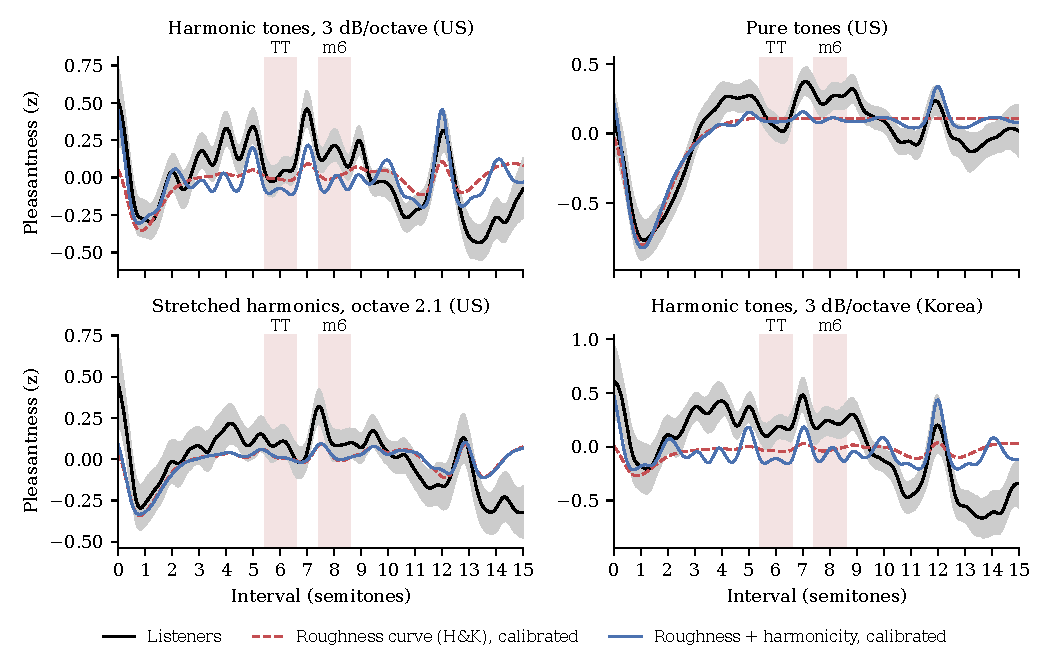
\includegraphics[width=\linewidth]{figures/fig_profiles.pdf}
\caption{Listener pleasantness profiles (black; grey band, 95\% bootstrap CI) with the
roughness curve (\HK, red dashed) and the roughness-plus-harmonicity curve (blue), each
calibrated to the listeners over all intervals outside the shaded windows at the tritone (TT)
and minor sixth (m6). Harmonic tones (top left); pure tones (top right); stretched partials
(bottom left); Korean listeners, harmonic tones (bottom right).}
\label{fig:profiles}
\end{figure}

\subsection{Roughness}
\label{sec:roughness}
Table~\ref{tab:gap} gives the gap in every experiment. For harmonic tones with a 3\,dB/octave
roll-off the minor sixth is rated \gapObsHarm\SDu{} \gapObsHarmCI{} above the tritone, and the
gap left by calibrated \HK{} roughness is \gapHKHarm\SDu{} \gapHKHarmCI. Pooled over the six US experiments
with harmonic spectra, the observed gap is \poolGapObsHarm\SDu{} \poolGapObsHarmCI{} and the
gap left by calibrated \HK{} roughness is \poolGapHKHarm\SDu{} \poolGapHKHarmCI, that is
\poolLeftHK\% of the observed gap (Table~\ref{tab:pooled}); the Sethares kernel leaves
\poolGapSethHarm. Between the fourth and the fifth the roughness curve is nearly flat, so once
calibrated it predicts almost the same pleasantness at the tritone and the minor sixth. Roughness separates the tritone from the fourth and fifth, whose low partials
coincide, but at the tritone and the minor sixth the near-miss pairs of partials that do
interact produce similar totals for these spectra. Its calibrated curve does reproduce the tritone's dip below the fourth and fifth in
part (pooled dip left \poolDipHKHarm, observed \poolDipObsHarm), which is why the dip and the
gap tell different stories. For
pure tones, whose partials do not interact at these intervals, roughness predicts no gap, yet
listeners produce one (\gapObsPure\SDu{} \gapObsPureCI).

\begin{table}[t]
\centering
\caption{The gap (minor sixth minus tritone), observed and left unexplained by each model
calibrated on the experiment itself, in within-listener SD [95\% participant-bootstrap CI].
Bold: CI excludes zero. The composite of \citet{marjieh2024} was fitted to these data.
$N$: participants.}
\label{tab:gap}
\footnotesize
\setlength{\tabcolsep}{4pt}
\resizebox{\linewidth}{!}{%
\begin{tabular}{lrcccc}
\toprule
& & & \multicolumn{3}{c}{Left unexplained after} \\
\cmidrule(lr){4-6}
Experiment & $N$ & Observed & Roughness & Roughness + harmonicity & Composite \\
\midrule
\tabinput{tables/tab_mj_gap.tex}
\bottomrule
\end{tabular}}
\end{table}

\subsection{Harmonicity closes the tritone's own shortfall}
\label{sec:harmonicity}
Adding harmonicity (published tolerance) leaves a pooled gap of \poolGapHKHHarm\SDu{}
\poolGapHKHHarmCI, \poolLeftHKH\% of the observed gap, with large heterogeneity
($I^2=\poolGapHKHHarmItwo\%$; Table~\ref{tab:pooled}). The primary estimand, the held-out gap
under the curve with a 20-cent tolerance, is \primGap\SDu{} \primGapCI{} ($\tau=\primTau$,
$I^2=\primItwo\%$). Three similar values in this paper answer different questions:
\primGap{} is the primary estimand (held out, 20-cent tolerance, random effects with a
Hartung--Knapp interval); \poolGapHKHHarm{} in Table~\ref{tab:pooled} is the descriptive
calibration, with the published tolerance and each experiment fitted to itself; and
\mbGapHKHtw{} in Section~\ref{sec:lodo} is the held-out gap of the 20-cent curve as a plain
mean over the six spectra. The primary estimand is a real gap, but the prediction interval for a new harmonic
spectrum, \primGapPI, includes zero, and per spectrum it ranges from \primNothree{} (five
harmonics without the third) to \primGuitar{} (guitar). The synthetic spectra leave little
(harmonic tones \primHarm, five equal harmonics \primEqfive); the resynthesised flute, guitar
and piano leave most (\primFlute, \primGuitar{} and \primPiano). Because the spectra we have
for those three instruments are proxies, this contrast may reflect spectral detail that the
models do not see as much as a property of the listeners.

The descriptive calibrations agree. Harmonicity without roughness leaves less of the gap
(\poolGapHHarm) but fits the rest of the interval axis worse: outside the excluded windows it
explains $R^2=\rfitHEqfive$, \rfitHNothree{} and \rfitHFlute{} of the profile for five equal
harmonics, five harmonics without the third and the flute, against \rfitHKHEqfive,
\rfitHKHNothree{} and \rfitHKHFlute{} for roughness plus harmonicity. The composite of
\citet{marjieh2024}, whose parameters were fitted to these experiments, leaves
\poolGapCompHarm, and harmonicity computed with \texttt{incon}'s template instead of Marjieh
et al.'s leaves \poolGapInconHarm. The dip is more sensitive to how harmonicity is weighted:
\poolDipObsHarm\SDu{} observed, \poolDipHKHHarm{} \poolDipHKHHarmCI{} after roughness and
harmonicity, \poolDipHHarm{} after harmonicity alone and \poolDipCompHarm{} after the composite
(Supplementary Table~\ref{S-tab:dip}). Since the dip compares the tritone with its immediate
neighbours, whereas the gap compares it with an interval on the other side of the fifth, the
two need not agree, and the next paragraph shows why they do not.

\paragraph{Which end of the gap?}
A gap is a difference, $r(8)-r(6)$, so it can arise at either end. Table~\ref{tab:ends}
splits it. Under roughness alone the tritone lies \rpfSixHK\SDu{} from its prediction and the
minor sixth \rpfEightHK; relative to the mean residual of the other intervals from the minor
second to the major seventh, the tritone is \rpfTTOtherHK{} below. The tritone's shortfall is
therefore relative, not reliably negative in absolute terms, and it is clearest for the
guitar, piano and five harmonics without the third. Adding harmonicity with the 20-cent
tolerance moves the tritone to \rpfSixTw{} and its difference from the other intervals to
\rpfTTOtherTw, neither distinguishable from zero, while the minor sixth stays at
\rpfEightTw. What is left of the gap is the minor sixth rated above the curve. The minor sixth
is not unusual in this: its residual does not differ from the mean of the minor and major
thirds, fourth, fifth and major sixth (\rpfMsixConsTw; Table~\ref{tab:resprofile}). These
residuals are relative to an intercept fitted on the rest of the interval axis, so they locate
where the shape of the curve is wrong, not absolute levels. The same holds for pure tones
(tritone \rpfPureTwSix, minor sixth \rpfPureTwEight; point estimates).

\begin{table}[t]
\centering
\caption{Which end of the gap. Held-out residuals (observed $-$ predicted) at the tritone,
$r(6)$, and the minor sixth, $r(8)$, under \HK{} roughness and under the recommended curve
(\HK{} + harmonicity, 20-cent tolerance), and the gap left by the latter, in SD
[participant-bootstrap CI]. Pooled row: random effects over the six harmonic spectra,
Hartung--Knapp CI; its last cell is the primary estimand. Bold: CI excludes zero.}
\label{tab:ends}
\footnotesize
\setlength{\tabcolsep}{3pt}
\resizebox{\linewidth}{!}{%
\begin{tabular}{lccccc}
\toprule
& \multicolumn{2}{c}{Roughness (\HK)} & \multicolumn{2}{c}{\HK{} + harmonicity (20 cents)} & \\
\cmidrule(lr){2-3}\cmidrule(lr){4-5}
Experiment & $r(6)$ & $r(8)$ & $r(6)$ & $r(8)$ & Gap left \\
\midrule
\tabinput{tables/tab_ends.tex}
\bottomrule
\end{tabular}}
\end{table}

\begin{table}[t]
\centering
\caption{Random-effects pooled estimates [95\% Hartung--Knapp CI] and 95\% prediction
intervals (PI) for a new experiment, SD units, with each model calibrated on the experiment
itself. Harmonic: the six US experiments with harmonic spectra. Eight: adds pure tones and
bonang. $^{a}$Fitted to these data. DerSimonian--Laird intervals: Supplementary
Table~\ref{S-tab:suppdl}.}
\label{tab:pooled}
\footnotesize
\setlength{\tabcolsep}{3.5pt}
\resizebox{\linewidth}{!}{%
\begin{tabular}{lcccccc}
\toprule
& \multicolumn{2}{c}{Gap, harmonic ($k=\kHarm$)} & \multicolumn{2}{c}{Gap, eight ($k=\kEight$)}
& \multicolumn{2}{c}{Dip, harmonic ($k=\kHarm$)} \\
\cmidrule(lr){2-3}\cmidrule(lr){4-5}\cmidrule(lr){6-7}
& Estimate [CI] & PI & Estimate [CI] & PI & Estimate [CI] & PI \\
\midrule
\tabinput{tables/tab_pooled.tex}
\bottomrule
\end{tabular}}
\end{table}

\begin{figure}[t]
\centering
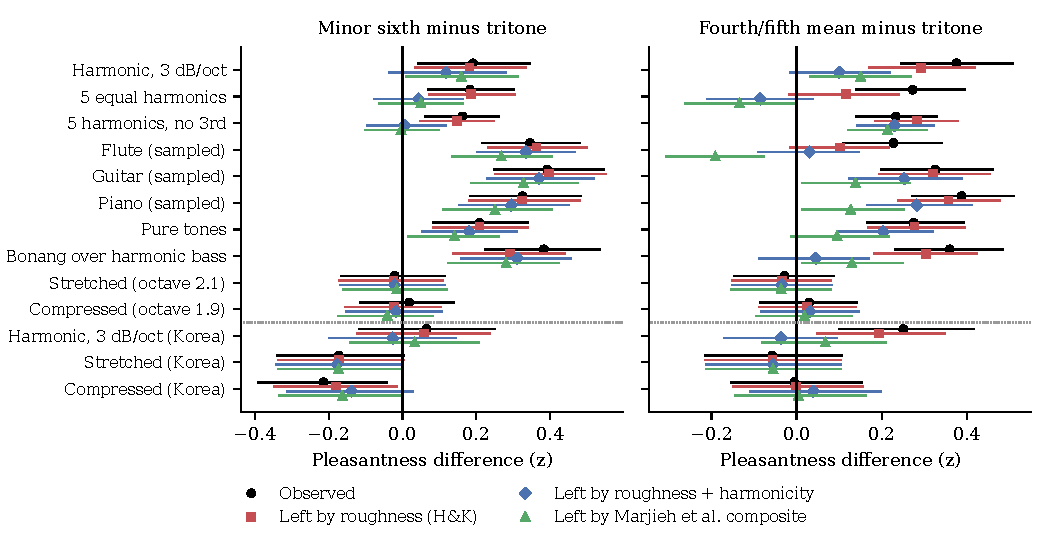
\includegraphics[width=\linewidth]{figures/fig_forest.pdf}
\caption{Observed gap and dip (black) and the part left unexplained by roughness (red),
roughness plus harmonicity (blue) and the fitted composite of \citet{marjieh2024} (green),
per experiment, each model calibrated on the experiment itself, with 95\% bootstrap CIs.
Below the dotted line: stretched and compressed spectra and the Korean cohort.}
\label{fig:forest}
\end{figure}

\paragraph{Tuning.}
Located with a narrower kernel (SD 0.1 semitones; exploratory), the listeners' minor-sixth
peak lies at \ejLocMsix{} cents, between equal temperament and 8/5 (\jiCentsMsix{} cents) and
\ejDiffMsix{} cents from the harmonicity model's peak, and the gap left is no smaller at
just-intoned positions (difference \ejGapJIaDiff), so these data cannot tell whether listeners
heard the minor sixth as tempered or just (inconclusive; Supplementary
Section~\ref{S-sec:etji}).

\subsection{A better curve on held-out spectra}
\label{sec:lodo}
With one pair of weights fitted across US experiments (published tolerance) and each
experiment predicted from weights fitted to the others (Table~\ref{tab:lodo}), the held-out
unexplained gap is positive in \lodoPos{} of \lodoN{} experiments and its CI excludes zero in
\lodoExcl; for harmonic spectra, in \lodoPosHarm{} and \lodoExclHarm{} of 6. The residual on
unseen spectra is in the same range as the descriptive one, so it is not an artefact of
refitting each experiment.

\paragraph{A pre-specified screen.}
Before looking, we fixed a list of candidate third factors, all computed from the stimulus and
none tied to a particular interval, and one criterion: prediction of held-out experiments.
The candidates were (1) a wider tolerance of mistuning in the harmonicity model, the Gaussian
width $\sigma$ of spectrum and template chosen from 6.83, 10, 15 or 20 cents inside each
fold; (2) root ambiguity \citep{terhardt1974,parncutt1988}, the height of the second-best peak
of the virtual-pitch profile relative to the best; (3) temporal periodicity, the largest
normalised autocorrelation of the partials over lags of 2--30\,ms \citep{pressnitzer2001},
in the spirit of \citet{stolzenburg2015} and \citet{masina2022}; and (4), as a deliberate
foil, the harmonic entropy of the frequency ratio \citep{erlich}, which ignores the spectrum.
Baselines were refitted inside each fold. The list was fixed in advance but not publicly
registered.

Only the tolerance helped (Table~\ref{tab:screen}). The fold-wise choice was
$\sigma=\scrChosenSigma$ cents in every fold, and the two-term curve then reaches a mean
held-out $R^2$ of \mbRtwoHKHtw, against \mbRtwoHKH{} with the published tolerance (paired
difference \mdRtwoTwVsHKH), \mbRtwoRev{} for revised roughness plus harmonicity and
\mbRtwoComp{} for the composite of \citet{marjieh2024} (paired difference \mdRtwoTwVsComp;
\mbNboot{} participant bootstraps of the whole leave-one-out procedure). The composite's
internal weights were fitted to these experiments, so the comparison favours it. Root
ambiguity ($R^2=\scrRtwoRA$) and periodicity ($R^2=\scrRtwoPER$) added nothing once
harmonicity was present, and the foil added nothing ($R^2=\scrRtwoHE$). Checked afterwards
(exploratory), the optimum depends on smoothing: with a kernel of 0.1 semitones the best
tolerance is \rbBestSigmaOne{} cents, with 10, 15 and 20 cents nearly tied (\rbRtwoOneTen,
\rbRtwoOneFifteen, \rbRtwoOneTwenty), and with 0.3 semitones it is \rbBestSigmaThree. A tolerance
wider than the published one helps at every width (gains \rbGainOne, \rbGainTwo{} and
\rbGainThree{} in $R^2$), but 20 cents is a representative value, not an estimate. Rows
examined after the screen are in Supplementary Table~\ref{S-tab:screenexpl}.

Before running the smoothing check we had set the criterion that the best tolerance
should lie within 15--25 cents at both the narrower and the wider kernel; it was met at 0.3
but not at 0.1 semitones, where some folds chose 10 cents. The lower tone of each dyad was
sampled from G3 to F4, whereas the models place it at C4; averaging \HK{} roughness over that
range changes the held-out $R^2$ of the recommended curve by \rbdRtwoRegVsHKHtw{} and harmonicity
is unaffected by transposition. Register does shift the overall liking of pure-tone dyads
\citep{kaklamani2025}, but a shift common to all intervals of an experiment is absorbed by its
intercept.

The tolerance improves the curve as a whole but barely moves the gap: the held-out gap in the
six harmonic experiments is \mbGapHKHtw\SDu, against \mbGapHKH{} with the published
tolerance, and no candidate removed it. Tolerance, ambiguity and periodicity together reach
$R^2=\scrRtwoAll$ and leave a gap of \scrGapAll. The residual is concentrated in pure tones
(\scrGapTwPure) and the resynthesised flute, guitar and piano (\scrGapTwFlute, \scrGapTwGuitar{}
and \scrGapTwPiano). The foil failed as intended on a second count: depending only on the
frequency ratio, it necessarily puts its penalty at 600 cents for stretched tones as well
(\scrHEpredDipSix\SDu{} in the fitted curve), where listeners show none
(Section~\ref{sec:tests}). With the dyads sampled continuously, a wider
tolerance means only that listeners' consonance peaks are broader than the model's; it is not
evidence about equal temperament as such (Section~\ref{sec:chords}).

\begin{table}[t]
\centering
\caption{Leave-one-experiment-out prediction (published tolerance). $b_R$, $b_H$: roughness
and harmonicity weights fitted to the other US experiments. Held-out unexplained gap and dip
[95\% CI], SD units. Bold: CI excludes zero.}
\label{tab:lodo}
\footnotesize
\setlength{\tabcolsep}{4pt}
\resizebox{\linewidth}{!}{%
\begin{tabular}{lrrccc}
\toprule
Held-out experiment & $b_R$ & $b_H$ & Gap, roughness only & Gap, two mechanisms & Dip, two mechanisms \\
\midrule
\tabinput{tables/tab_lodo.tex}
\bottomrule
\end{tabular}}
\end{table}

\begin{table}[t]
\centering
\caption{Pre-specified out-of-sample screen (leave one US experiment out; point estimates).
$R^2$: mean over held-out experiments of the fit to the whole profile (10 US; six harmonic).
Gap, dip: left unexplained, mean of the six harmonic experiments. TT $-$ other: the tritone's
residual dip minus the mean of the other 13 intervals (eight unstretched experiments).
Stretched: residual dip for stretched partials at 6.00 semitones and at the stretched scale's
tritone, 6.42. SD units. Post-hoc rows: Supplementary Table~\ref{S-tab:screenexpl}.}
\label{tab:screen}
\footnotesize
\setlength{\tabcolsep}{3pt}
\resizebox{\linewidth}{!}{%
\begin{tabular}{lccccccc}
\toprule
& \multicolumn{2}{c}{Held-out $R^2$} & & & & \multicolumn{2}{c}{Stretched, dip left} \\
\cmidrule(lr){2-3}\cmidrule(lr){7-8}
Model & 10 US & 6 harm. & Gap left & Dip left & TT $-$ other & at 6.00 & at 6.42 \\
\midrule
\tabinput{tables/tab_screen.tex}
\bottomrule
\end{tabular}}
\end{table}

\begin{figure}[t]
\centering
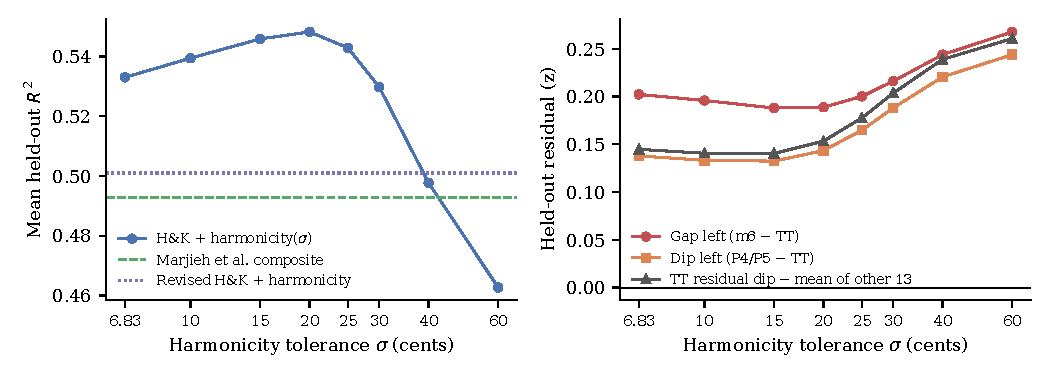
\includegraphics[width=\linewidth]{figures/fig_sigma.pdf}
\caption{Harmonicity tolerance. Left: mean held-out $R^2$ of roughness plus harmonicity as
the Gaussian width $\sigma$ varies (published value 6.83 cents), against revised roughness
plus harmonicity and the composite of \citet{marjieh2024}. Right: the tritone residuals left
on held-out harmonic experiments. Values beyond 20 cents were examined after the screen.}
\label{fig:sigma}
\end{figure}

\subsection{Is the tritone special?}
\label{sec:special}
Table~\ref{tab:resprofile} gives the held-out residual at every integer interval, pooled by
random effects over the six harmonic spectra. Under roughness alone the most negative residuals
between the minor second and the major seventh are those of the major second
(\rpfMajSecHK) and the tritone (\rpfSixHK). After harmonicity with the 20-cent tolerance the
consonant intervals, thirds, fourth, fifth and sixths, lie above the curve (the minor third
\rpfMinThirdTw, fourth \rpfFourthTw, fifth \rpfFifthTw, major sixth \rpfMajSixthTw), while the
seconds, the tritone and the minor seventh lie near it (tritone \rpfSixTw, major second
\rpfMajSecTw, minor seventh \rpfMinSevTw) and the major seventh lies above it
(\rpfMajSevTw). The tritone is thus one of several intervals that the
curve predicts about right, not an interval detectably rated below it. Measured instead as a dip below its
two neighbours, the tritone's dip after harmonicity (published tolerance) differs from that
of the average interval by \ttoHKHHarm{} \ttoHKHHarmCI{} over the six harmonic spectra, an
interval that includes zero, but by \ttoHKHEight{} \ttoHKHEightCI{} when pure tones and the
bonang are added; under the composite of \citet{marjieh2024} the eight-spectrum figure is
\ttoCompEight{} \ttoCompEightCI. These intervals are for the published tolerance; for the
20-cent curve only point estimates are available (Table~\ref{tab:screen}). We report the
eight-spectrum figure rather than drop it. Since the tritone's own
residual is not below average, that excess reflects the fourth and fifth rated above the curve
on either side, not a shortfall at the tritone. Per-interval dips are shown in Supplementary Figure~\ref{S-fig:null}.

\begin{table}[t]
\centering
\caption{Held-out residual (observed $-$ predicted) at each integer interval, random effects
over the six harmonic US spectra, SD units. $^*$Hartung--Knapp CI excludes zero. Size:
a linear term in interval size (Section~\ref{sec:ceiling}).}
\label{tab:resprofile}
\scriptsize
\setlength{\tabcolsep}{2pt}
\resizebox{\linewidth}{!}{%
\begin{tabular}{lcccccccccccccc}
\toprule
Model & m2 & M2 & m3 & M3 & P4 & TT & P5 & m6 & M6 & m7 & M7 & P8 & m9 & M9 \\
\midrule
\tabinput{tables/tab_resprofile.tex}
\bottomrule
\end{tabular}}
\end{table}

\paragraph{A bonus for in-tune intervals and a step (exploratory).}
Two further patterns were found after seeing the residual profile. Both are computed on the
held-out residual of the curve with the 20-cent tolerance and a linear term in interval size
(which absorbs the smooth trend of Section~\ref{sec:ceiling}). The first is a local bonus: the
residual at an equal-tempered interval $c$ minus the mean at the quarter-tones on either side,
$b(c)=r(c)-[r(c-0.5)+r(c+0.5)]/2$. Pooled over the harmonic spectra, the intervals from the
minor second to the major seventh other than the tritone have a mean bonus of
\decTwoBonusOther\SDu{} and the tritone \decTwoBonusTT; the individual bonuses run from
\decTwoBMinSev{} (minor seventh) and \decTwoBMajSec{} (major second) to \decTwoBMajThird{}
(major third). The tritone's shortfall relative to the other intervals, \decTwoOtherMinusTT,
includes zero. What the data do separate, and what we noticed only after seeing the profile,
is that the major second and minor seventh receive a smaller bonus than the other eight
intervals (\decTwoMMvsRest, $I^2$ near zero); the tritone does not differ from them
(\decTwoTTvsMM). The minor second and the major seventh, which are rougher, receive the
full bonus, and we do not know what separates the three intervals with a smaller one.

The bonus belongs to harmonic tones. Computed in the same way on the curve with a sharpness
term (Section~\ref{sec:ceiling}), it is \gbSharpHarmOther{} for harmonic spectra but
\gbSharpPure{} for pure tones and \gbSharpBonang{} for the bonang, and at either scale of the
stretched and compressed tones it is not distinguishable from zero
(Section~\ref{sec:tests}). It survives changes of the harmonicity model: fitting two
harmonicity terms of different width leaves most of it, and so do the published tolerance and
Marjieh et al.'s revised roughness, which makes the slow beats of slightly mistuned intervals
pleasant. At a smoothing width of 0.2 semitones the bonus cannot tell equal temperament from
just intonation, so we read it as a bonus for the neighbourhood of the familiar intervals, not
for their exact tuning. \citet{marjieh2024} noted that details of the timbral effects remain
unexplained by their models; we are not aware that this bonus has been quantified.

The second pattern is a step. Writing $r(c)=b(c)+q(c)$, with $q(c)$ the mean residual at the
two neighbouring quarter-tones, the gap splits into a bonus part, $b(8)-b(6)$, of
\decTwoBonusPart, and a baseline part, $q(8)-q(6)$, of \decTwoBasePart; the baseline rises
between 7 and 8 semitones by \decTwoStep{} as an indicator after a linear trend
($I^2=\decTwoStepItwo\%$). On plain means over the spectra both parts exclude zero
(\decTwoBonusPartFixed{} and \decTwoBasePartFixed), but under random effects only the baseline
part does, and the split is not stable across spectra (Table~\ref{tab:decomp}). The step is
absent for the synthetic harmonic tone (\decTwoStepHarm) and the flute (\decTwoStepFlute), and
large for the guitar (\decTwoStepGuitar) and piano (\decTwoStepPiano). The guitar and piano
spectra are proxies, one analysed tone each, so the step may come from the spectral model
rather than from the listeners. The step is robust to the kernel width, the exclusion window
and binning (Supplementary Table~\ref{S-tab:step}); what it is not robust to is the spectrum.
We therefore do not decompose the gap into a fixed share of step and bonus.

\begin{table}[t]
\centering
\caption{Decomposition of the held-out gap (exploratory; \HK{} + harmonicity at 20 cents +
interval size), per harmonic spectrum [participant-bootstrap CI] and pooled by random effects
[Hartung--Knapp CI]. Bonus part $b(8)-b(6)$; baseline part $q(8)-q(6)$; step: baseline rise
between 7 and 8 semitones after a linear trend; other $-$ TT: mean bonus of the other
intervals minus the tritone's. Bold: CI excludes zero. Guitar and piano use proxy spectra.}
\label{tab:decomp}
\footnotesize
\setlength{\tabcolsep}{3pt}
\resizebox{\linewidth}{!}{%
\begin{tabular}{lccccc}
\toprule
Spectrum & Gap left & Bonus part & Baseline part & Step & Other $-$ TT bonus \\
\midrule
\tabinput{tables/tab_decomp_spectra.tex}
\bottomrule
\end{tabular}}
\end{table}

\subsection{What the residual depends on}
\label{sec:tests}

\paragraph{Spectrum.}
With stretched or compressed partials the unexplained gap at 600 cents is about zero (US,
after roughness and harmonicity: \gapHKHStr{} and \gapHKHComp\SDu), and so is the observed
dip (\dipObsStr{} and \dipObsComp), although the profiles are not flat (profile SD
\profSDStr{} and \profSDComp, against \profSDHarm{} for harmonic tones). A penalty attached
to the physical 600-cent interval would survive stretching, since the fundamentals are still
600 cents apart. With partials stretched to an octave ratio $r$, the scale that matches the
spectrum has its tritone at $6\log_2 r$ semitones: \sscPosStr{} for the stretched and
\sscPosComp{} for the compressed tones. There the stretched tones show an observed dip of
\sscObsDipStr\SDu, where there was none at 6 (paired difference \sscObsDipStrDiff). Held-out
\HK{} roughness predicts a dip of \mbStrPredHK{} at that position and leaves \mbStrSscHK{}
\mbStrSscHKCI; the foil, attached to the frequency ratio, necessarily puts its penalty at 600
cents instead. For compressed tones the dip at \sscPosComp{} is not significant
(\sscObsDipComp), and the Korean listeners show no clear dip at either position, so the
shift rests on one spectrum and one cohort.

The in-tune bonus of Section~\ref{sec:special} does not follow the stretched scale. At the
stretched scale's own intervals the mean bonus is \sbOwnStr{} (compressed \sbOwnComp), against
\sbOwnHarm{} for harmonic tones, and the minimum effect these data could detect with 80\%
power is \sbMdeStr\SDu{} (Supplementary Table~\ref{S-tab:strbonus}; exploratory). The Korean
listeners show the same pattern (harmonic \sbOwnHarmKr, stretched \sbOwnStrKr). The dip moves
with the partials; the bonus stays with harmonic tones.

The published harmonicity model cannot follow the shifted dip, because its template is a
harmonic series. Replacing the template with the upper tone's own partials, one reading of the
proposal that harmonic templates are learned from the sounds heard \citep{shamma2000},
reproduces the stretched-scale dip but predicts harmonic tones worse, so it is not a better
general curve (exploratory; Supplementary Section~\ref{S-sec:timbrerel}).

\paragraph{Targeted tests.}
Four contrasts, fixed in advance, probe the residual after roughness and harmonicity
(Table~\ref{tab:holm}); the Holm correction over them was added in this version. Korean minus US listeners, same harmonic stimuli: \holmEstCulture{}
($p=\holmPCulture$). Musicians (more than two years of training) minus non-musicians, pooled
over the eight unstretched US experiments: \holmEstMus{} ($p=\holmPMus$). Five harmonics
without the third minus with it, observed change in the dip minus the change predicted by
roughness (\nthreeHKDip): \holmEstThird{} ($p=\holmPThird$). The change in the gap from 2 to
12\,dB/octave roll-off, observed minus roughness-predicted: \holmEstRoll{} ($p=\holmPRoll$).
After Holm correction \holmNsurvive{} of the four remain significant (adjusted $p$ from
\holmPadjThird{} to \holmPadjRoll).

Taken individually, the contrasts say the following. Musicians show a larger observed gap and
dip (\musPoolGap{} and \musPoolDip; Table~\ref{tab:tests}), part of which follows from
harmonicity, to which musicians are more sensitive \citep{mcdermott2010}. After roughness and
harmonicity the gap is \grpMusGapHKH{} for musicians and \grpNonGapHKH{} for non-musicians,
and the differences include zero (gap \musPoolGapHKH, dip \musPoolDipHKH), so the data do
not establish a larger residual in trained listeners; the residual is present in
non-musicians. For stretched and compressed partials the groups do not differ (gap difference
\musPoolStrGap; fixed-effect pooling over two experiments). Korean listeners show a smaller
gap for harmonic tones, but they differ from US listeners in the same direction for stretched
and compressed partials (\cohObsGapStr{} and \cohObsGapComp), where US listeners show no gap,
so the difference is not specific to consonance. Removing the third harmonic changes the
observed dip less than roughness predicts (observed change \nthreeObsDip), consistent with
\citet{marjieh2024}, who found that the third harmonic matters through harmonicity; after
correction this is suggestive only. In the roll-off experiment the gap is \rollTwoGap,
\rollSevenGap{} and \rollTwelveGap\SDu{} at 2, 7 and 12\,dB/octave, while calibrated roughness
predicts \rollTwoHKpred, \rollSevenHKpred{} and \rollTwelveHKpred: the gap does not shrink as
the upper partials, and with them the roughness, fade (Supplementary
Table~\ref{S-tab:rolloff}).

\paragraph{Culture and the smooth trend.}
The models fit the Korean profiles poorly (roughness plus harmonicity, in-sample
$R^2=\profRfitHarmKr$ for harmonic tones), although their ceilings are high
(\krCeilMin--\krCeilMax). Predicted with weights from US listeners, the recommended curve
does worse than each experiment's mean (held-out $R^2$ \krHoTw{} on average); adding a linear
term in interval size brings it to \krHoSize{} and a sharpness proxy to \krHoSharp
(Supplementary Table~\ref{S-tab:korean}; exploratory). What separates the cohorts in these
data is thus mainly a steeper decline of pleasantness with interval size, not a different
ordering of consonances. Its cause is open: sharpness, which rises with interval size, is one
candidate, and in an online study so is the playback equipment, which may differ between
cohorts.

\begin{table}[t]
\centering
\caption{The four pre-specified targeted tests, on the residual after roughness and
harmonicity (published tolerance). SE from the participant bootstrap (musicianship: random
effects over eight experiments, Hartung--Knapp SE, $t$ on 7 df). $p$: two-sided;
Holm: adjusted over the four.}
\label{tab:holm}
\footnotesize
\begin{tabular}{p{0.56\linewidth}rrrr}
\toprule
Contrast & Estimate & SE & $p$ & Holm $p$ \\
\midrule
\tabinput{tables/tab_holm.tex}
\bottomrule
\end{tabular}
\end{table}

\begin{table}[t]
\centering
\caption{Differences between groups [95\% bootstrap CI], SD units. Musicianship rows give the
number of musicians/non-musicians. Bold: CI excludes zero (uncorrected).}
\label{tab:tests}
\footnotesize
\setlength{\tabcolsep}{4pt}
\resizebox{\linewidth}{!}{%
\begin{tabular}{lcccc}
\toprule
& Observed gap & Gap after rough.\ + harm. & Observed dip & Dip after rough.\ + harm. \\
\midrule
\tabinput{tables/tab_tests.tex}
\bottomrule
\end{tabular}}
\end{table}

\subsection{Chords}
\label{sec:chords}
Scored in equal temperament, as in \texttt{incon} and in earlier analyses, including one by the author, the
twelve Bowling dyads show the pattern of the dense data (Table~\ref{tab:bowling}): roughness
reproduces \bshareHKET\% of the tritone--minor-sixth difference and roughness plus harmonicity
\bshareHKHET\%. In the chords, each tritone costs \bpenSizeET{} rating units with only chord
size controlled and \bpenHKHET{} \bpenHKHETCI{} after roughness and harmonicity. But the
chords were played in just intonation. At the presented tuning, harmonicity rates the minor
sixth (8/5) higher (\harmJIMsix{} against \harmETMsix{} in equal temperament), while the
tritone (7/5) barely changes (\harmJITT{} against \harmETTT). Scored as presented, roughness
plus harmonicity reproduces \bshareHKHJI\% of the dyad difference and the chord-level tritone
penalty falls to \bpenHKHJI{} \bpenHKHJICI. With twelve dyads the share is an overfit-prone
statistic; the chord-level penalty, estimated from \bNTT{} chords containing a tritone, is the
firmer result.

The Johnson-Laird chords were equal-tempered, and there a penalty remains: \jpenHKH{}
\jpenHKHCI{} rating units per tritone after roughness and harmonicity (rating SD
\jRatingSD), and \jpenHKHF{} \jpenHKHFCI{} with familiarity added. Those chords are widely
voiced and were rated by a different population, so the two sets are not directly
comparable. The 20-cent tolerance reduces the Johnson-Laird penalty to \csJLTwenty{}
\csJLTwentyCI{} (paired difference \csJLDiff), no longer distinguishable from zero, and fits the just-intoned Bowling chords worse
($R^2$ \csBJISevenRtwo{} to \csBJITwentyRtwo), so the tolerance that suits listeners depends on
the tuning they hear. Rescoring the Bowling chords also changes the unique variance of
harmonicity relative to interference and familiarity: with chord size controlled it rises
from \dRBSizeH{} to \dRBjiSizeH, comparable to the other two, and the full model's $R^2$ rises
from \RfullBSize{} to \RfullBjiSize. Without a chord-size control familiarity appears to
dominate, as an earlier analysis by the author reported (Supplementary
Table~\ref{S-tab:chorddecomp}).

\begin{table}[t]
\centering
\caption{\citet{bowling2018}: share (\%) of the tritone--minor-sixth dyad difference
reproduced by each fitted model (12 dyads), and the tritone penalty in chords (rating units
per tritone, chord size controlled [95\% CI]; $n=298$), with the models scored at
equal-tempered (ET) or the presented just-intoned (JI) pitches.}
\label{tab:bowling}
\footnotesize
\setlength{\tabcolsep}{4pt}
\begin{tabular}{lcccc}
\toprule
& \multicolumn{2}{c}{Dyad share (\%)} & \multicolumn{2}{c}{Chord tritone penalty} \\
\cmidrule(lr){2-3}\cmidrule(lr){4-5}
Model & ET & JI & ET & JI \\
\midrule
\tabinput{tables/tab_bowling_ji.tex}
\bottomrule
\end{tabular}
\end{table}

\subsection{How much the curves miss overall}
\label{sec:ceiling}
The split-half ceilings range from \ceilMin{} to \ceilMax{} (US mean \ceilUS). Held out, the
recommended curve captures \shBaseFrac\% of the explainable variance in the US experiments and
the composite of \citet{marjieh2024} \shCompFrac\%. The shortfall is not at the tritone. Fitted
to single experiments, the residuals share a broad shape: intervals in the middle of the range
are rated above the curve and wide intervals, above all beyond the octave, below it. A linear
term in interval size removes most of this (in-sample $R^2$ \insBaseHarmThree{} to
\insXHarmThree{} for harmonic tones, and a Korean mean of \insBaseKR{} to \insXKR). Its slope
depends on the spectrum: \slopeHarmThree\SDu{} per octave of interval for harmonic tones and
\slopePure{} for pure tones, but \slopeEqFive{} for five equal harmonics and \slopeFlute{} for
the flute; for Korean listeners \slopeKrMax{} to \slopeKrMin. Interval size is confounded here
with the pitch of the upper tone and with sharpness, the weighting of a spectrum towards high
frequencies \citep{zwicker2007}. Sharpness was a component of sensory pleasantness in
psychoacoustics \citep{aures1985} before consonance models narrowed to roughness and
harmonicity, it lowers the consonance of chords in high registers \citep{eerola2022register},
and for pure-tone dyads preference falls as mean frequency rises \citep{kaklamani2025}.

As an exploratory comparison, chosen after seeing the residuals, we added one smooth term
with a weight shared by all experiments. Held-out US $R^2$ rises from \shBaseRtwoUS{} to
\shXRtwoUS{} with interval size and to \shSharpRtwoUS{} with a sharpness proxy computed from
the synthesis parameters (paired difference \shdRtwoUSVsBase), that is from \shBaseFrac\% to
\shSharpFrac\% of the explainable variance; widening the tolerance, by comparison, added
\shTolGain. Sharpness's edge over interval size is the part that selection may have produced.
The gain does not depend on the roughness model: with Marjieh et al.'s revised
roughness the US $R^2$ rises from \shRevRtwoUS{} to \shRevSharpRtwoUS. It is concentrated in the
synthetic spectra (harmonic tones \shBaseRtwoHarmThree{} to \shSharpRtwoHarmThree, stretched
\shBaseRtwoStr{} to \shSharpRtwoStr), and two spectra do not fit it: for five equal harmonics
the trend is absent although sharpness rises with the interval, and the flute, whose ratings
rise with interval size, loses (\shBaseRtwoFlute{} to \shSharpRtwoFlute). The roll-off
experiment, which varied the spectral slope across the trials of the same participants, offers
a check within listeners, although we looked at it before choosing sharpness. Fitted
separately at each roll-off, the slope over interval size flattens from \roSlopeOne{} at
1\,dB/octave to \roSlopeThirteen{} at 13, as sharpness predicts and interval size alone does
not, but the proxy's implied slopes cover only \roImpShare\% of that flattening. Finally, for
the one rating set of \citet{marjieh2024} not yet analysed, \ctNChords{} triads of five equal
harmonics rated by \ctNPart{} participants, we wrote down three predictions before reading the
data: a negative sharpness weight, a better leave-one-chord-out $R^2$, and a better
correlation of the frozen-weight curve with the chord means. None passed (weight \ctBS;
$R^2$ difference \ctLooDiff; correlation difference \ctRDiff; Supplementary
Section~\ref{S-sec:sharpness}), although the triads leave little room for a third term. We therefore treat the smooth trend as established and
sharpness as a candidate explanation, and we do not add it to the recommended curve.

\begin{figure}[t]
\centering
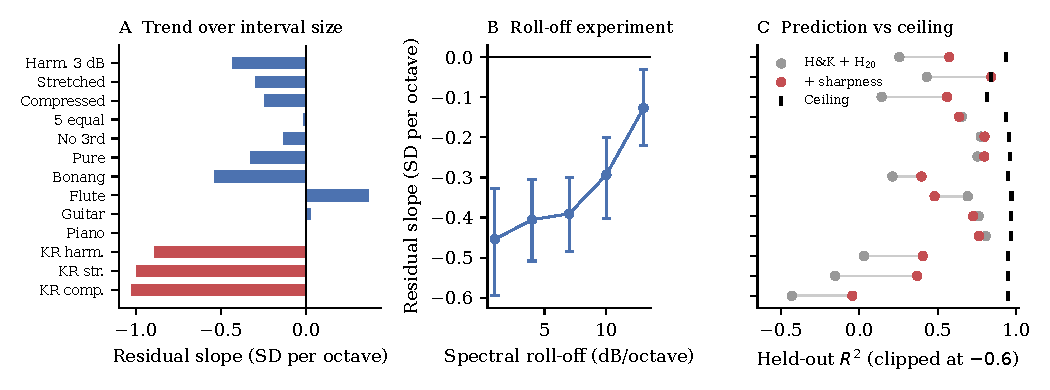
\includegraphics[width=\linewidth]{figures/fig_sharp.pdf}
\caption{The smooth trend (exploratory). (A) Slope over interval size of the residual from
\HK{} roughness plus harmonicity (20-cent tolerance), each experiment fitted alone (SD per
octave of interval). (B) The same slope in the roll-off experiment at each spectral roll-off
(participant-bootstrap 95\% CI). (C) Held-out $R^2$ per experiment without and with the
sharpness term, against the split-half ceiling (Korean experiments predicted with weights
from all US experiments).}
\label{fig:sharp}
\end{figure}

% =====================================================================
\section{Discussion}

\subsection{What closes the gap, and the recommended curve}
\label{sec:curve}
For harmonic tones and US listeners the minor sixth is rated \poolGapObsHarm{}
within-listener SD above the tritone, and a roughness curve calibrated on the
rest of the interval axis predicts none of it: roughness is almost flat between the fourth and
the fifth. The popular diagnosis, that the dissonance curve is an oversimplification, is
correct in a precise sense. What is missing is harmonicity. The tritone's partials fit no
single harmonic series well, whereas those of the minor sixth approximate the series whose 5th
and 8th harmonics are the two fundamentals. With harmonicity in the curve the tritone's own
shortfall is no longer detectable, and root ambiguity, periodicity and harmonic entropy add nothing: an
interval whose partials fit no single series is the same interval whose virtual pitch is
ambiguous.

The curve we recommend is
$P(x)=\alpha_e+b_R\,R_{\mathrm{HK}}(x)+b_H\,H_{20}(x)$, with $R_{\mathrm{HK}}$ the
Hutchinson--Knopoff roughness of the dyad's combined spectrum, $H_{20}$ Harrison and Pearce's
harmonicity computed with a 20-cent tolerance (11-harmonic template weighted $1/i$, the same
Gaussian width for spectrum and template, lower tone at C4), both smoothed with the
0.2-semitone kernel, and pooled weights $b_R=\scrBetaR$ and $b_H=\scrBetaH$ for the 20-cent
curve (per unit of each raw model output; $\alpha_e$ is an experiment intercept). It has no
interval-specific term. It predicts held-out US experiments better than the published
combinations we tested, but only slightly better than the same curve with the published
tolerance; for just-intoned tones the published tolerance fits better. Neither the curve
family nor its ingredients are new \citep{parncutt2019,harrison2020,marjieh2024,masina2022};
what is new is that its tritone predictions were tested on experiments not used to fit it,
against candidates fixed in advance, and on a spectrum that moves the intervals.

Three cautions apply to anyone who uses it. First, its weights are for new spectra of the kind
tested here; on the experiments themselves they were refitted without the experiment being
predicted, and the intercept makes the curve a statement about the shape of the profile, not
its level. Second, the tolerance is a smoothing choice as much as a psychoacoustic parameter,
since it interacts with the kernel that smooths ratings and model outputs alike; at a finer
resolution the 20-cent curve smooths away the minor-sixth peak that listeners show
(Supplementary Section~\ref{S-sec:etji}). Third, the
curve is meant for equal-tempered tones; chords presented in just intonation should be scored
as presented and with the published tolerance. A smooth term over interval size would improve
it more than anything tested at the tritone, but until its cause is known we leave it out.

\subsection{What remains, and how to read it}
\label{sec:discussion-remains}
What remains in dyads is the primary estimand, \primGap\SDu{} \primGapCI, about
\poolGapHKHHarmRaw{} points on a seven-point scale for the descriptive calibration. It is not
a constant in three respects. It varies between spectra more than sampling error allows
(prediction interval \primGapPI), with the largest values for the proxy spectra of the
sampled instruments. It is absent at 600 cents when the partials are stretched or
compressed. And it is not detectably the tritone's: after harmonicity the tritone's residual does not
differ from zero, and
the minor sixth above it, like the other consonances. The exploratory decomposition does not
change this. Its step is carried by two proxy spectra, and the tritone's reduced in-tune bonus
does not separate it from the other intervals once spectra are treated as a random sample; the
one contrast that is clear, a smaller bonus for the major second and minor seventh, was found
after seeing the profile. We would not add a tritone penalty to a dissonance model. We would add
harmonicity and look for what makes consonant intervals of harmonic tones more pleasant than
any current curve predicts.

\paragraph{Pure tones.}
Pure tones might seem to cut the other way: they have no upper partials to align, yet they
leave one of the largest gaps. The residual profile resolves this. For pure tones the tritone
is predicted about right (\rpfPureTwSix) and the gap is the minor sixth (\rpfPureTwEight), so
pure tones give no evidence of a penalty at 600 cents in the first place. Because their
partials are the fundamentals, pure tones cannot separate spectral accounts from accounts
based on the frequency ratio; only a spectrum whose partials depart from the harmonic series
can.

\paragraph{The stretched tones and the heard octave.}
With stretched partials the dip leaves 600 cents and appears at the stretched scale's tritone.
An earlier analysis by the author read this as compatible with a learned category defined
relative to the octave the listener actually hears. That reading predicts more than the dip:
a category re-centred on the heard octave should also carry the in-tune bonus to the
stretched scale's intervals. It does not (\sbOwnStr, with a detectable effect of
\sbMdeStr, against \sbOwnHarm{} for harmonic tones). The dip follows the partials and the bonus
does not, which favours a spectral account of the dip, in which partials of the two tones
line up or fail to, over a re-centred learned category. This fits the finding that
consonance judgements for inharmonic bell timbres follow their partials rather than the
nominal intervals \citep{harrison2024carillon}. It rests on one stretched spectrum; the
compressed tones show no clear dip at their own tritone.

\paragraph{Two readings of the minor-sixth residual.}
The first is that the harmonicity model is incomplete. The tuning analysis does not identify
the defect: the listeners' minor-sixth peak lies between equal temperament and just
intonation, and the gap is no smaller at just-intoned positions. A harmonicity model wrong in
some other detail would have to explain why the residual varies between spectra, why it is
shared by the other consonant intervals, why it vanishes in the just-intoned Bowling chords
and why a penalty persists in the equal-tempered Johnson-Laird chords. The second reading is
learned: familiarity with the consonant intervals of tonal music, heard mostly in harmonic
sounds \citep{lahdelma2022,mcdermott2016}. The in-tune bonus fits this reading, since it
appears for harmonic tones and not at either scale of the stretched and compressed ones. But
the targeted tests do not support its usual corollaries once corrected for multiplicity:
neither training \citep[compare][]{mcdermott2010,popescu2019} nor culture
changes the residual detectably. These two readings are those of the current debate, between
psychoacoustic accounts in which harmonicity is a perceptual mechanism
\citep{harrison2020,marjieh2024} and the view that harmonicity partly stands in for exposure
\citep{lahdelma2022,milne2023}. Our data locate the residual at consonant intervals of harmonic
tones; they cannot tell which reading is right.

The chords sharpen the contrast without resolving it. The just-intoned Bowling chords leave
no tritone penalty after roughness and harmonicity, and the equal-tempered Johnson-Laird
chords leave one, which the 20-cent tolerance reduces to a value whose interval includes
zero (\csJLTwenty{} \csJLTwentyCI). This is what an
incomplete harmonicity model would produce if it under-credits equal-tempered consonances,
and it is also what a learned preference for familiar equal-tempered intervals would produce.
The two chord sets differ in voicing and population as well as tuning, and in chords the
tritone penalty is estimated from a count of tritones, so the chords do not show that the
tritone is special either; they show that tuning must be scored as presented.

\paragraph{What would decide.}
Three experiments would separate the readings. A replication of the stretched-spectrum result
with a second stretch factor and a second cohort would test whether the dip follows the
partials generally, and a dense sampling of the minor-sixth and major-third regions at a
resolution finer than the 14 cents that separate the two tunings, with enough listeners per
spectrum, would locate the peaks well enough to decide whether the harmonicity model
mis-places them. A comparison of listeners with little exposure to equal-tempered harmonic
music, rating the same dense dyads, would test the learned reading directly; the Korean
cohort here is too small and too different in recruitment to do so. Finally, the dip and the
gap should be measured in musical context, where the tritone's reputation was formed: the
isolated dyads here say how a tritone sounds, not how it functions.

\subsection{What dissonance curves can say}
Roughness curves computed from measured instrument spectra do not settle the ordering of the
tritone and the minor sixth. Across eight instruments at C4 and four kernels, the instrument
accounts for \shareInstrNoV\% of the variance of the tritone/minor-sixth roughness difference,
the kernel for \shareModelNoV\% and their interaction for \shareInterNoV\%; the rarely reported
shape constants of the \HK{} kernel move it by a median \sensABNarrowMed\pp, and one clarinet
spectrum reverses the listeners' ordering under \HK{} in two libraries (Supplementary
Section~\ref{S-sec:measured}). Combined with the finding that listeners do not follow roughness in
this region even for idealised spectra, roughness curves should not be used to argue about
the tritone either way. We recommend that analyses report the kernel and its constants, the
partial-merging and peak-acceptance rules, the recording and register, the tuning at which
the stimuli were presented, and whether the conclusion holds for a second recording; and that
any new curve be judged on held-out spectra and against the noise ceiling, not against the
previous curve.

% =====================================================================
\section{Limitations}
The dense data are online pleasantness ratings of synthetic or resynthesised dyads heard in
isolation; the tritone's reputation concerns musical context, which these data do not reach.
For the flute, guitar and piano the spectra are proxies from one analysed tone, and the
largest residuals, and the step of the exploratory decomposition, are found there. Models were
evaluated with the lower tone at C4, whereas it was sampled from G3 to F4; averaging roughness
over that range changes the held-out $R^2$ of the recommended curve by \rbdRtwoRegVsHKHtw{} and its dip by \rbdDipRegVsHKHtw. Six harmonic experiments are few
for estimating heterogeneity, which is large; Hartung--Knapp intervals are wider than the
DerSimonian--Laird intervals reported earlier, and \reNflip{} of \reNest{} pooled estimates
change whether they exclude zero. Experiments are treated as independent although some
participants may have taken part in more than one. The primary estimand was declared in this
version, after the author's earlier analyses, although the question and the curve were fixed before;
the screen's candidate list was fixed in advance but not publicly registered. The in-tune
bonus, the step, the residual profile, the stretched-scale bonus, the tuning analysis, the
sharpness term and the Korean held-out fits are exploratory. The four targeted tests are
corrected for multiplicity; the many other contrasts are not. The stretched-scale results rest
on one spectrum and one cohort, and the test of the heard-octave account assumes that a
re-centred category would carry the bonus as well as the dip. The tuning analysis could not
separate equal temperament from just intonation: the peak's interval spans both, and
equivalence was not shown (Supplementary Section~\ref{S-sec:etji}). The Korean cohort is small,
differs from the US cohort in recruitment and playback equipment as well as culture, and its
profiles are poorly fitted. The musicianship split is observational with a coarse two-year
threshold. Roughness here is a model quantity, not a measured percept \citep{mcbride2025}. The
Bowling analysis rests on twelve dyads and 298 chords from 30 listeners; the chord bootstraps
resample chords, not raters; and the Johnson-Laird chords differ in voicing, tuning and
population. The sharpness proxy is computed from synthesis parameters, was chosen after seeing
the residuals and failed its pre-specified (not publicly registered) triad test. No new listener data were collected.

% =====================================================================
\section{Conclusion}
Listeners rate the tritone below the minor sixth, and a roughness curve explains none of that.
A curve with harmonicity added, tolerating more mistuning than the published model, predicts
held-out experiments slightly better than published curves and leaves a gap of \primGap{}
within-listener SD \primGapCI{} that varies between spectra and is unexplained. That gap sits
at the minor sixth, which listeners rate above the curve as they do the other consonances; the
tritone's own residual does not differ detectably from zero. With stretched partials the tritone's dip follows the
partials, and none of the tests of training, culture, third harmonic or roll-off survives
correction. The larger failure of dissonance curves is a smooth trend over interval size,
which leaves them far below the reliability of the ratings. In dyads, harmonicity
accounts for the shortfall, and what remains is not detectably the tritone's.

\section*{Acknowledgements}
I thank Dr. Zoe Lin ([TITLE], [DEPARTMENT], [UNIVERSITY]) for supervising my summer research
and advising on the research approach. Any errors are my own.

\section*{Data availability}
No new data were collected; the study reanalyses published data. The dense dyad ratings and
timbre parameters are from \citet{marjieh2024code}
(\url{https://gitlab.com/pmcharrison/timbre-and-consonance-paper}), the chord ratings from
\citet{dcmlab} (\url{https://github.com/DCMLab/consonance}) and \citet{incondata}
(\url{https://github.com/pmcharrison/inconData}), and the instrument recordings from
\citet{philharmonia} (\url{https://philharmonia.co.uk/resources/sound-samples/}) and
\citet{iowamis} (\url{https://theremin.music.uiowa.edu/MIS.html}). The code repository provides
scripts that fetch these data rather than copies; the partials extracted from the recordings are
included as derived data.

\section*{Code availability}
All analysis code, intermediate results and the manuscript source are available at
\url{https://github.com/boenchen1112/tritone-harmonicity-dyads} (release \texttt{v1.0-submission}; archived at [ZENODO DOI]). Every number in
the text and tables is generated from JSON result files by \texttt{analysis/make\_tables.py},
and every figure by \texttt{analysis/make\_figures.py}; the exceptions are design constants and
values quoted from the literature.

\section*{Ethics statement}
This is a secondary analysis of published, anonymised data. No new data were collected from
human participants, and no ethical approval was required.

\section*{Funding}
This research received no funding.

\section*{Competing interests}
The author declares no competing interests.

% Generated by analysis/apa_refs.py from refs.bib (APA 7). Do not edit by hand.
\begin{thebibliography}{48}
\bibitem[{Aures(1985)Aures}]{aures1985}
Aures, W. (1985). Berechnungsverfahren für den sensorischen Wohlklang beliebiger Schallsignale. \emph{Acustica}, \emph{59}(2), 130--141. \url{https://www.ingentaconnect.com/content/dav/aaua/1985/00000059/00000002/art00008}

\bibitem[{Bowling \apaand{} Purves(2015)Bowling and Purves}]{bowling2015}
Bowling, D. L., \& Purves, D. (2015). A biological rationale for musical consonance. \emph{Proceedings of the National Academy of Sciences}, \emph{112}(36), 11155--11160. \url{https://doi.org/10.1073/pnas.1505768112}

\bibitem[{Bowling et~al.(2018)Bowling, Purves, and Gill}]{bowling2018}
Bowling, D. L., Purves, D., \& Gill, K. Z. (2018). Vocal similarity predicts the relative attraction of musical chords. \emph{Proceedings of the National Academy of Sciences}, \emph{115}(1), 216--221. \url{https://doi.org/10.1073/pnas.1713206115}

\bibitem[{Brown(1910)Brown}]{brown1910}
Brown, W. (1910). Some experimental results in the correlation of mental abilities. \emph{British Journal of Psychology}, \emph{3}(3), 296--322. \url{https://doi.org/10.1111/j.2044-8295.1910.tb00207.x}

\bibitem[{Burgoyne et~al.(2011)Burgoyne, Wild, and Fujinaga}]{burgoyne2011}
Burgoyne, J. A., Wild, J., \& Fujinaga, I. (2011). An expert ground truth set for audio chord recognition and music analysis. In \emph{Proceedings of the 12th International Society for Music Information Retrieval Conference} (pp. 633--638). \url{https://ismir2011.ismir.net/papers/OS8-1.pdf}

\bibitem[{De Roure(2026)De Roure}]{deroure2026}
De Roure, D. (2026). \emph{An asymmetric formula for interval consonance and its relation to harmonic coincidence} [Preprint]. arXiv. \url{https://doi.org/10.48550/arXiv.2606.16412}

\bibitem[{DerSimonian \apaand{} Laird(1986)DerSimonian and Laird}]{dersimonian1986}
DerSimonian, R., \& Laird, N. (1986). Meta-analysis in clinical trials. \emph{Controlled Clinical Trials}, \emph{7}(3), 177--188. \url{https://doi.org/10.1016/0197-2456(86)90046-2}

\bibitem[{Digital \apaand{} Cognitive Musicology Lab, EPFL(2025)Digital and Cognitive Musicology Lab, EPFL}]{dcmlab}
Digital and Cognitive Musicology Lab, EPFL. (2025). \emph{consonance: Collected consonance rating datasets} [Data set]. \url{https://github.com/DCMLab/consonance}

\bibitem[{Eerola \apaand{} Lahdelma(2021)Eerola and Lahdelma}]{eerola2021}
Eerola, T., \& Lahdelma, I. (2021). The anatomy of consonance/dissonance: Evaluating acoustic and cultural predictors across multiple datasets with chords. \emph{Music \& Science}, \emph{4}. \url{https://doi.org/10.1177/20592043211030471}

\bibitem[{Eerola \apaand{} Lahdelma(2022)Eerola and Lahdelma}]{eerola2022register}
Eerola, T., \& Lahdelma, I. (2022). Register impacts perceptual consonance through roughness and sharpness. \emph{Psychonomic Bulletin \& Review}, \emph{29}(3), 800--808. \url{https://doi.org/10.3758/s13423-021-02033-5}

\bibitem[{Fastl \apaand{} Zwicker(2007)Fastl and Zwicker}]{zwicker2007}
Fastl, H., \& Zwicker, E. (2007). \emph{Psychoacoustics: Facts and models} (3rd ed.). Springer. \url{https://doi.org/10.1007/978-3-540-68888-4}

\bibitem[{Harrison(2019)Harrison}]{incondata}
Harrison, P. M. C. (2019). \emph{inconData: Consonance perception datasets} (Version 0.1.0) [Data set]. \url{https://github.com/pmcharrison/inconData}

\bibitem[{Harrison(2023)Harrison}]{marjieh2024code}
Harrison, P. M. C. (2023). \emph{Data and analysis code for Marjieh et al. (2024)} [Data set and computer code]. \url{https://gitlab.com/pmcharrison/timbre-and-consonance-paper}

\bibitem[{Harrison(2024)Harrison}]{incon}
Harrison, P. M. C. (2024). \emph{incon: Computational models of simultaneous consonance} (Version 0.5.0) [Computer software]. \url{https://github.com/pmcharrison/incon}

\bibitem[{Harrison \apaand{} MacConnachie(2024)Harrison and MacConnachie}]{harrison2024carillon}
Harrison, P. M. C., \& MacConnachie, J. (2024). Consonance in the carillon. \emph{The Journal of the Acoustical Society of America}, \emph{156}(2), 1111--1122. \url{https://doi.org/10.1121/10.0028167}

\bibitem[{Harrison \apaand{} Pearce(2018)Harrison and Pearce}]{harrison2018}
Harrison, P. M. C., \& Pearce, M. T. (2018). \emph{Dissociating sensory and cognitive theories of harmony perception through computational modeling} [Preprint]. PsyArXiv. \url{https://doi.org/10.31234/osf.io/wgjyv}

\bibitem[{Harrison \apaand{} Pearce(2020)Harrison and Pearce}]{harrison2020}
Harrison, P. M. C., \& Pearce, M. T. (2020). Simultaneous consonance in music perception and composition. \emph{Psychological Review}, \emph{127}(2), 216--244. \url{https://doi.org/10.1037/rev0000169}

\bibitem[{Hartung \apaand{} Knapp(2001)Hartung and Knapp}]{hartung2001}
Hartung, J., \& Knapp, G. (2001). A refined method for the meta-analysis of controlled clinical trials with binary outcome. \emph{Statistics in Medicine}, \emph{20}(24), 3875--3889. \url{https://doi.org/10.1002/sim.1009}

\bibitem[{Higgins \apaand{} Thompson(2002)Higgins and Thompson}]{higgins2002}
Higgins, J. P. T., \& Thompson, S. G. (2002). Quantifying heterogeneity in a meta-analysis. \emph{Statistics in Medicine}, \emph{21}(11), 1539--1558. \url{https://doi.org/10.1002/sim.1186}

\bibitem[{Holm(1979)Holm}]{holm1979}
Holm, S. (1979). A simple sequentially rejective multiple test procedure. \emph{Scandinavian Journal of Statistics}, \emph{6}(2), 65--70. \url{https://www.jstor.org/stable/4615733}

\bibitem[{Hutchinson \apaand{} Knopoff(1978)Hutchinson and Knopoff}]{hutchinson1978}
Hutchinson, W., \& Knopoff, L. (1978). The acoustic component of Western consonance. \emph{Interface}, \emph{7}(1), 1--29. \url{https://doi.org/10.1080/09298217808570246}

\bibitem[{IntHout et~al.(2014)IntHout, Ioannidis, and Borm}]{inthout2014}
IntHout, J., Ioannidis, J. P. A., \& Borm, G. F. (2014). The Hartung-Knapp-Sidik-Jonkman method for random effects meta-analysis is straightforward and considerably outperforms the standard DerSimonian-Laird method. \emph{BMC Medical Research Methodology}, \emph{14}, 25. \url{https://doi.org/10.1186/1471-2288-14-25}

\bibitem[{Johnson-Laird et~al.(2012)Johnson-Laird, Kang, and Leong}]{johnsonlaird2012}
Johnson-Laird, P. N., Kang, O. E., \& Leong, Y. C. (2012). On musical dissonance. \emph{Music Perception}, \emph{30}(1), 19--35. \url{https://doi.org/10.1525/mp.2012.30.1.19}

\bibitem[{Kaklamani \apaand{} Simserides(2026)Kaklamani and Simserides}]{kaklamani2025}
Kaklamani, S., \& Simserides, C. (2026). Psychoacoustic study of simple-tone dyads: Frequency ratio and pitch. \emph{Acoustics}, \emph{8}(1), 14. \url{https://doi.org/10.3390/acoustics8010014}

\bibitem[{Kameoka \apaand{} Kuriyagawa(1969)Kameoka and Kuriyagawa}]{kameoka1969}
Kameoka, A., \& Kuriyagawa, M. (1969). Consonance theory part II: Consonance of complex tones and its calculation method. \emph{The Journal of the Acoustical Society of America}, \emph{45}(6), 1460--1469. \url{https://doi.org/10.1121/1.1911624}

\bibitem[{Lahdelma et~al.(2022)Lahdelma, Eerola, and Armitage}]{lahdelma2022}
Lahdelma, I., Eerola, T., \& Armitage, J. (2022). Is harmonicity a misnomer for cultural familiarity in consonance preferences? \emph{Frontiers in Psychology}, \emph{13}, 802385. \url{https://doi.org/10.3389/fpsyg.2022.802385}

\bibitem[{Marjieh et~al.(2024)Marjieh, Harrison, Lee, Deligiannaki, and Jacoby}]{marjieh2024}
Marjieh, R., Harrison, P. M. C., Lee, H., Deligiannaki, F., \& Jacoby, N. (2024). Timbral effects on consonance disentangle psychoacoustic mechanisms and suggest perceptual origins for musical scales. \emph{Nature Communications}, \emph{15}, 1482. \url{https://doi.org/10.1038/s41467-024-45812-z}

\bibitem[{Masina et~al.(2022)Masina, Lo Presti, and Stanzial}]{masina2022}
Masina, I., Lo Presti, G., \& Stanzial, D. (2022). Dyad's consonance and dissonance: Combining the compactness and roughness approaches. \emph{The European Physical Journal Plus}, \emph{137}(11), 1254. \url{https://doi.org/10.1140/epjp/s13360-022-03456-2}

\bibitem[{McBride(2025)McBride}]{mcbride2025}
McBride, J. M. (2025). \emph{Musical consonance: A review of theory and evidence on perception and preference of auditory roughness in humans and other animals} [Preprint]. arXiv. \url{https://doi.org/10.48550/arXiv.2510.14159}

\bibitem[{McDermott et~al.(2010)McDermott, Lehr, and Oxenham}]{mcdermott2010}
McDermott, J. H., Lehr, A. J., \& Oxenham, A. J. (2010). Individual differences reveal the basis of consonance. \emph{Current Biology}, \emph{20}(11), 1035--1041. \url{https://doi.org/10.1016/j.cub.2010.04.019}

\bibitem[{McDermott et~al.(2016)McDermott, Schultz, Undurraga, and Godoy}]{mcdermott2016}
McDermott, J. H., Schultz, A. F., Undurraga, E. A., \& Godoy, R. A. (2016). Indifference to dissonance in native Amazonians reveals cultural variation in music perception. \emph{Nature}, \emph{535}(7613), 547--550. \url{https://doi.org/10.1038/nature18635}

\bibitem[{Milne et~al.(2023)Milne, Smit, Sarvasy, and Dean}]{milne2023}
Milne, A. J., Smit, E. A., Sarvasy, H. S., \& Dean, R. T. (2023). Evidence for a universal association of auditory roughness with musical stability. \emph{PLOS ONE}, \emph{18}(9), e0291642. \url{https://doi.org/10.1371/journal.pone.0291642}

\bibitem[{Parncutt(1988)Parncutt}]{parncutt1988}
Parncutt, R. (1988). Revision of Terhardt's psychoacoustical model of the root(s) of a musical chord. \emph{Music Perception}, \emph{6}(1), 65--93. \url{https://doi.org/10.2307/40285416}

\bibitem[{Parncutt(1989)Parncutt}]{parncutt1989}
Parncutt, R. (1989). \emph{Harmony: A psychoacoustical approach}. Springer. \url{https://doi.org/10.1007/978-3-642-74831-8}

\bibitem[{Parncutt \apaand{} Hair(2011)Parncutt and Hair}]{parncutt2011}
Parncutt, R., \& Hair, G. (2011). Consonance and dissonance in music theory and psychology: Disentangling dissonant dichotomies. \emph{Journal of Interdisciplinary Music Studies}, \emph{5}(2), 119--166. \url{https://web.archive.org/web/20210227092804/http://musicstudies.org/wp-content/uploads/2017/01/Parncutt_JIMS_11050202.pdf}

\bibitem[{Parncutt et~al.(2019)Parncutt, Reisinger, Fuchs, and Kaiser}]{parncutt2019}
Parncutt, R., Reisinger, D., Fuchs, A., \& Kaiser, F. (2019). Consonance and prevalence of sonorities in Western polyphony: Roughness, harmonicity, familiarity, evenness, diatonicity. \emph{Journal of New Music Research}, \emph{48}(1), 1--20. \url{https://doi.org/10.1080/09298215.2018.1477804}

\bibitem[{Philharmonia Orchestra(n.d.)Philharmonia Orchestra}]{philharmonia}
Philharmonia Orchestra. (n.d.). \emph{Sound samples}. Retrieved August 2026, from \url{https://philharmonia.co.uk/resources/sound-samples/}

\bibitem[{Plomp \apaand{} Levelt(1965)Plomp and Levelt}]{plomp1965}
Plomp, R., \& Levelt, W. J. M. (1965). Tonal consonance and critical bandwidth. \emph{The Journal of the Acoustical Society of America}, \emph{38}(4), 548--560. \url{https://doi.org/10.1121/1.1909741}

\bibitem[{Popescu et~al.(2019)Popescu, Neuser, Neuwirth, Bravo, Mende, Boneh, Moss, and Rohrmeier}]{popescu2019}
Popescu, T., Neuser, M. P., Neuwirth, M., Bravo, F., Mende, W., Boneh, O., Moss, F. C., \& Rohrmeier, M. (2019). The pleasantness of sensory dissonance is mediated by musical style and expertise. \emph{Scientific Reports}, \emph{9}, 1070. \url{https://doi.org/10.1038/s41598-018-35873-8}

\bibitem[{Pressnitzer et~al.(2001)Pressnitzer, Patterson, and Krumbholz}]{pressnitzer2001}
Pressnitzer, D., Patterson, R. D., \& Krumbholz, K. (2001). The lower limit of melodic pitch. \emph{The Journal of the Acoustical Society of America}, \emph{109}(5), 2074--2084. \url{https://doi.org/10.1121/1.1359797}

\bibitem[{Sethares(1993)Sethares}]{sethares1993}
Sethares, W. A. (1993). Local consonance and the relationship between timbre and scale. \emph{The Journal of the Acoustical Society of America}, \emph{94}(3), 1218--1228. \url{https://doi.org/10.1121/1.408175}

\bibitem[{Sethares(2005)Sethares}]{sethares2005}
Sethares, W. A. (2005). \emph{Tuning, timbre, spectrum, scale} (2nd ed.). Springer. \url{https://doi.org/10.1007/b138848}

\bibitem[{Shamma \apaand{} Klein(2000)Shamma and Klein}]{shamma2000}
Shamma, S., \& Klein, D. (2000). The case of the missing pitch templates: How harmonic templates emerge in the early auditory system. \emph{The Journal of the Acoustical Society of America}, \emph{107}(5), 2631--2644. \url{https://doi.org/10.1121/1.428649}

\bibitem[{Spearman(1910)Spearman}]{spearman1910}
Spearman, C. (1910). Correlation calculated from faulty data. \emph{British Journal of Psychology}, \emph{3}(3), 271--295. \url{https://doi.org/10.1111/j.2044-8295.1910.tb00206.x}

\bibitem[{Stolzenburg(2015)Stolzenburg}]{stolzenburg2015}
Stolzenburg, F. (2015). Harmony perception by periodicity detection. \emph{Journal of Mathematics and Music}, \emph{9}(3), 215--238. \url{https://doi.org/10.1080/17459737.2015.1033024}

\bibitem[{Terhardt(1974)Terhardt}]{terhardt1974}
Terhardt, E. (1974). Pitch, consonance, and harmony. \emph{The Journal of the Acoustical Society of America}, \emph{55}(5), 1061--1069. \url{https://doi.org/10.1121/1.1914648}

\bibitem[{Tonalsoft(n.d.)Tonalsoft}]{erlich}
Tonalsoft. (n.d.). \emph{Harmonic entropy}. Retrieved September 2026, from \url{http://www.tonalsoft.com/enc/h/harmonic-entropy.aspx}

\bibitem[{University of Iowa Electronic Music Studios(n.d.)University of Iowa Electronic Music Studios}]{iowamis}
University of Iowa Electronic Music Studios. (n.d.). \emph{Musical instrument samples}. Retrieved August 2026, from \url{https://theremin.music.uiowa.edu/MIS.html}

\end{thebibliography}


\end{document}
